%! Author = simon
%! Date = 8/22/25

% Preamble
\documentclass{article}

% Packages
\usepackage{graphicx}
\usepackage{float}
\usepackage{enumitem}
\usepackage{hyperref}
\usepackage{amsfonts}
\usepackage{siunitx}
\usepackage{sectsty}
\graphicspath{
        {./content/generated/pdf}
        {./content/logo/}
        {./content/ui/ex/}
        {./content/ui/web/}
}

\title{Requirements for replic-read}
\author{Simon Bumiller}

% Also show numbering for paragraphs
\setcounter{secnumdepth}{4}

% Change font of sections
\sectionfont{\sffamily\Huge}
\subsectionfont{\sffamily\Large}
\subsubsectionfont{\sffamily\large}
\subparagraphfont{\sffamily}

% Document
\begin{document}
    \maketitle
    \newpage

    \setcounter{tocdepth}{2}
    \tableofcontents
    \newpage
    \listoffigures
    \newpage


    \section{Introduction}\label{sec:introduction}
    \subsection{Usage scenarios}\label{subsec:usage-scenarios}
A common problem in the progressive world, where more and more aspects of life are getting digitalized, and therefore being put into the power of big corporations, is the sharing and making accessible of goods that have been bought by a private person.
In past times, buying a book, newspaper or any sort of text-based article, directly included the ability of giving friends access to that piece of media by gifting the book, or photocopying it.
\newline
With new media this is not possible.
E-books are bound to devices they're saved on, newspaper arcticles to the account they were read from, which has made it increasingly harder to share information with other people, without giving them access to personal information, account details or physical devices.
Replic-Read aims to partially solve this issue, by offering a method to mirror an article from an online source, with a few strings attached:
\begin{enumerate}
    \item The user must've bought access to the piece of media.
    This software does not help to commit piracy.
    \item The access to the mirror link can be configured to prevent copyright infringement
\end{enumerate}
These features will be extended on in the following.

\subsection{Acceptance criteria}\label{subsec:acceptance-criteria}

\subsubsection{Account and Authentication}

\begin{enumerate}[label=\textit{AC \arabic*}]
    \item \label{ac:accounts:1} Accounts have an email, username, password, color and unique identifier.
    \item \label{ac:accounts:2} The username, color and email of an account can be changed.
    The new email has to be verified.
    \item \label{ac:accounts:3} Authentication to an existing account happens by providing the credentials, i.e.\ username or email and password.
    \item \label{ac:accounts:4} Users can connect, disconnect and create accounts by loggin in, logging out and signing up.
    \item \label{ac:accounts:5} Accounts are in one of the following states:
    \begin{enumerate}
        \item \textbf{Active}: The account is active and can be used.
        \item \textbf{Inactive}: The account was deactivated by an admin.
        \item \textbf{Unverified}: The account's email is not verified.
    \end{enumerate}
\end{enumerate}

\subsubsection{Replics}

\begin{enumerate}[label=\textit{AC \arabic*}, resume]
    \item \label{ac:replics:1} Replics have a timestamp, an original link and a media-mode.
    \item \label{ac:replics:2} A media-mode is one of the following: \begin{enumerate}
                                                                         \item \textbf{All}: All media is captured
                                                                         \item \textbf{Images}: Only images are captured
                                                                         \item \textbf{None}: No media is captured.
    \end{enumerate}
    \item \label{ac:replics:3} Replics can have a description, an expiration date, a password and a reference to the account that created it.
    \item \label{ac:replics:4} Replics are in one of the following states: \begin{enumerate}
                                                                               \item \textbf{Active}: Replic is active and accessible
                                                                               \item \textbf{Inactive}: Replic was deactivated by the owner
                                                                               \item \textbf{Removed}: Replic was removed by an admin
    \end{enumerate}
    \item \label{ac:replics:5} Users can view, search, filter and sort a list of the replics created through their account.
    \item \label{ac:replics:6} Users can access metadata of other replics, and view their content, if they are allowed to access replics.
    \item \label{ac:replics:7} Replics track their accesses.
\end{enumerate}

\subsubsection{Configuration}
Following configuration options are available for admins.
\begin{enumerate}[label=\textit{AC \arabic*}, resume]
    \item \label{ac:config:1} An admin may configure which users can create replics, access replics and report replics: \begin{enumerate}
                                                                                              \item \textbf{All:} All users can create replics.
                                                                                              \item \textbf{Only accounts:} An account is required to create replics.
                                                                                              \item \textbf{Only verified accounts:} Only users with an account that has their email verified can create replics..
    \end{enumerate}
    \item \label{ac:config:2} There may be an account-based yearly/monthly/daily replic-limit.
    \item \label{ac:config:3} There may be a maximum period between replic-creation and replic-expiration.
    \item \label{ac:config:4} The server may disallow accounts to be created.
\end{enumerate}

\subsubsection{Reporting}
\begin{enumerate}[label=\textit{AC \arabic*}, resume]
    \item \label{ac:reports:1} Replics can be reported by creating a report.
\end{enumerate}

\subsubsection{Admins}
\begin{enumerate}[label=\textit{AC \arabic*}, resume]
    \item \label{ac:admins:1} One admin account exists whose credentials are provided to the server externally.
    \item \label{ac:admins:2} Admin accounts have access to the admin panel.
    \item \label{ac:admins:3} The admin panel can view all replics, reports and users.
    \item \label{ac:admins:4} The admin panel can reset passwords of normal accounts.
    \item \label{ac:admins:5} The admin panel can remove replics.
    \item \label{ac:admins:6} The admin panel can deactivate and -reactivate accounts.
    \item \label{ac:admins:7} The admin panel can review or close reports.
    \item \label{ac:admins:8} The admin panel can restart the server.
    \item \label{ac:admins:9} The admin panel can create users.
    \item \label{ac:admins:10} The admin panel can perform config changes (\ref{ac:config:1}).
\end{enumerate}

\subsection{Must-Not-Criteria}\label{subsec:must-not-criteria}
\begin{enumerate}[label=\textit{MN \arabic*}]
    \item \label{mnc:1} A user manual, terms and conditions and privacy policy are delivered.
    \item \label{mnc:2} The media that can be replic'd is not limited to HTML\@.
    \item \label{mnc:3} The system helps to commit piracy.
\end{enumerate}


    \section{Product overview}\label{sec:product-overview}
    \subsection{Operating conditions}\label{subsec:operating-conditions}

\subsubsection{Client}
The client consists of the \textit{browser-client}, the browser extension that is used to create replics, and the \textit{web-client}, the web app that is used for account management and content viewing.
Both must be usable under the following environments:

\begin{enumerate}
    \item Chromium-based browsers
    \item Firefox
\end{enumerate}

\subsubsection{Server and Database}
The server is meant for unlimited runtime.
The following requirements are imposed:
\begin{itemize}
    \item Debian 12.
    \item Access to the internet with speeds of at least 50mb/s up- and download.
    \item Latency below 50ms.
    \item Minimum storage of 5GB\@.
    \item Minimum memory of 4GB\@.
\end{itemize}

The server must be exposed to the internet via a fixed domain, that is given to the server via configuration.
Other systems may be supported.

\subsection{Use-cases}\label{subsec:use-cases}

\subsubsection{Account management}
\begin{figure}
    \centering
    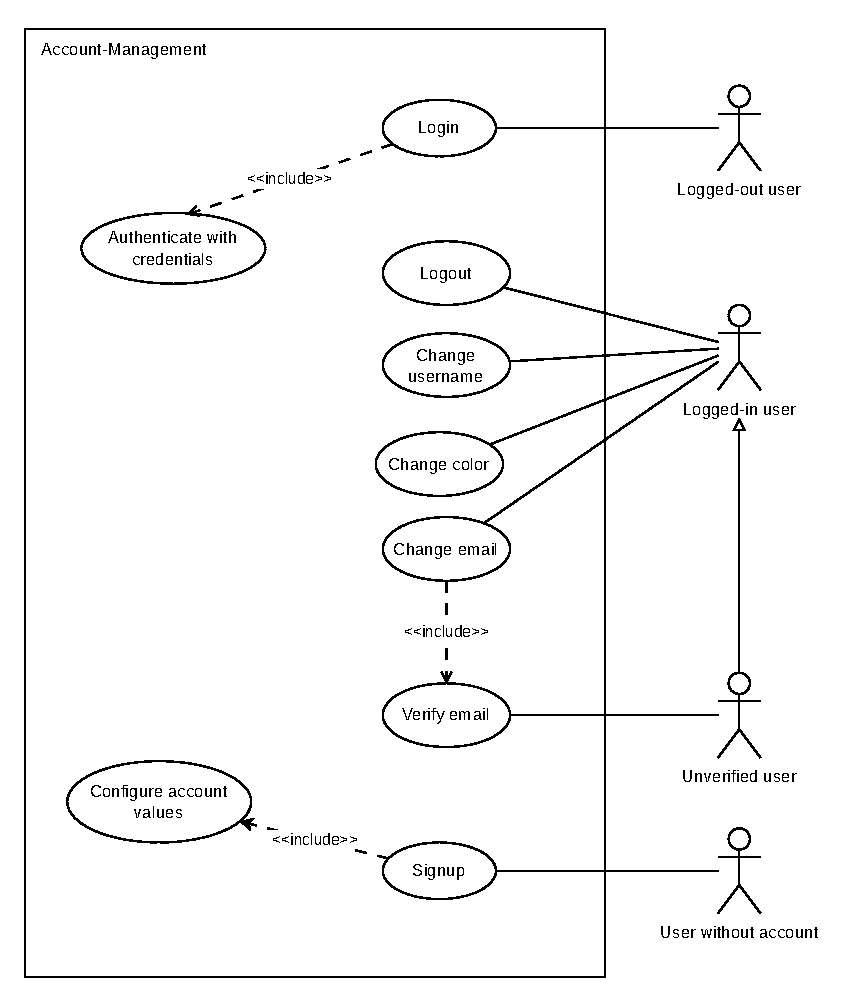
\includegraphics{uc-account-management}
    \caption{Use-cases for the account-management.}
    \label{fig:account-management}
\end{figure}

Figure~\ref{fig:account-management} shows the usecases related to authentication and management of the account.
We differentiate between
\begin{itemize}
    \item \textit{Logged-out users}: Users who are currently not logged in, but have access to crdentials to an account.
    \item \textit{Deactivated user}: Users who deactivated their own account.
    \item \textit{Logged-in user}: Users who are currently logged in and can perform actions.
    \item \textit{User without account}: Users who have never interacted with the system and can create a new account.
    \item \textit{Unverified user}: Users who are logged into an account that doesn't have their email verified.
\end{itemize}

\subsubsection{Admin panel}
\begin{figure}
    \centering
    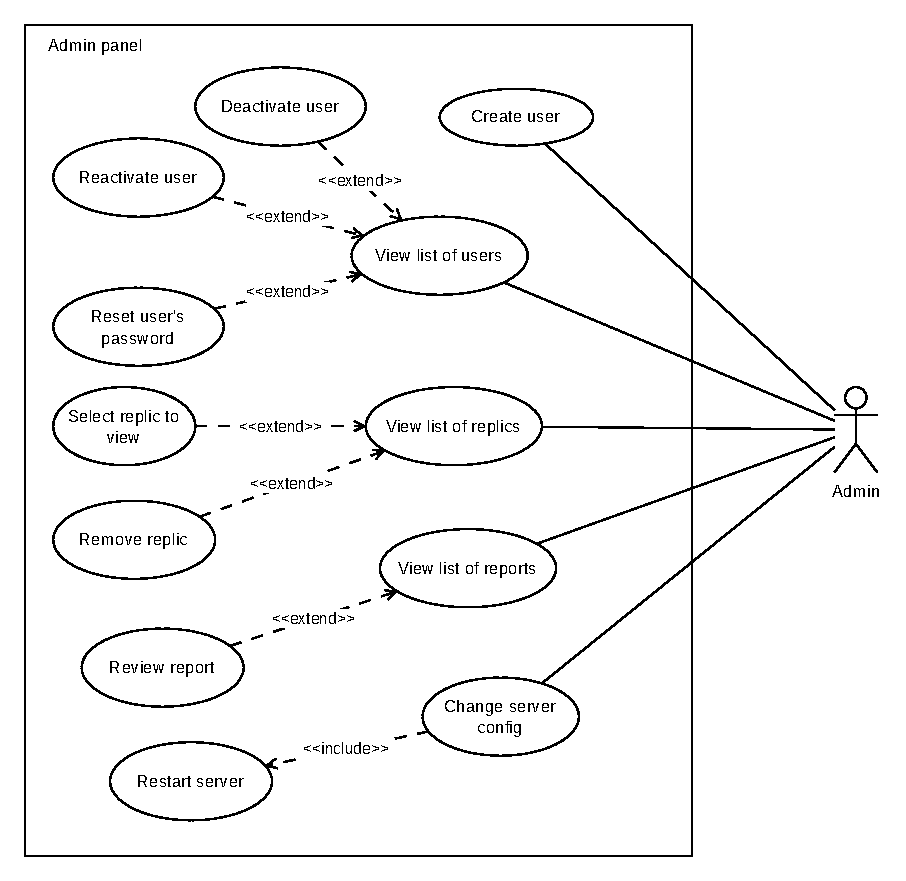
\includegraphics{uc-admin-panel}
    \caption{Use-cases for the admin-panel.}
    \label{fig:admin-panel}
\end{figure}

Figure~\ref{fig:admin-panel} shows the usecases related to the admin panel.
The only users that can interact with this subsystem are admin users.
Admin users have access to a list of users, replics and reports.
For each the have access to specific context actions to manipulate single items.

\subsubsection{Replic creation}
\begin{figure}
    \centering
    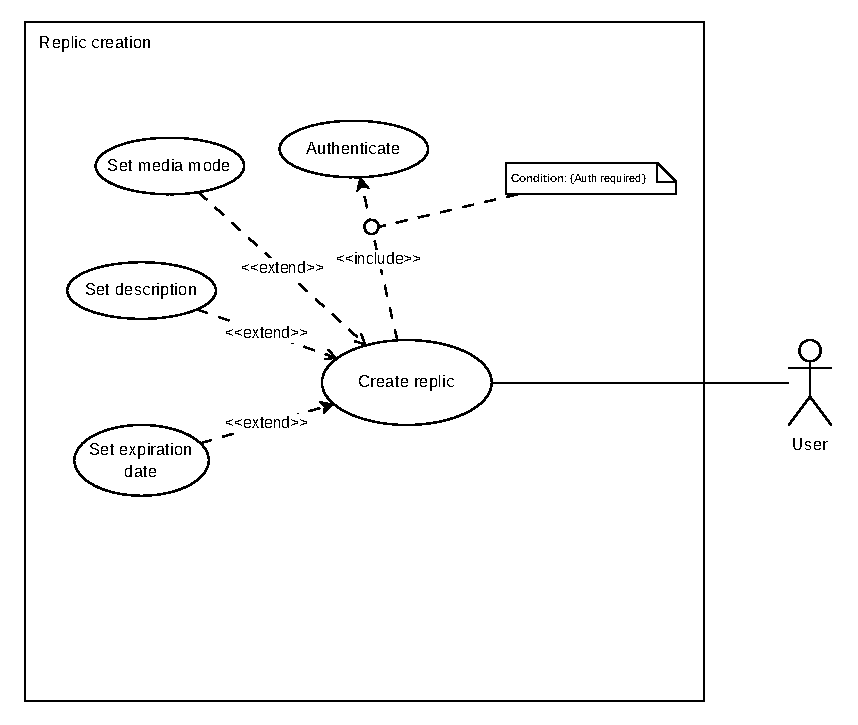
\includegraphics{uc-replic-creation}
    \caption{Use-cases for the replic-creation.}
    \label{fig:replic-creation}
\end{figure}

Figure~\ref{fig:replic-creation} shows the usecases for the subsystem that manages creating a single replic.
The base usecase of \("\)Create replic\("\) has many includes, that correspond to configurations of the replic that will be created.
\("\)Authenticate\("\) is only necessary if creating a replica requires authentication, a server-wide setting.

\subsubsection{Replic management}
\begin{figure}
    \centering
    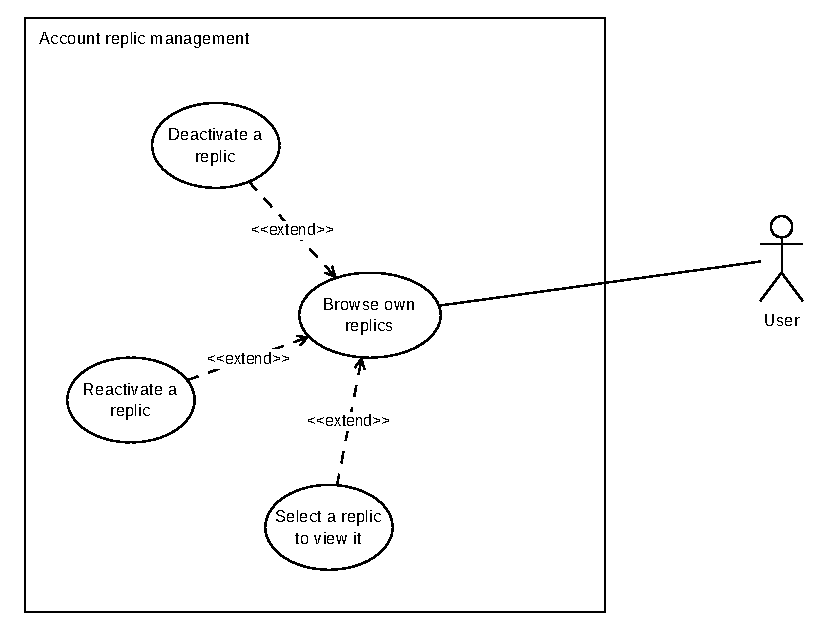
\includegraphics{uc-replic-management}
    \caption{Use-cases for the replic-management.}
    \label{fig:replic-management}
\end{figure}

Figure~\ref{fig:replic-management} shows the usecases for managing the replics of an account.
The main usecase \("\)Browse own replics\("\) has three context actions that allow to deactivate a replic, to reactivate a deactivated replic and to select and view a replic.

\subsubsection{Replic viewing}
\begin{figure}
    \centering
    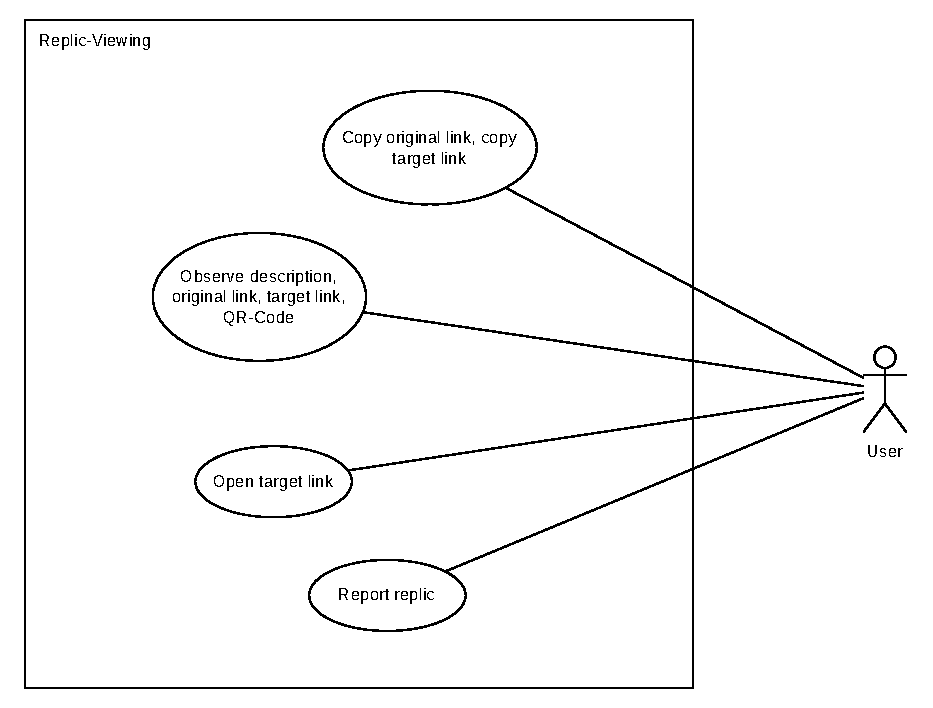
\includegraphics{uc-replic-viewing}
    \caption{Use-cases for the replic-viewing.}
    \label{fig:replic-viewing}
\end{figure}

Figure~\ref{fig:replic-viewing} shows the usecases for when a replic is being viewn.
The context actions are related to accessing the archived media, sharing and repeorting it.

\subsubsection{Miscellaneous}
\begin{figure}
    \centering
    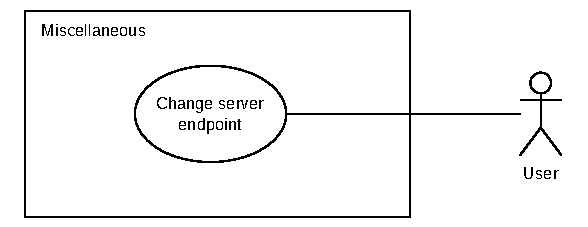
\includegraphics{uc-miscellaneous}
    \caption{Miscellaneous use-cases.}
    \label{fig:miscellaneous}
\end{figure}

Figure~\ref{fig:miscellaneous} shows general usecases that are not part of a specific subsystem.


    \section{Product features}\label{sec:product-features}
    \subsection{List of product features}\label{subsec:list-of-product-features}

\subsubsection{Login}\label{subsubsec:login}
\textbf{Use-case:} Login \newline
\textbf{Requirements:}~\ref{ac:accounts:3}~\ref{ac:accounts:4} \newline
\textbf{Target:} User is logged in and a session is created. \newline
\textbf{Condition:} The login-view is visible. \newline
\textbf{Postcondidion success:} The user is logged in. \newline
\textbf{Postcondition failure:} The user is not logged in. \newline
\textbf{Actors:} A user that is not logged into an account. \newline
\textbf{Event:} User clicks the login-button. \newline
\textbf{Description}: If the credentials of the user can be validated by the system, a session is created and the user redirected.
If the credentials are invalid, an error is shown.

\subsubsection{Logout}\label{subsubsec:logout}
\textbf{Use-case:} Logout \newline
\textbf{Requirements:}~\ref{ac:accounts:4} \newline
\textbf{Target:} User is logged out and the session gets removed. \newline
\textbf{Condition:} The account-view is visible. \newline
\textbf{Postcondidion success:} The user is logged out. \newline
\textbf{Postcondition failure:} The user is not logged out. \newline
\textbf{Actors:} A user that is logged in an account. \newline
\textbf{Event:} User clicks logout-button. \newline
\textbf{Description}: The session of the user is removed and the user redirected.

\subsubsection{Sign-up}\label{subsubsec:signup}
\textbf{Use-case:} Signup \newline
\textbf{Requirements:}~\ref{ac:accounts:4} \newline
\textbf{Target:} A new account will be created. \newline
\textbf{Condition:} The signup-view is visible. \newline
\textbf{Postcondidion success:} A new account is created. \newline
\textbf{Postcondition failure:} No new account is created. \newline
\textbf{Actors:} A user that is not logged in an account. \newline
\textbf{Event:} The user clicks the signup button. \newline
\textbf{Description}: If the system fails to validate the username and password, an error is shown.
Otherwise, the account is created, the user logged in and redirected.

\subsubsection{Change username}\label{subsubsec:change-username}
\textbf{Use-case:} Change username \newline
\textbf{Requirements:}~\ref{ac:accounts:2} \newline
\textbf{Target:} The username will be changed. \newline
\textbf{Condition:} The account-view is visible. \newline
\textbf{Postcondidion success:} The username was changed. \newline
\textbf{Postcondition failure:} The username was not changed. \newline
\textbf{Actors:} A user that is logged in an \textit{active} account. \newline
\textbf{Event:} The user clicks the confirm button. \newline
\textbf{Description}: If the system fails to validate the username, an error is shown.
Otherwise, the username is changed and shown to the user.

\subsubsection{Change email}\label{subsubsec:change-email}
\textbf{Use-case:} Change email \newline
\textbf{Requirements:}~\ref{ac:accounts:2} \newline
\textbf{Target:} A verification-email is sent. \newline
\textbf{Condition:} The account-view is visible. \newline
\textbf{Postcondidion success:} A verification-email is sent to the new email. \newline
\textbf{Postcondition failure:} No verification-email was sent. \newline
\textbf{Actors:} A user that is logged in an \textit{active} account. \newline
\textbf{Event:} The user clicks the save changes button. \newline
\textbf{Description}: After the user saves the changes, the system sends an email-verification email to the new email-address submitted by the user.
The user then has the oppurtinity opportunity to verify the new email-address by using the token in the email.

\subsubsection{Change color}\label{subsubsec:change-color}
\textbf{Use-case:} Change color \newline
\textbf{Requirements:}~\ref{ac:accounts:2} \newline
\textbf{Target:} The color will be changed. \newline
\textbf{Condition:} The profile-view is visible. \newline
\textbf{Postcondidion success:} The color was changed. \newline
\textbf{Postcondition failure:} The color was not changed. \newline
\textbf{Actors:} A user that is logged in an \textit{active} account. \newline
\textbf{Event:} The user clicks the confirm button. \newline
\textbf{Description}: The color is changed and shown to the user.

\subsubsection{Creating a replic}\label{subsubsec:create-replic}
\textbf{Use-case:} Create replic \newline
\textbf{Requirements:}~\ref{ac:replics:1}~\ref{ac:replics:2}~\ref{ac:replics:3}~\ref{ac:replics:4} \newline
\textbf{Target:} A new replic will be created. \newline
\textbf{Condition:} The user has the target tab opened in the browser.
The create-replic-view is visible. \newline
\textbf{Postcondidion success:} A new replic is created. \newline
\textbf{Postcondition failure:} No new replic is created. \newline
\textbf{Actors:} A user.
If required by the server, the user is logged in an \textit{active} account. \newline
\textbf{Event:} The user configures the replic settings and clicks the confirmation button. \newline
\textbf{Description}: The system gathers the content and creates a replic.
An informative message with a link to the replic is shown to the user.

\subsubsection{Deactivating a replic}\label{subsubsec:deactivate-replic}
\textbf{Use-case:} Deactivate replic \newline
\textbf{Requirements:}~\ref{ac:replics:5} \newline
\textbf{Target:} The replic will be \textit{inactive}. \newline
\textbf{Condition:} The account of the user owns the replic.
The replic must be~\textit{active}.
The own-replics-view is visible. \newline
\textbf{Postcondidion success:} The replic is \textit{inactive}. \newline
\textbf{Postcondition failure:} The replic is not \textit{inactive}. \newline
\textbf{Actors:} A user that is logged into an \textit{active} account. \newline
\textbf{Event:} The user clicks the deactivation button on the replic. \newline
\textbf{Description}: The sets the replic to \textit{inactive}.

\subsubsection{Reactivating a replic}\label{subsubsec:reactivate-replic}
\textbf{Use-case:} Reactivate replic \newline
\textbf{Requirements:}~\ref{ac:replics:5} \newline
\textbf{Target:} The replic will be~\textit{active}. \newline
\textbf{Condition:} The account of the user owns the replic.
The replic must be~\textit{inactive}.
The own-replics-view is visible. \newline
\textbf{Postcondidion success:} The replic is~\textit{active}. \newline
\textbf{Postcondition failure:} The replic is not~\textit{active}. \newline
\textbf{Actors:} A user that is logged into an \textit{active} account. \newline
\textbf{Event:} The user clicks the reactivation button on the replic. \newline
\textbf{Description}: The system sets the replic to \textit{active}.

\subsubsection{Selecting a replic}\label{subsubsec:select-replic}
\textbf{Use-case:} Select a replic to view it \newline
\textbf{Requirements:}~\ref{ac:replics:7} \newline
\textbf{Target:} The view-replic screen will be opened. \newline
\textbf{Condition:} The own-replics-view is visible. \newline
\textbf{Postcondidion success:} The replic is shown. \newline
\textbf{Postcondition failure:} The replic is not shown. \newline
\textbf{Actors:} A user. \newline
\textbf{Event:} The user selects a replic, e.g.\ by clicking on it in an overview, entering the link in the browser or scanning the QR-code. \newline
\textbf{Description}: If the access-level is \textit{none}, the user is redirected to the replic-view.
If the access-level is \textit{password}, the user is redirected to the screen where the password for the replic can be entered.
Upon entering the correct password, the user is redirected to the replic-screen, otherwise shown an error.
If the access-level is \textit{authenticated}, the user is redirected to the login-view if it is unauthenticated, otherwise the user is directly redirected to the replic-view.

\subsubsection{Report replic}\label{subsubsec:report-replic}
\textbf{Use-case:} Report replic \newline
\textbf{Requirements:}~\ref{ac:reports:1} \newline
\textbf{Target:} A report will be created. \newline
\textbf{Condition:} The replic-view is visible.
If required by the server, the user is logged into an \textit{active} account. \newline
\textbf{Postcondidion success:} A report is created. \newline
\textbf{Postcondition failure:} No report is created. \newline
\textbf{Actors:} A user. \newline
\textbf{Event:} The user submits the report. \newline
\textbf{Description}: The system creates a report.

\subsubsection{Copy replic links}\label{subsubsec:copy-replic-links}
\textbf{Use-case:} Copy original link, copy target link \newline
\textbf{Requirements:}~\ref{ac:replics:7} \newline
\textbf{Target:} The selected link will be copied. \newline
\textbf{Condition:} The replic-view is visible. \newline
\textbf{Postcondidion success:} The link has been copied. \newline
\textbf{Postcondition failure:} The link has not been copied. \newline
\textbf{Actors:} A user. \newline
\textbf{Event:} The user clicks the copy button on the respective link. \newline
\textbf{Description}: The respective link is copied into the user's clipboard.

\subsubsection{Viewing a replic}\label{subsubsec:view-replic}
\textbf{Use-case:} Observe description, original link, target link, QR-code \newline
\textbf{Requirements:}~\ref{ac:replics:7} \newline
\textbf{Target:} The replic data is shown. \newline
\textbf{Condition:} The user can fulfill the requirements by the access-level. \newline
\textbf{Postcondidion success:} The data is shown. \newline
\textbf{Postcondition failure:} The data is not shown. \newline
\textbf{Actors:} A user. \newline
\textbf{Event:} The user is directed to the replic-view screen. \newline
\textbf{Description}: The user can view the data related to the replic, e.g.\ the links, access-level etc..

\subsubsection{Open target link}\label{subsubsec:open-target-link}
\textbf{Use-case:} Open target link \newline
\textbf{Requirements:}~\ref{ac:replics:7}\newline
\textbf{Target:} The replic's captured media document is opened in another browser tab. \newline
\textbf{Condition:} The replic-view is visible. \newline
\textbf{Postcondidion success:} The new tab is opened. \newline
\textbf{Postcondition failure:} The new tab is not opened. \newline
\textbf{Actors:} A user that can view the replic. \newline
\textbf{Event:} The clicks on the button to open the replic's media. \newline
\textbf{Description}: The user is directed to a new tab that points to the URL that contains the saved media of the replic.

\subsubsection{Change server endpoint}\label{subsubsec:change-server-endpoint}
\textbf{Use-case:} Change server endpoint \newline
\textbf{Requirements:} \newline
\textbf{Target:} The clients endpoint is changed. \newline
\textbf{Condition:} The change-endpoint-view is visible. \newline
\textbf{Postcondidion success:} The endpoint is changed. \newline
\textbf{Postcondition failure:} The endpoint is not changed. \newline
\textbf{Actors:} A user. \newline
\textbf{Event:} The user clicks on the button to change the clients endpoint. \newline
\textbf{Description}: After the user clicks the button to confirm the change.
The provided endpoint is validated.
If the endpoint is valid, the client state is reset, i.e.\ saved data, tokens etc.\ are removed from the local cache.
This also means the user is logged out.

\subsubsection{Create account (admin)}\label{subsubsec:create-user}
\textbf{Use-case:} Create account \newline
\textbf{Requirements:}~\ref{ac:admins:9} \newline
\textbf{Target:} A new account is created. \newline
\textbf{Condition:} The admin-panel is visible. \newline
\textbf{Postcondidion success:} A user is created. \newline
\textbf{Postcondition failure:} No user is created. \newline
\textbf{Actors:} A user. \newline
\textbf{Event:} The user clicks on the create-user button. \newline
\textbf{Description}: After the user clicks the button to confirm the creation, a new account is created.

\subsubsection{Review report (Admin)}\label{subsubsec:review-report}
\textbf{Use-case:} Review report \newline
\textbf{Requirements:}~\ref{ac:admins:7} \newline
\textbf{Target:} The report will be set to reviewed. \newline
\textbf{Condition:} The all-reports-view is visible.
The report is \textit{open}. \newline
\textbf{Postcondidion success:} The report is \textit{reviewed}. \newline
\textbf{Postcondition failure:} The report is not \textit{reviewed}. \newline
\textbf{Actors:} A user that is logged in an admin-account. \newline
\textbf{Event:} The user clicks the review-replic button. \newline
\textbf{Description}: The system sets the report to \textit{reviewed}.

\subsubsection{Restart server (Admin)}\label{subsubsec:restart-server}
\textbf{Use-case:} Restart server \newline
\textbf{Requirements:}~\ref{ac:admins:8} \newline
\textbf{Target:} The server will queue up a restart. \newline
\textbf{Condition:} The server is running. \newline
\textbf{Postcondidion success:} The server is restarting. \newline
\textbf{Postcondition failure:} The server is still running. \newline
\textbf{Actors:} A user that is logged in an admin-account. \newline
\textbf{Event:} The user clicks the restart-server button. \newline
\textbf{Description}: The system restarts the server.

\subsubsection{Reactivating an account (Admin)}\label{subsubsec:reactivate-acc-admin}
\textbf{Use-case:} Reactivate account \newline
\textbf{Requirements:}~\ref{ac:admins:6} \newline
\textbf{Target:} An account will be \textit{active}. \newline
\textbf{Condition:} The target account is currently \textit{force-inactive}.
The all-accounts-view is visble. \newline
\textbf{Postcondidion success:} The account is \textit{active}. \newline
\textbf{Postcondition failure:} The account is not \textit{active}. \newline
\textbf{Actors:} A user that is logged in an admin-account. \newline
\textbf{Event:} The user clicks the reactivate button. \newline
\textbf{Description}: The system sets the target account to \textit{active}

\subsubsection{Deactivating an account (Admin)}\label{subsubsec:deactivate-acc-admin}
\textbf{Use-case:} Deactivate account \newline
\textbf{Requirements:}~\ref{ac:admins:6} \newline
\textbf{Target:} The target account will be \textit{force-inactive}. \newline
\textbf{Condition:} The account is currently \textit{active}.
The all-accounts-view is visible. \newline
\textbf{Postcondidion success:} The account is \textit{force-inactive}. \newline
\textbf{Postcondition failure:} The account is still \textit{force-inactive}. \newline
\textbf{Actors:} A user that is logged into an admin-account. \newline
\textbf{Event:} The user clicks the deactivate button. \newline
\textbf{Description}: The system sets the target account to \textit{force-inactive}

\subsubsection{Reset password (Admin)}\label{subsubsec:reset-pass}
\textbf{Use-case:} Reset account's password \newline
\textbf{Requirements:}~\ref{ac:admins:4} \newline
\textbf{Target:} The password of the target account will be reset. \newline
\textbf{Condition:} The all-accounts-view is visible. \newline
\textbf{Postcondidion success:} The password is reset. \newline
\textbf{Postcondition failure:} The password has not been reset. \newline
\textbf{Actors:} A user that is logged in an admin-account. \newline
\textbf{Event:} The user clicks the reset-password button. \newline
\textbf{Description}: If the system fails to validate the password, an error message is shown.
Otherwise, the user's password is changed.

\subsubsection{Remove replic (Admin)}\label{subsubsec:remove-replic}
\textbf{Use-case:} Remove replic \newline
\textbf{Requirements:}~\ref{ac:admins:5} \newline
\textbf{Target:} The replic will be \textit{force-inactive}. \newline
\textbf{Condition:} The all-replics-view is visible.
The replic must be \textit{active} \newline
\textbf{Postcondidion success:} The replic is \textit{force-inactive}. \newline
\textbf{Postcondition failure:} The replic is not \textit{force-inactive}. \newline
\textbf{Actors:} A user that is logged in an admin-account. \newline
\textbf{Event:} The user clicks the remove-replic button. \newline
\textbf{Description}: The system sets the replic to \textit{removed}.

\subsection{Activity diagrams}\label{subsec:activity-diagrams}
In the following, the more complex product features will be described in activity-diagrams.

\subsubsection{Login}
\begin{figure}
    \centering
    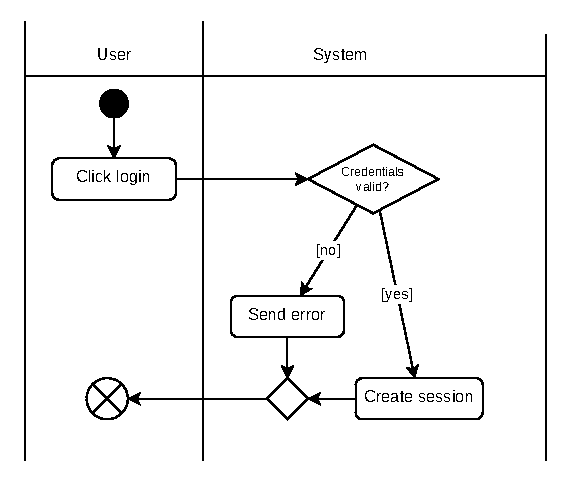
\includegraphics{ad-login}
    \caption{Activity diagram for the login flow.}
    \label{fig:ad:login}
\end{figure}

Figure~\ref{fig:ad:login} shows the steps that are required for the login process to finish.
The process ends either when the user has been logged in, and a session was created, or when the user failed to login.

\subsubsection{Signup}
\begin{figure}
    \centering
    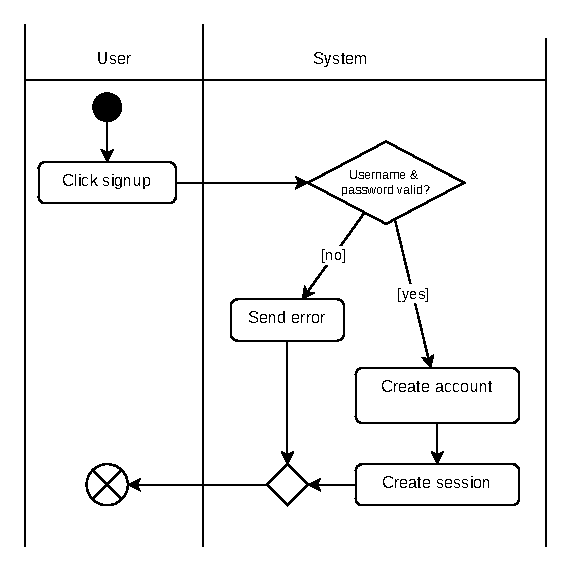
\includegraphics{ad-signup}
    \caption{Activity diagram for the signup flow.}
    \label{fig:ad:signup}
\end{figure}

Figure~\ref{fig:ad:signup} shows the steps that are required for the signup process to finish.
The process ends either when an account and session has been created, or when the user failed to signup.

\subsubsection{Select replic}
\begin{figure}
    \centering
    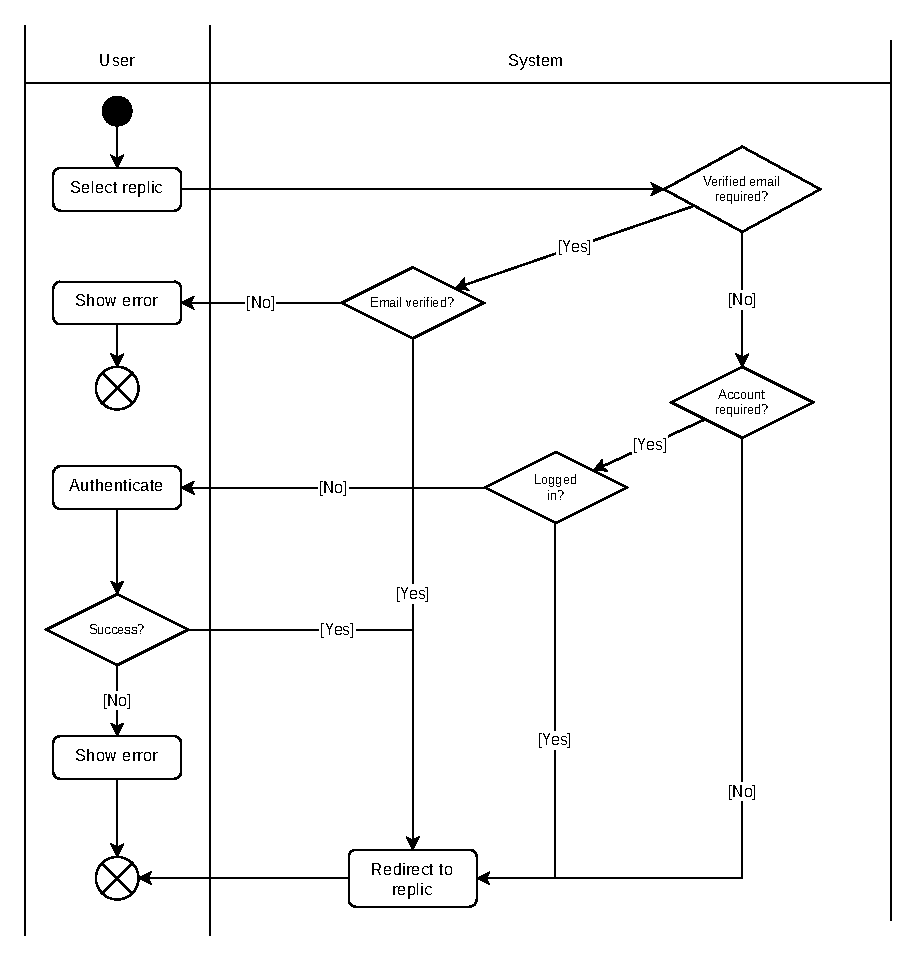
\includegraphics{ad-select-replic}
    \caption{Activity diagram for the select-replic flow.}
    \label{fig:ad:select-replic}
\end{figure}

Figure~\ref{fig:ad:select-replic} shows the steps to be done when the user selects a replic.
The outcome depends mostly on the access-level.
The flow finishes either when the user was redirected to the replic, or when the user could not be redirected.


    \section{Nonfunctional criteria}\label{sec:nonfunctional-criteria}
    \subsection{Security}\label{subsec:security}
\begin{enumerate}[label=\textit{NF\arabic*}]
    \item \label{nf:1} Passwords are not stored in cleartext in the database.
    \item \label{nf:2} Communication to the server is only possible via HTTPS\@.
\end{enumerate}

\subsection{User interaction}\label{subsec:user-interaction}
\begin{enumerate}[label=\textit{NF\arabic*}, resume]
    \item \label{nf:3} Invalid user input is clearly communicated to the user, and instructions given how to resolve the problem.
    \item \label{nf:4} The client's interfaces are accessible.
\end{enumerate}


    \section{User interface}\label{sec:user-interface}
    This chapter contains mockups of the user interface of the components the user interacts with.
While the mockups are aimed to be as precise as possible, they will not resemble the final layout and design.

\subsection{Browser extension}\label{subsec:browser-extension}
The user-interface for the browser extension will run inside the browser of the user.
The size of the window occupied by the extension will be around \SI{400}{px}--\SI{600}{px}. \newline
These constraints require the interface of the extension to be extremely simplistic and only display the minimal required amount of data and actions to not overwhelm the user.

\subsubsection{Login view}
The login screen (\ref{fig:ex-login-view}) allows the user to login (\ref{subsubsec:login}), or to navigate to the signup view (\ref{fig:ex-signup-view}) if an account should be created.
\begin{figure}
    \centering
    \fbox{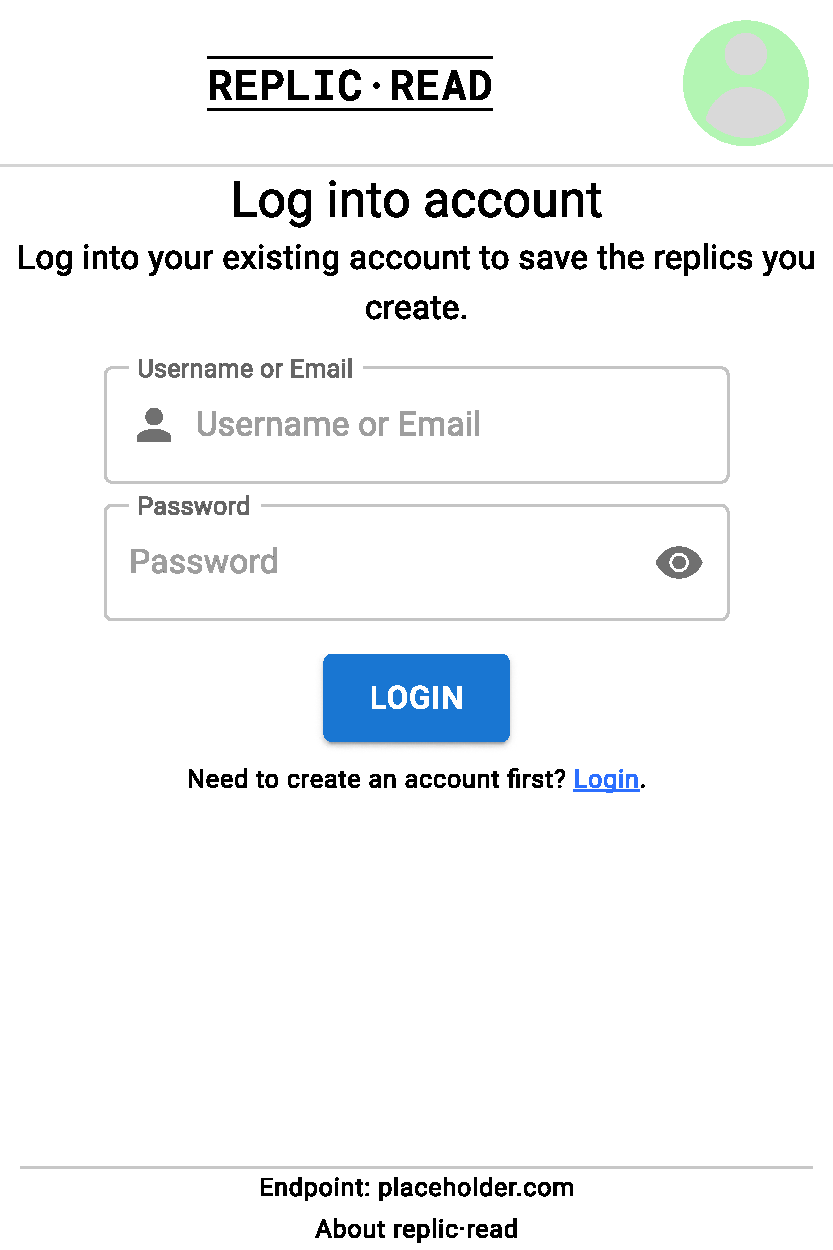
\includegraphics[height=15cm]{ex-login}}

    \caption{Login view}
    \label{fig:ex-login-view}
\end{figure}

\subsubsection{Signup view}
The signup screen (\ref{fig:ex-signup-view}) allows the user to signup (\ref{subsubsec:signup}), or to navigate to the login screen (\ref{fig:ex-login-view}).
\begin{figure}
    \centering
    \fbox{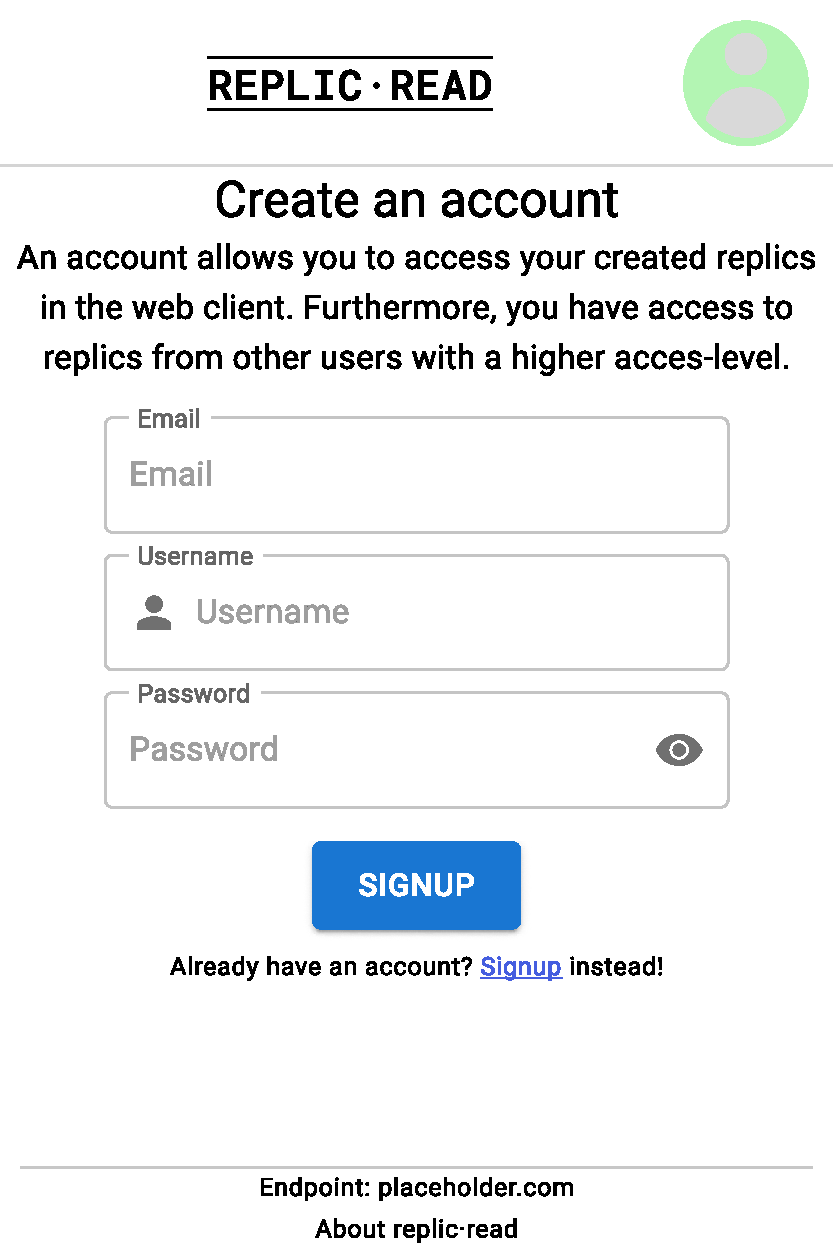
\includegraphics[height=15cm]{ex-signup}}

    \caption{Signup view}
    \label{fig:ex-signup-view}
\end{figure}

\subsubsection{Create replic view}
The create replic view allows a user to create a replic (\ref{subsubsec:create-replic}).
The configuration-panel can be collapsed (\ref{fig:ex-create-replic-view-collapsed}) or expanded (\ref{fig:ex-create-replic-view-expanded}). \newline
After the replic has been created, the user is redirected to (\ref{fig:ex-created-replic-view}).
\begin{figure}
    \centering
    \fbox{
\includegraphics[height=15cm]{ex-create-replic-collapsed}}

    \caption{Create replic view with the configuration menu collapsed}
    \label{fig:ex-create-replic-view-collapsed}
\end{figure}
\begin{figure}
    \centering
    \fbox{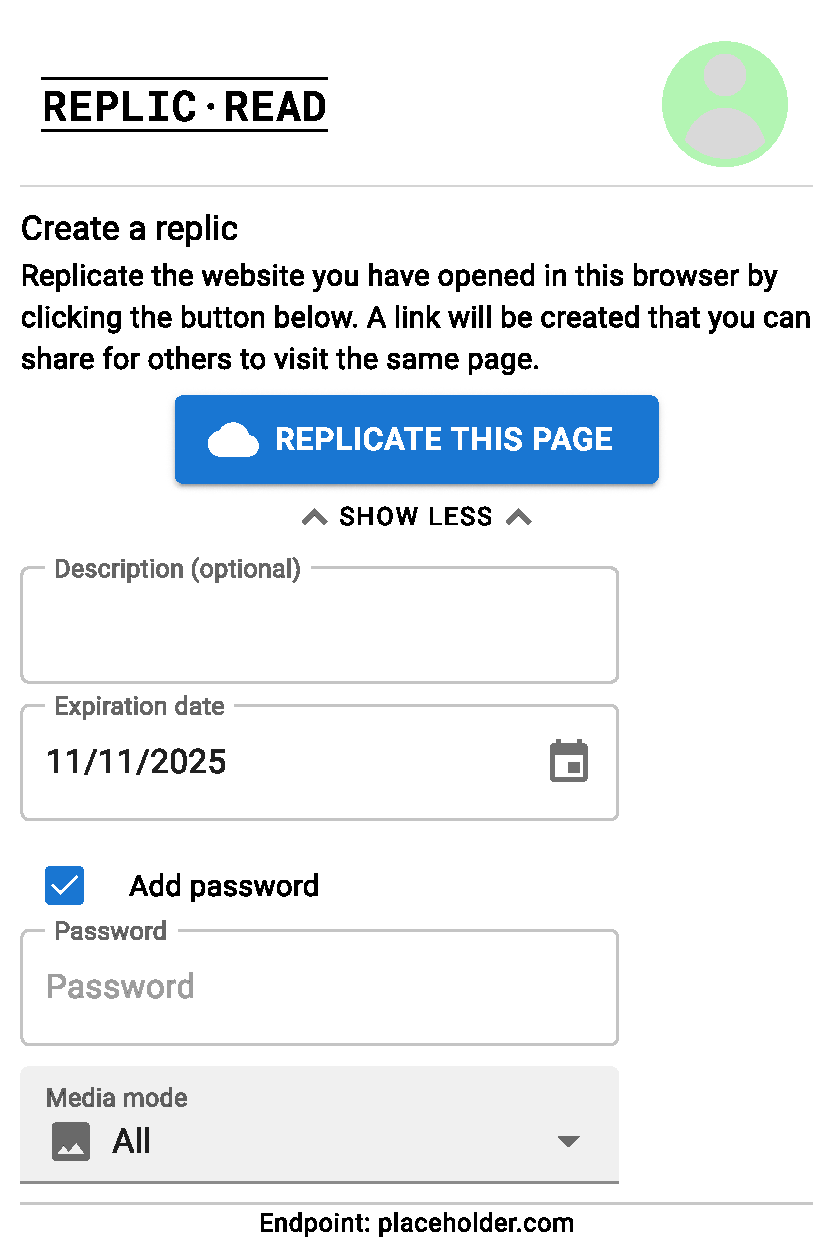
\includegraphics[height=15cm]{ex-create-replic-expanded}}

    \caption{Create replic view with the configuration menu expanded}
    \label{fig:ex-create-replic-view-expanded}
\end{figure}

\subsubsection{Replic created view}
The replic created view shows the user a quick summary of the created replic.
Additionally, the user can copy the target link of the replic that was created (\ref{subsubsec:create-replic}). \newline
A button to create another replic is shown, which will take the user back to the create replic view (\ref{fig:ex-create-replic-view-collapsed})
\begin{figure}
    \centering
    \fbox{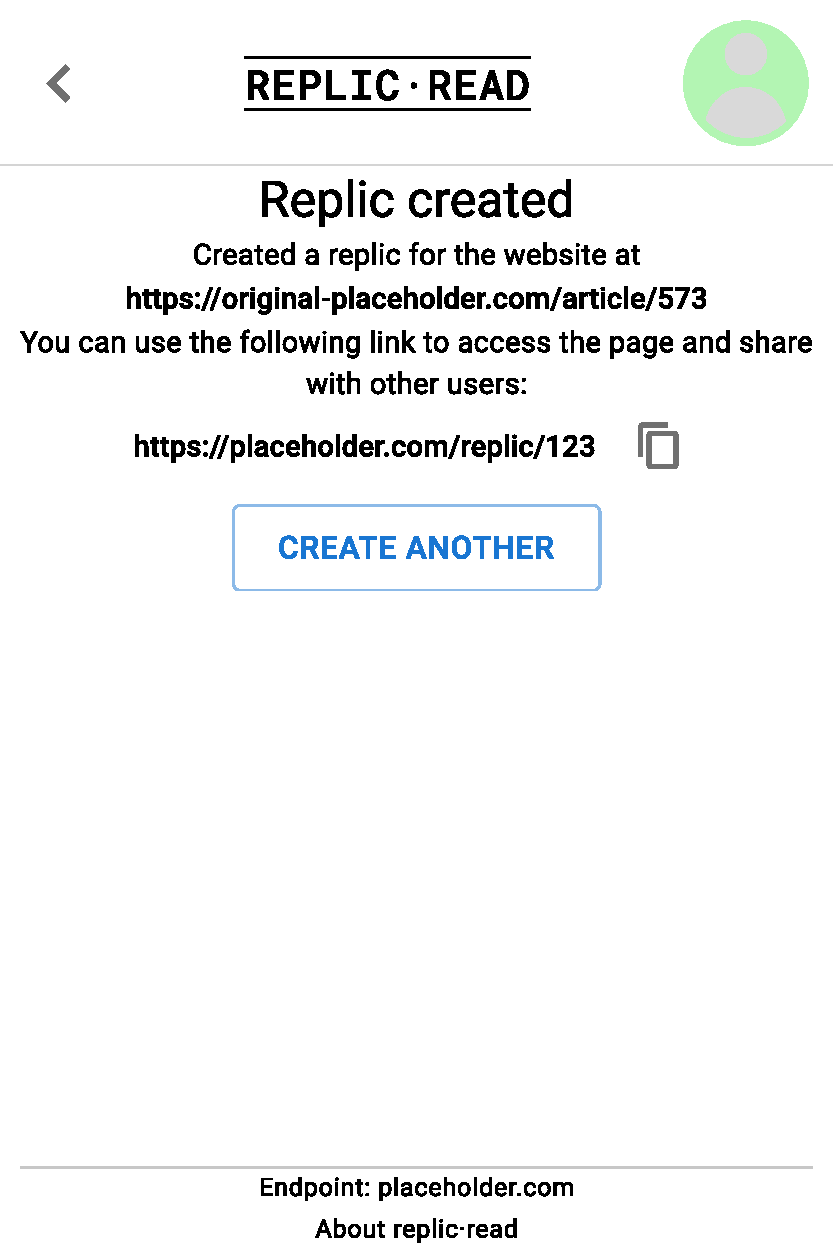
\includegraphics[height=15cm]{ex-replic-created}}

    \caption{Create replic view with the configuration menu expanded}
    \label{fig:ex-created-replic-view}
\end{figure}

\subsubsection{Change endpoint view}
The change endpoint view allows the user to set/change the endpoint the client connects to (\ref{subsubsec:change-server-endpoint}).
This view is navigated to by clicking the endpoint info in the footer. \newline
Depending on whether the user is logged in or -out, and whether an endpoint has already been set, one of~\ref{fig:ex-change-endpoint-view-none-logged-out},~\ref{fig:ex-change-endpoint-view-present-logged-out},~\ref{fig:ex-change-endpoint-view-present-logged-in} is shown.
\begin{figure}
    \centering
    \fbox{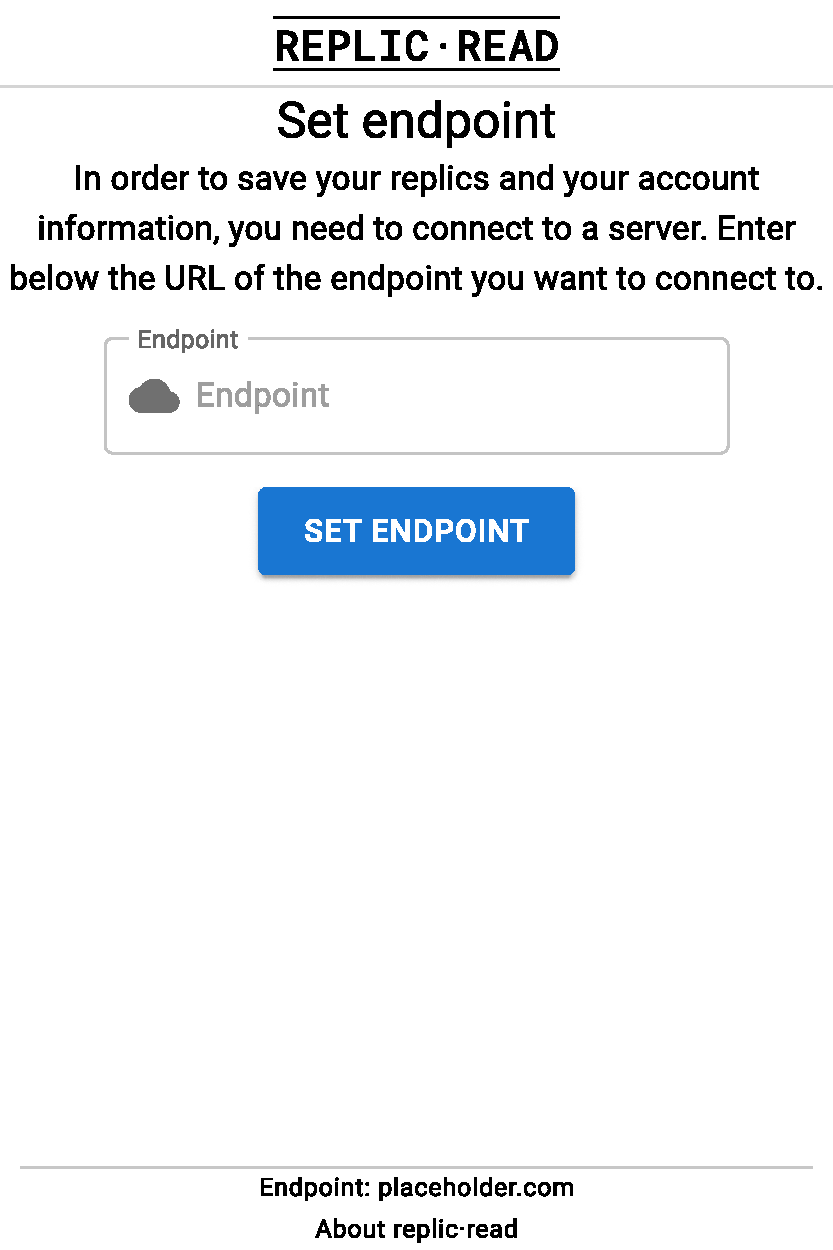
\includegraphics[height=15cm]{ex-change-endpoint-none-logged-out}}

    \caption{Change endpoint screen when the endpoint has to be initially set, and the user is logged out.}
    \label{fig:ex-change-endpoint-view-none-logged-out}
\end{figure}
\begin{figure}
    \centering
    \fbox{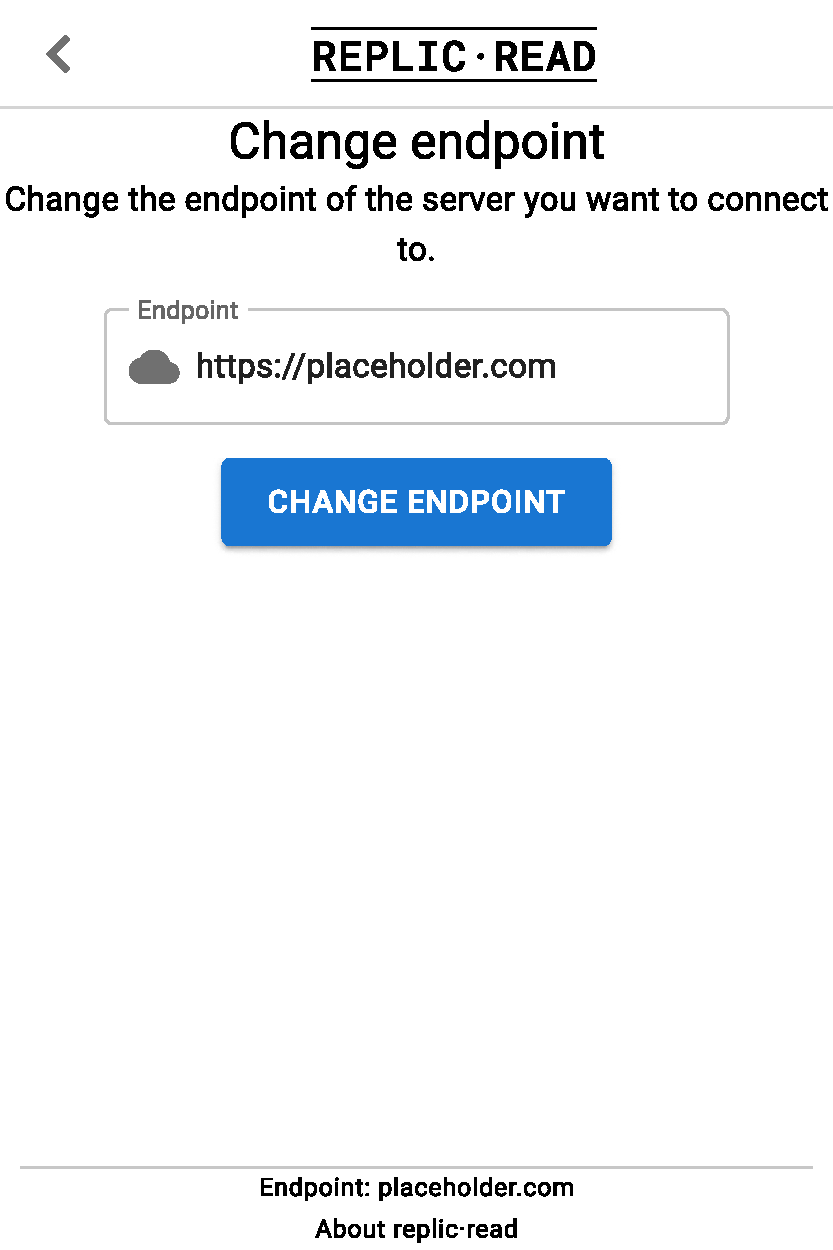
\includegraphics[height=15cm]{ex-change-endpoint-present-logged-out}}

    \caption{Change endpoint screen when the endpoint has already been set, and the user is logged out.}
    \label{fig:ex-change-endpoint-view-present-logged-out}
\end{figure}
\begin{figure}
    \centering
    \fbox{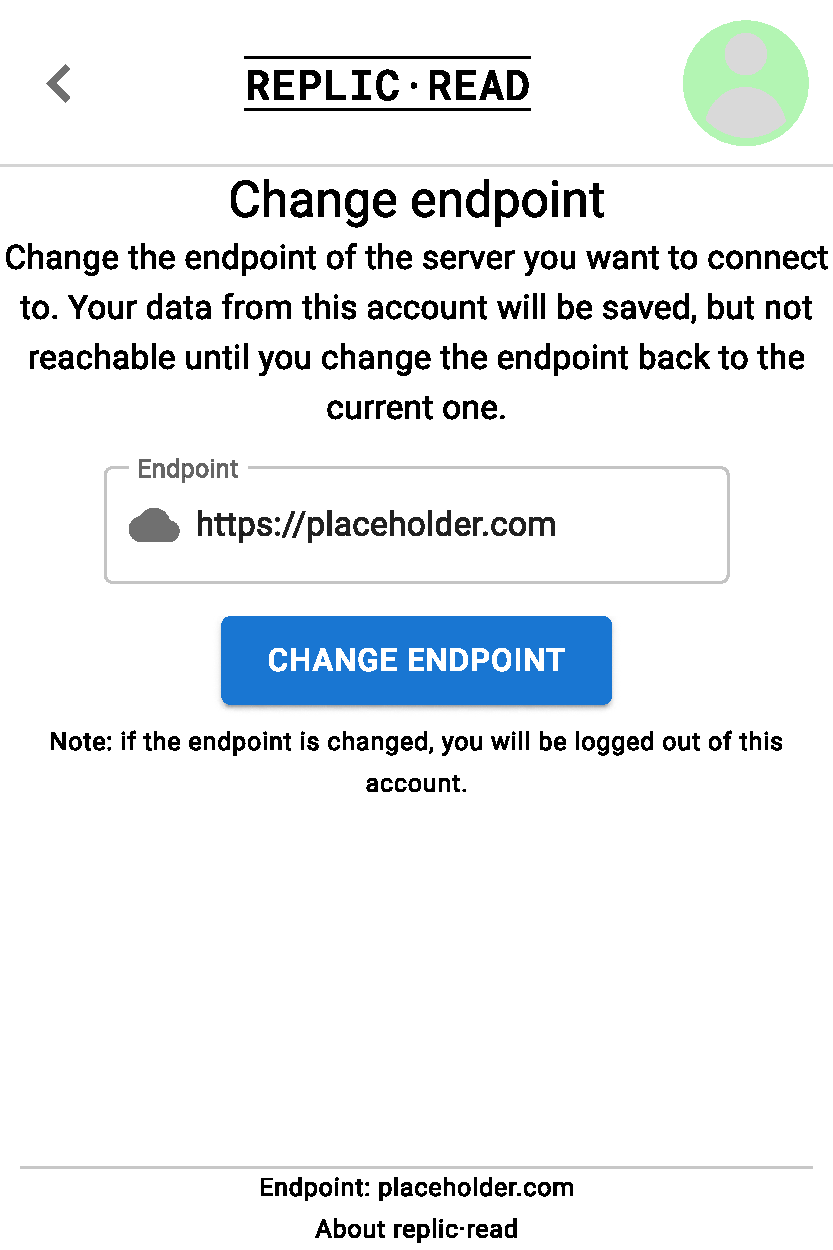
\includegraphics[height=15cm]{ex-change-endpoint-present-logged-in}}

    \caption{Change endpoint screen when the endpoint has already been set, and the user is logged in.}
    \label{fig:ex-change-endpoint-view-present-logged-in}
\end{figure}

\subsubsection{Account menu}
The account menu (\ref{fig:ex-account-menu-view}) gives context actions for the user related to the account, namely to logout (\ref{subsubsec:logout}).
Clicking on the account icon in the top right-hand corner navigates here.

\begin{figure}
    \centering
    \fbox{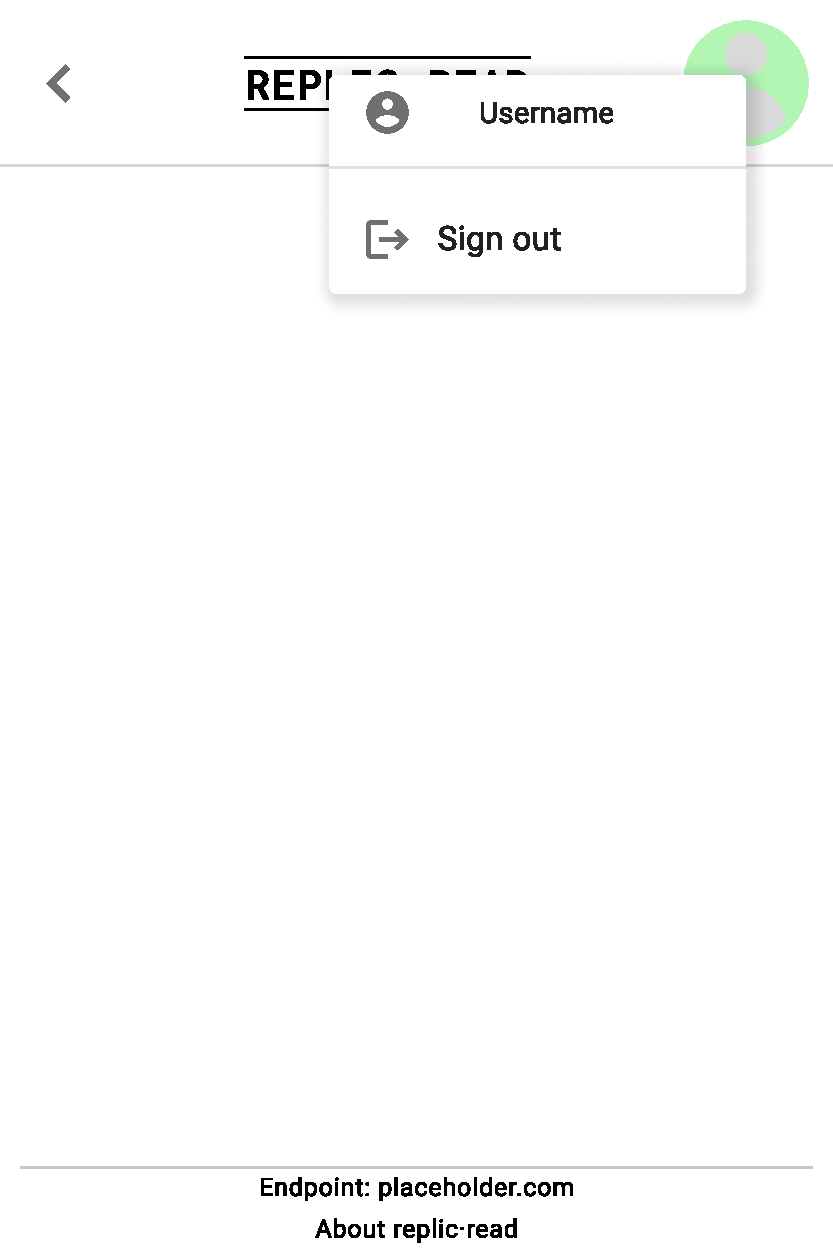
\includegraphics[height=15cm]{ex-account-menu}}

    \caption{Account menu.}
    \label{fig:ex-account-menu-view}
\end{figure}

\subsubsection{Unverified account view}
The account-not-verified view (\ref{fig:ex-account-not-verified-view}) shows an informative text to notify the user that the email has not yet been verified.
The user also has the option to request a new link.

\begin{figure}
    \centering
    \fbox{
\includegraphics[height=15cm]{ex-account-not-verified}}

    \caption{Account not yet verified.}
    \label{fig:ex-account-not-verified-view}
\end{figure}

\subsection{Web-Client}\label{subsec:web-client}
The user-interface for the web-client will run in any browser thatis supported.
Mobile-adaptive layouts are not supported.
The following graphics depict the screens on a default \SI{400}{px} by \SI{600}{px} desktop environment.
Due to size constraints, the mockups are presented in small display.
The full-size graphics can be found in the appendix.

\subsubsection{Login View}
The login screen (\ref{fig:web-login-view}) allows the user to login (\ref{subsubsec:login}), or to navigate to the signup view (\ref{fig:web-signup-view}) if an account should be created.
\begin{figure}
    \centering
    \fbox{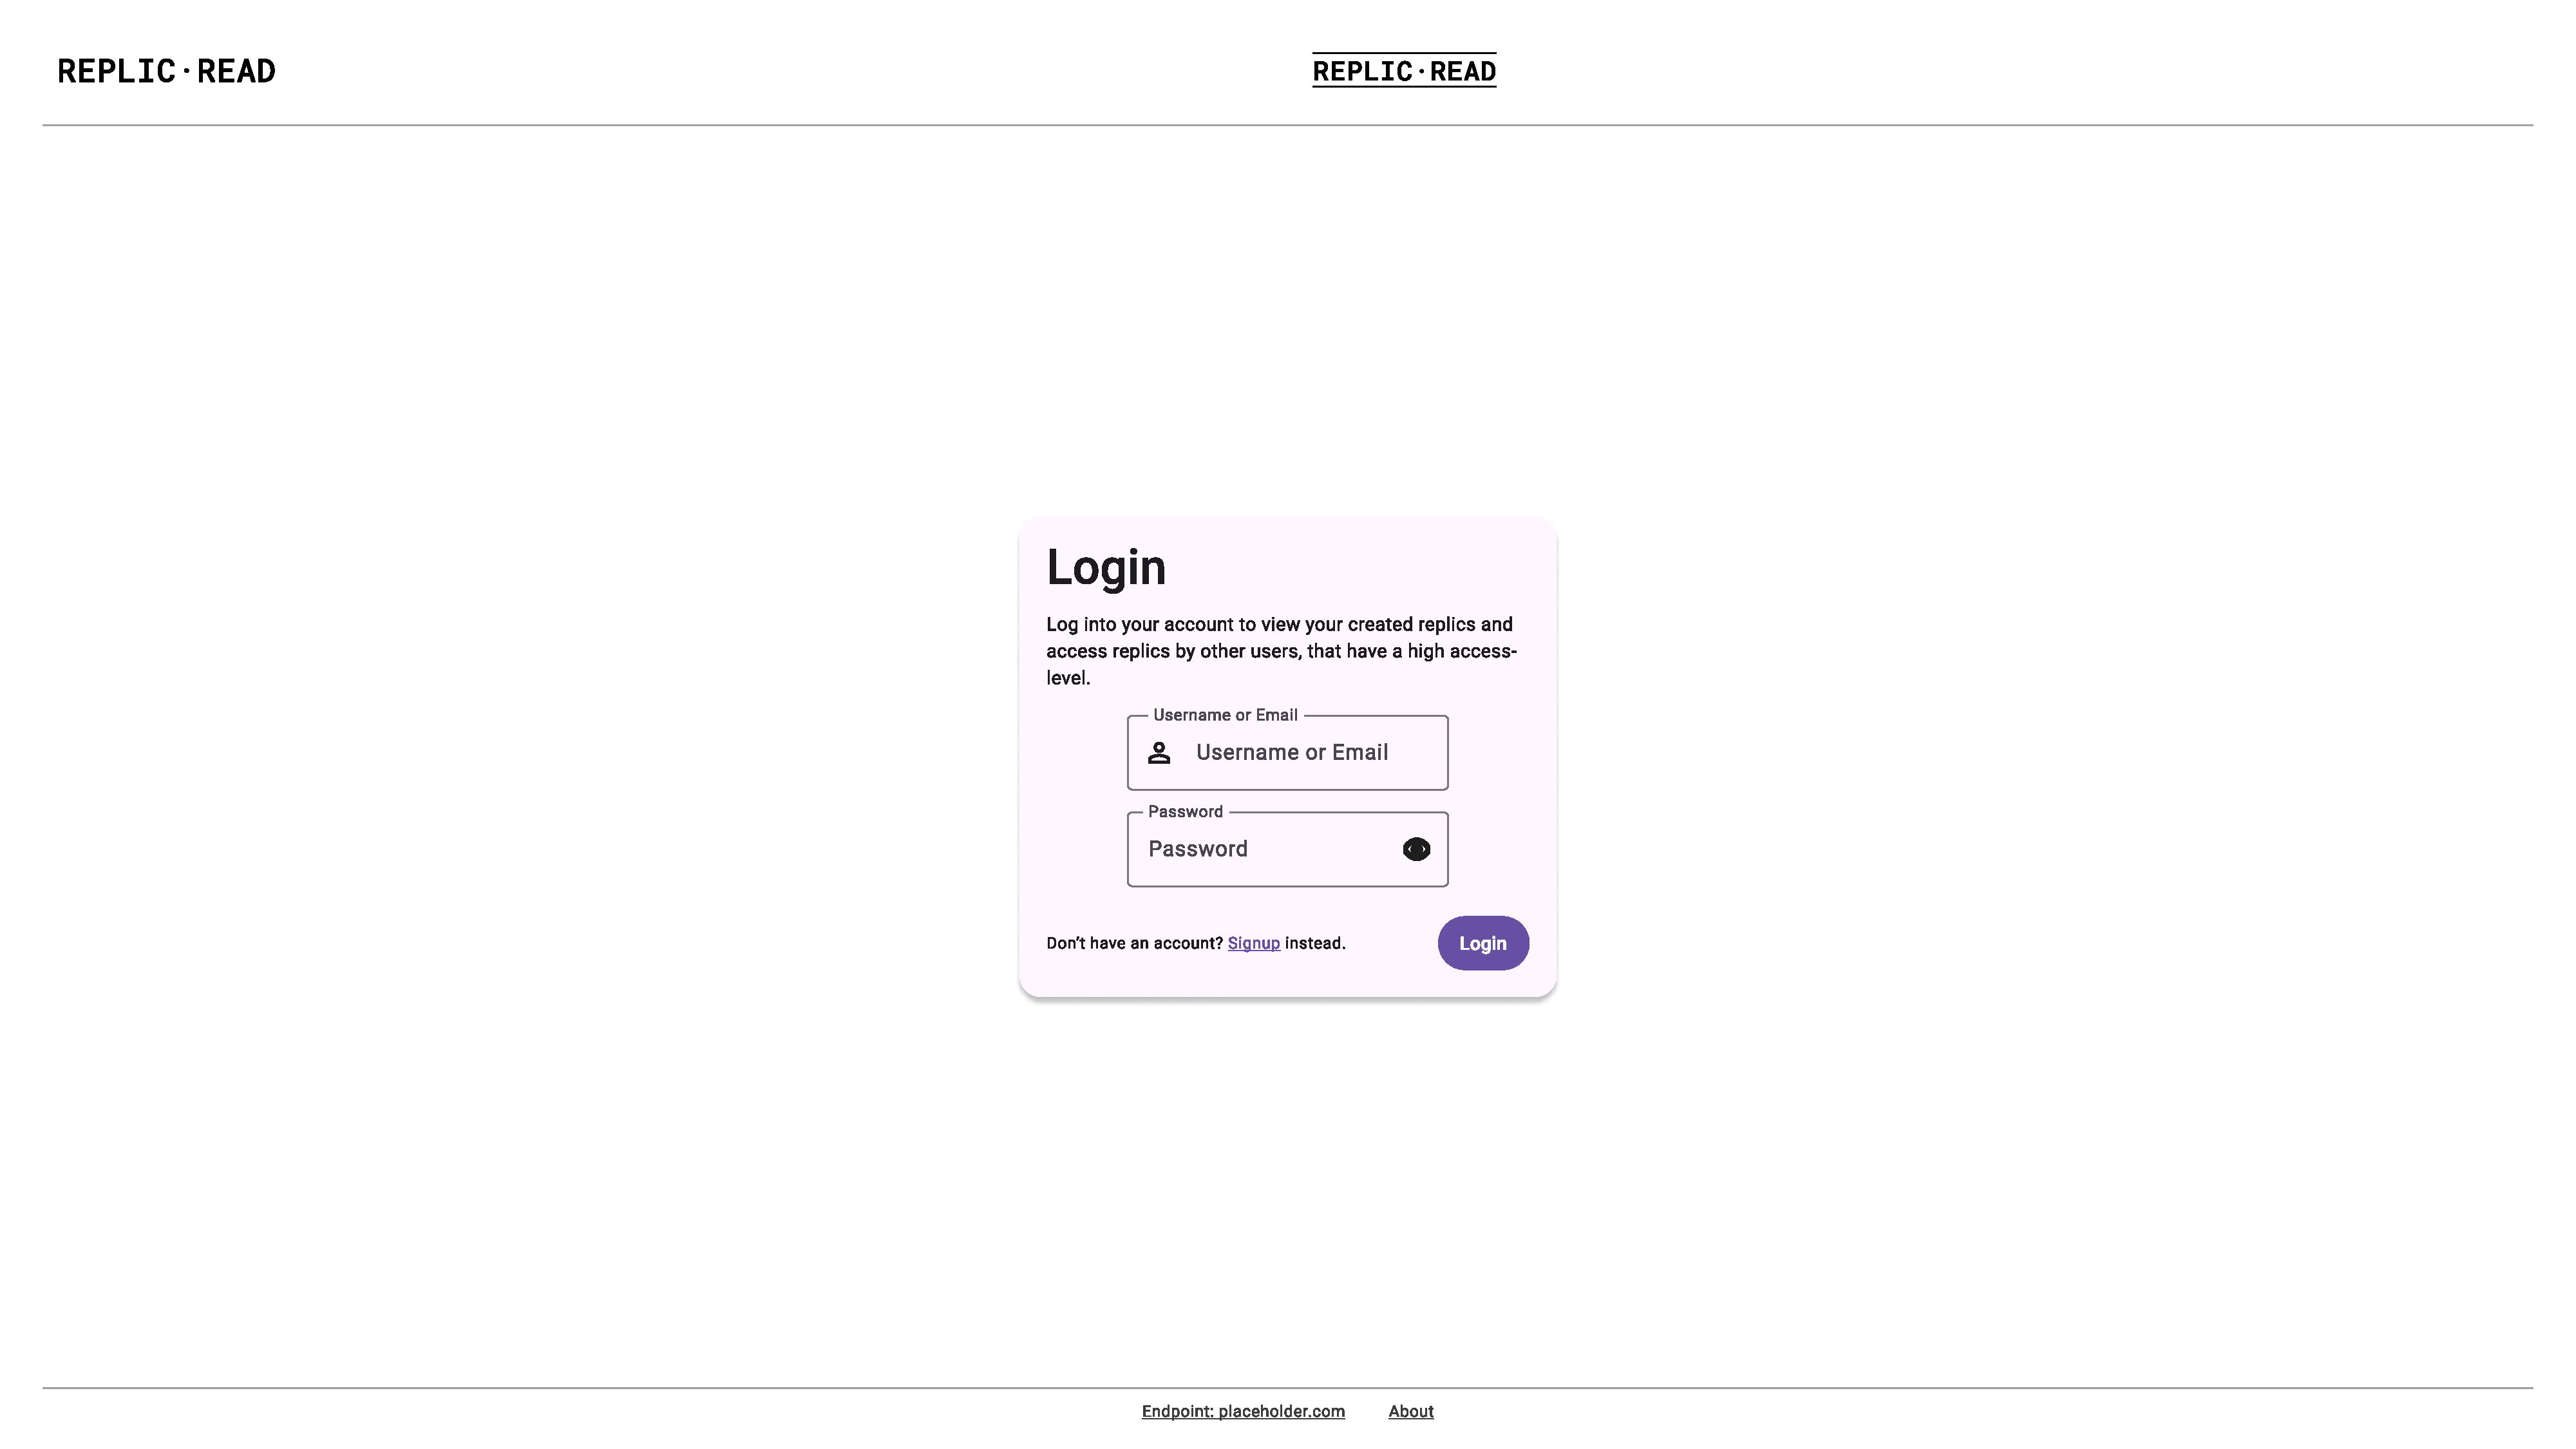
\includegraphics[width=12cm]{web-login}}

    \caption{Login view}
    \label{fig:web-login-view}
\end{figure}

\subsubsection{Signup View}
The signup screen (\ref{fig:web-signup-view}) allows the user to signup (\ref{subsubsec:signup}), or to navigate to the signup view (\ref{fig:web-login-view}) if an account already exists.
\begin{figure}
    \centering
    \fbox{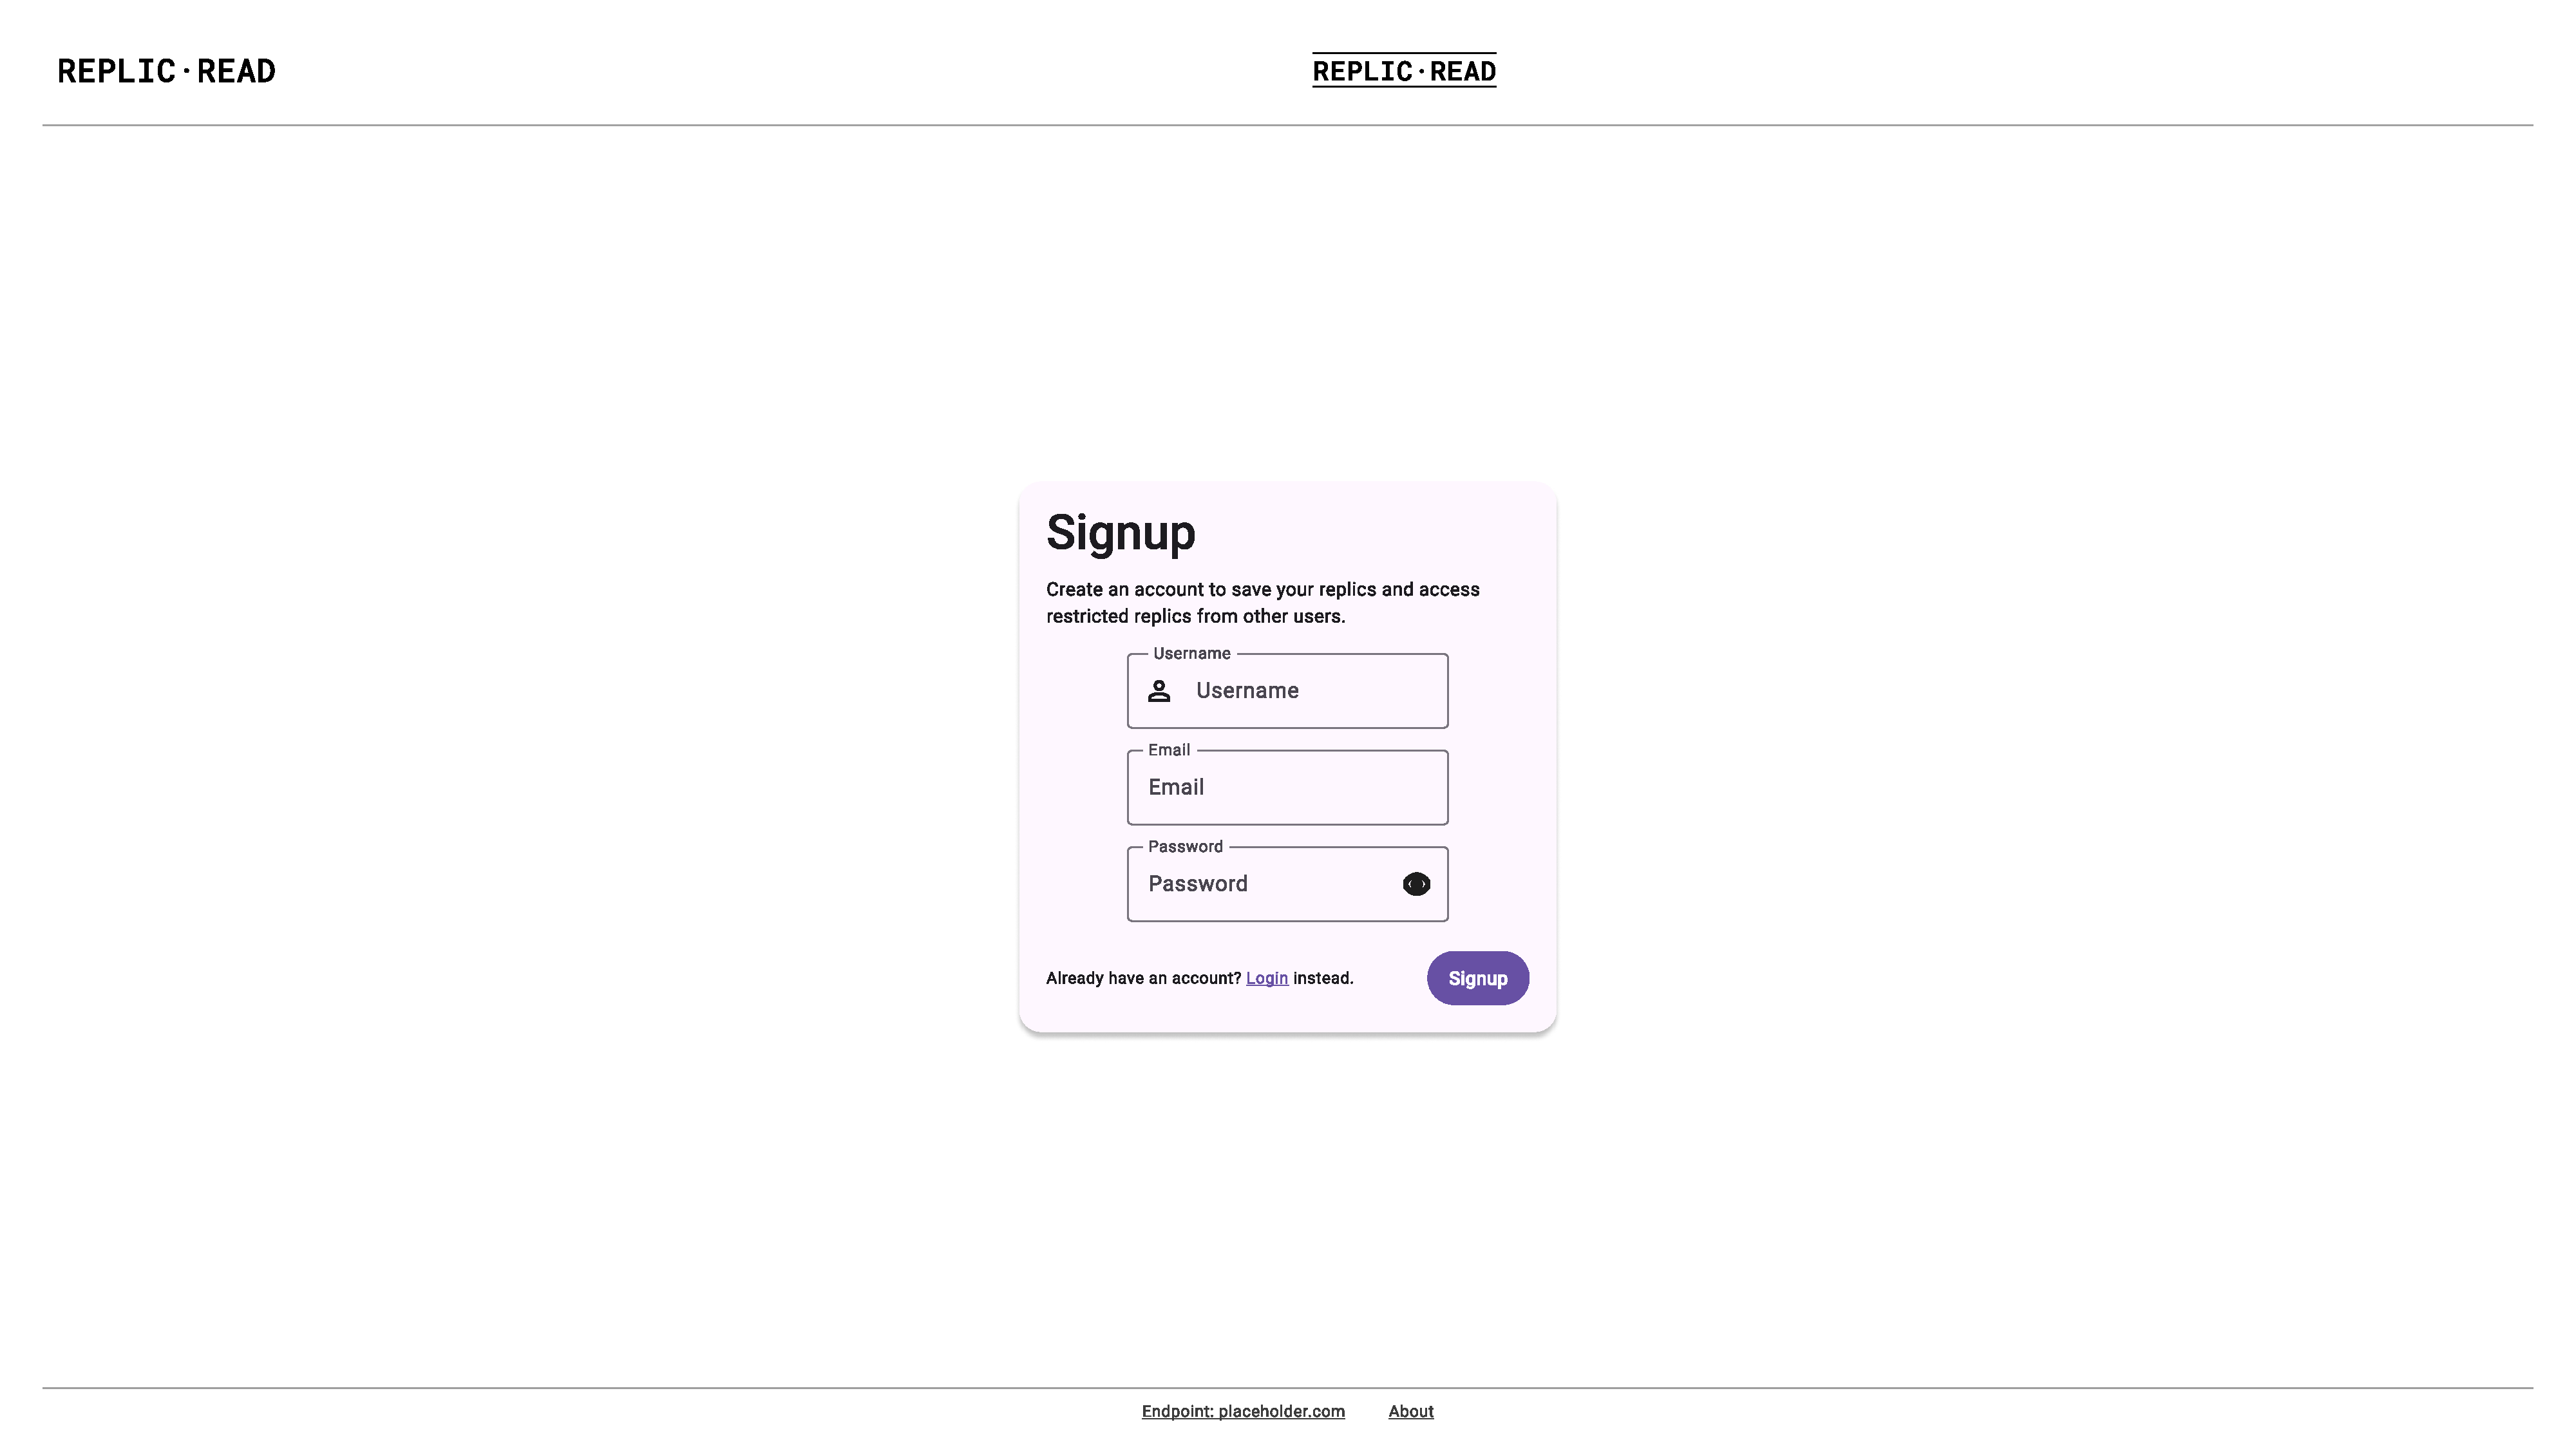
\includegraphics[width=12cm]{web-signup}}

    \caption{Signup view}
    \label{fig:web-signup-view}
\end{figure}

\subsubsection{Account View}
The account screen (\ref{fig:web-account-view}) shows basic information about the current account to the user.
Additionally, the user can change the username (\ref{subsubsec:change-username}), email (\ref{subsubsec:change-email}) and account color (\ref{subsubsec:change-color}).
A requested email-verification email can be cancelled.
\begin{figure}
    \centering
    \fbox{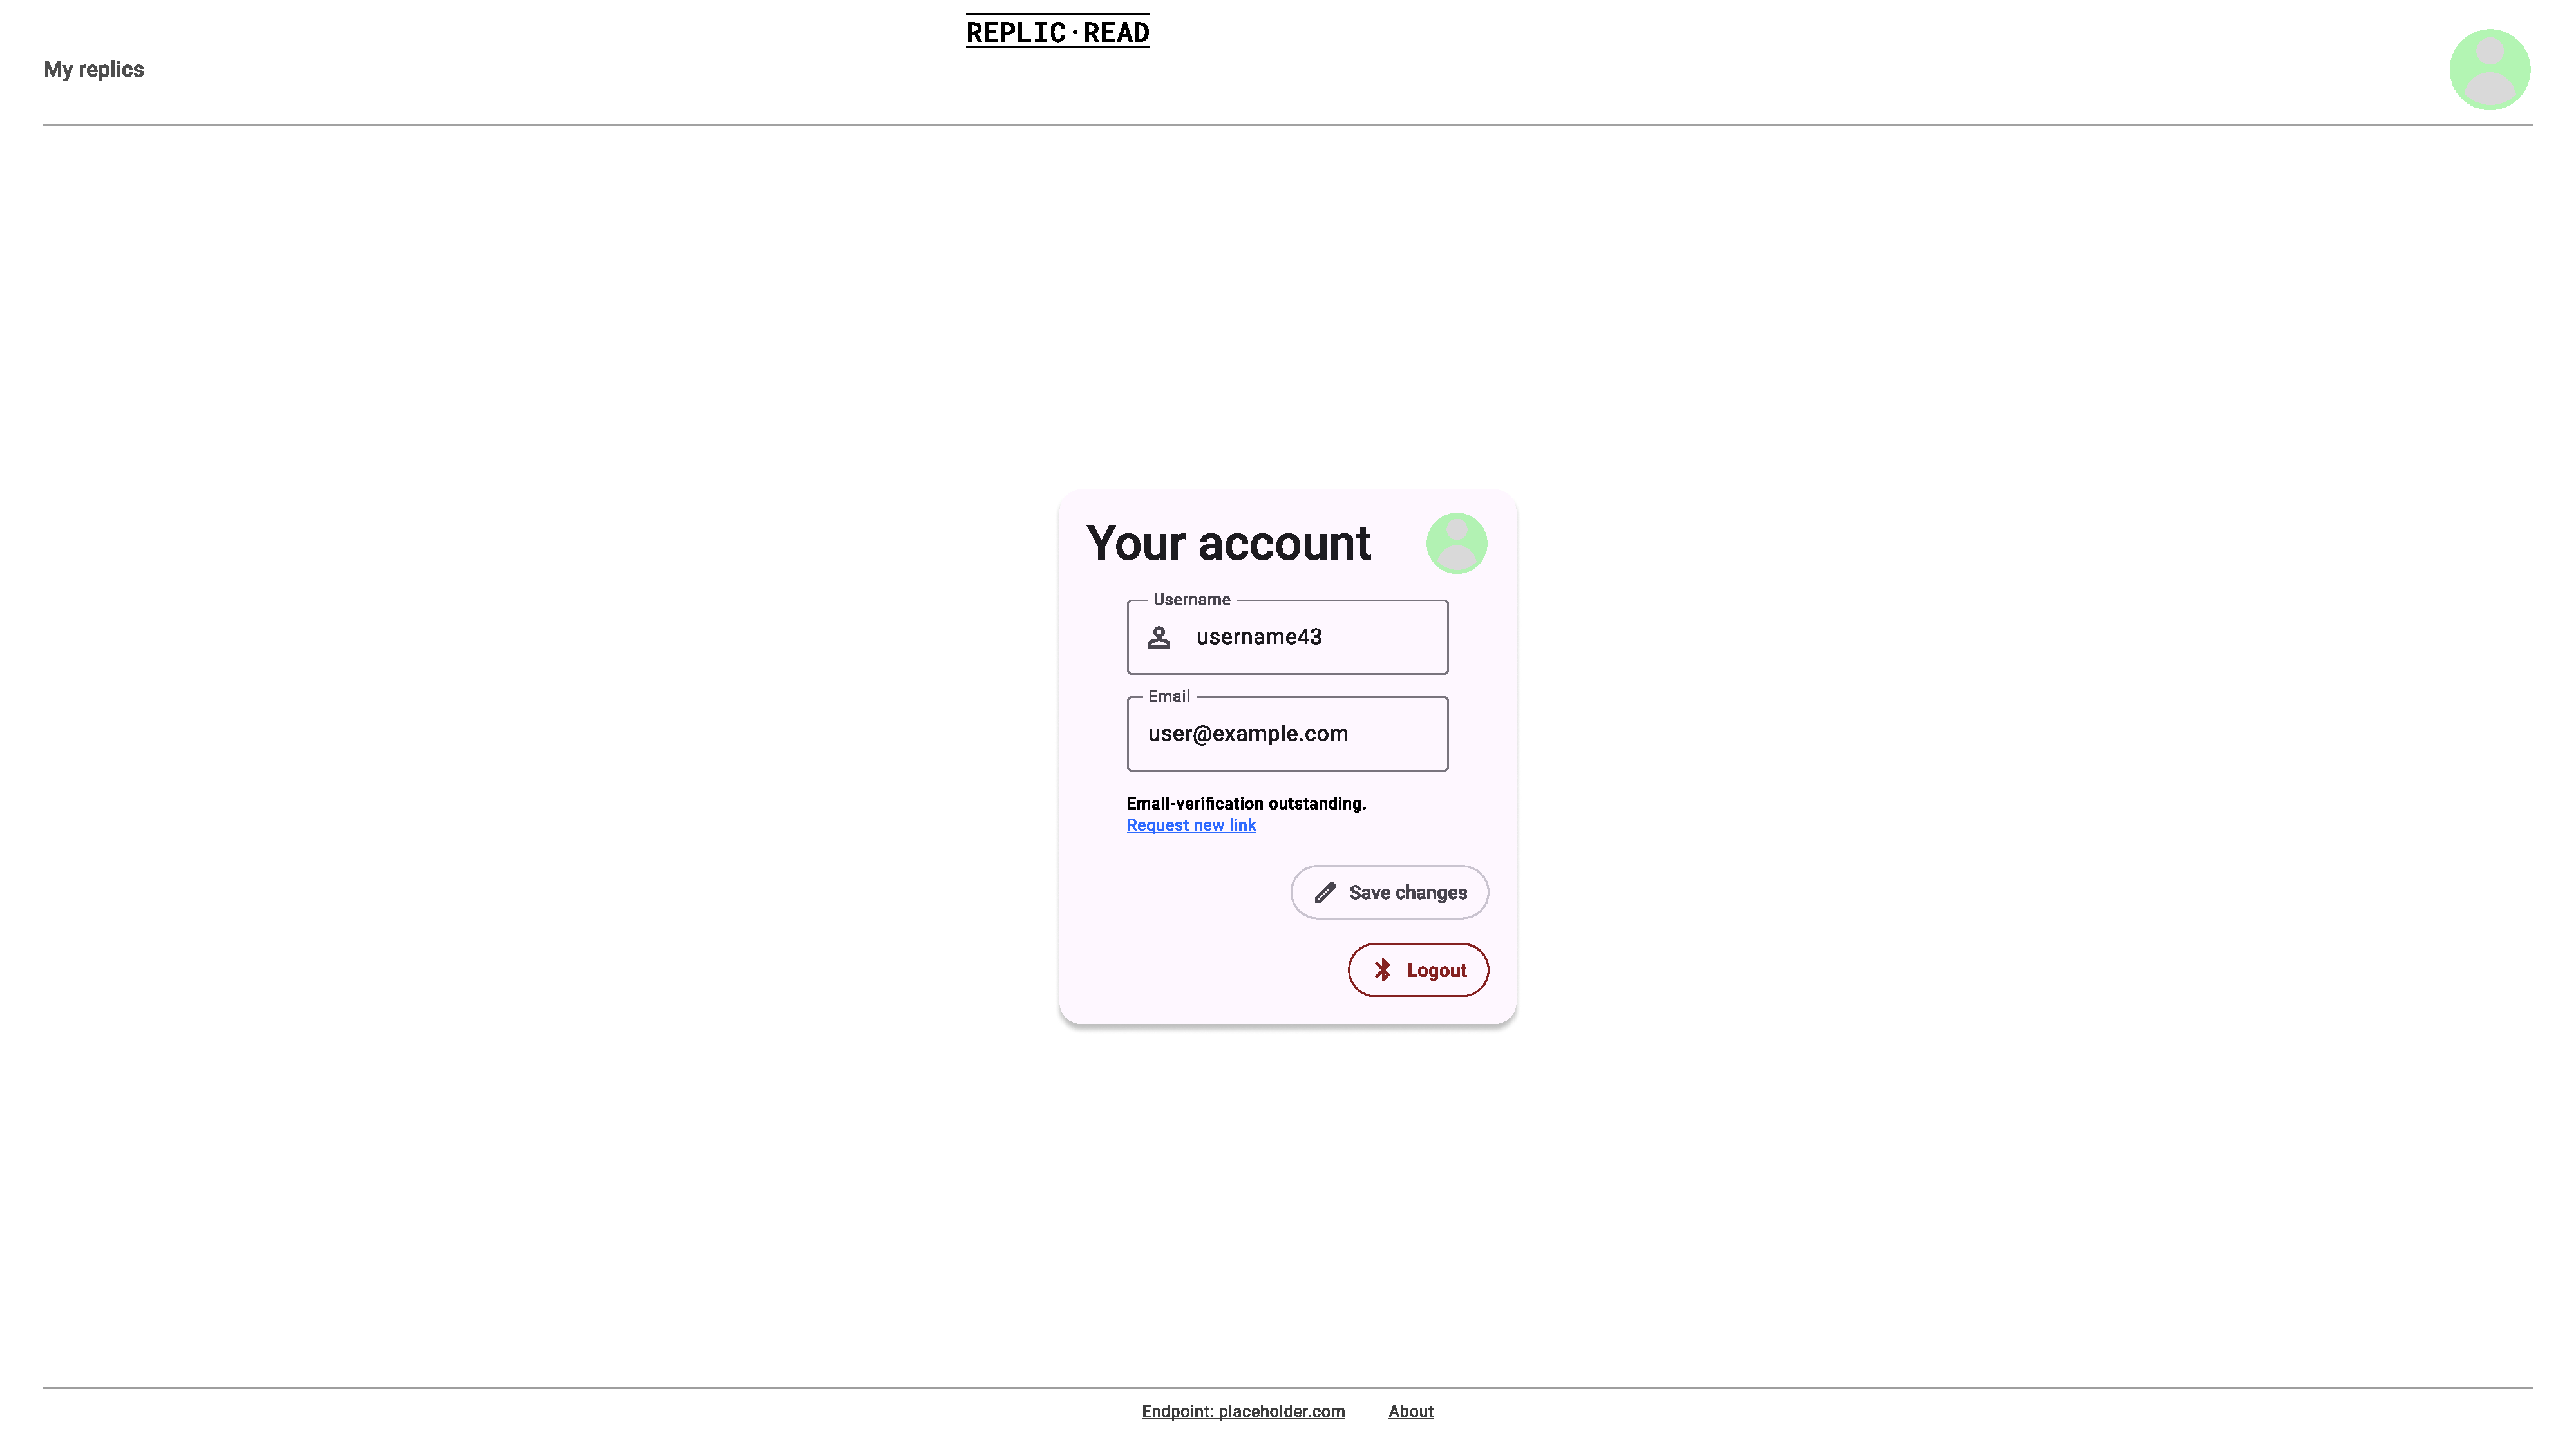
\includegraphics[width=12cm]{web-account}}

    \caption{Account view}
    \label{fig:web-account-view}
\end{figure}

\subsubsection{Admin config View}
The admin config view (\ref{fig:web-config-view}) allows the admin account to perform all the config changes that are available.
Additionally, there is a panel for an admin to create a user (\ref{subsubsec:create-user}).
\begin{figure}
    \centering
    \fbox{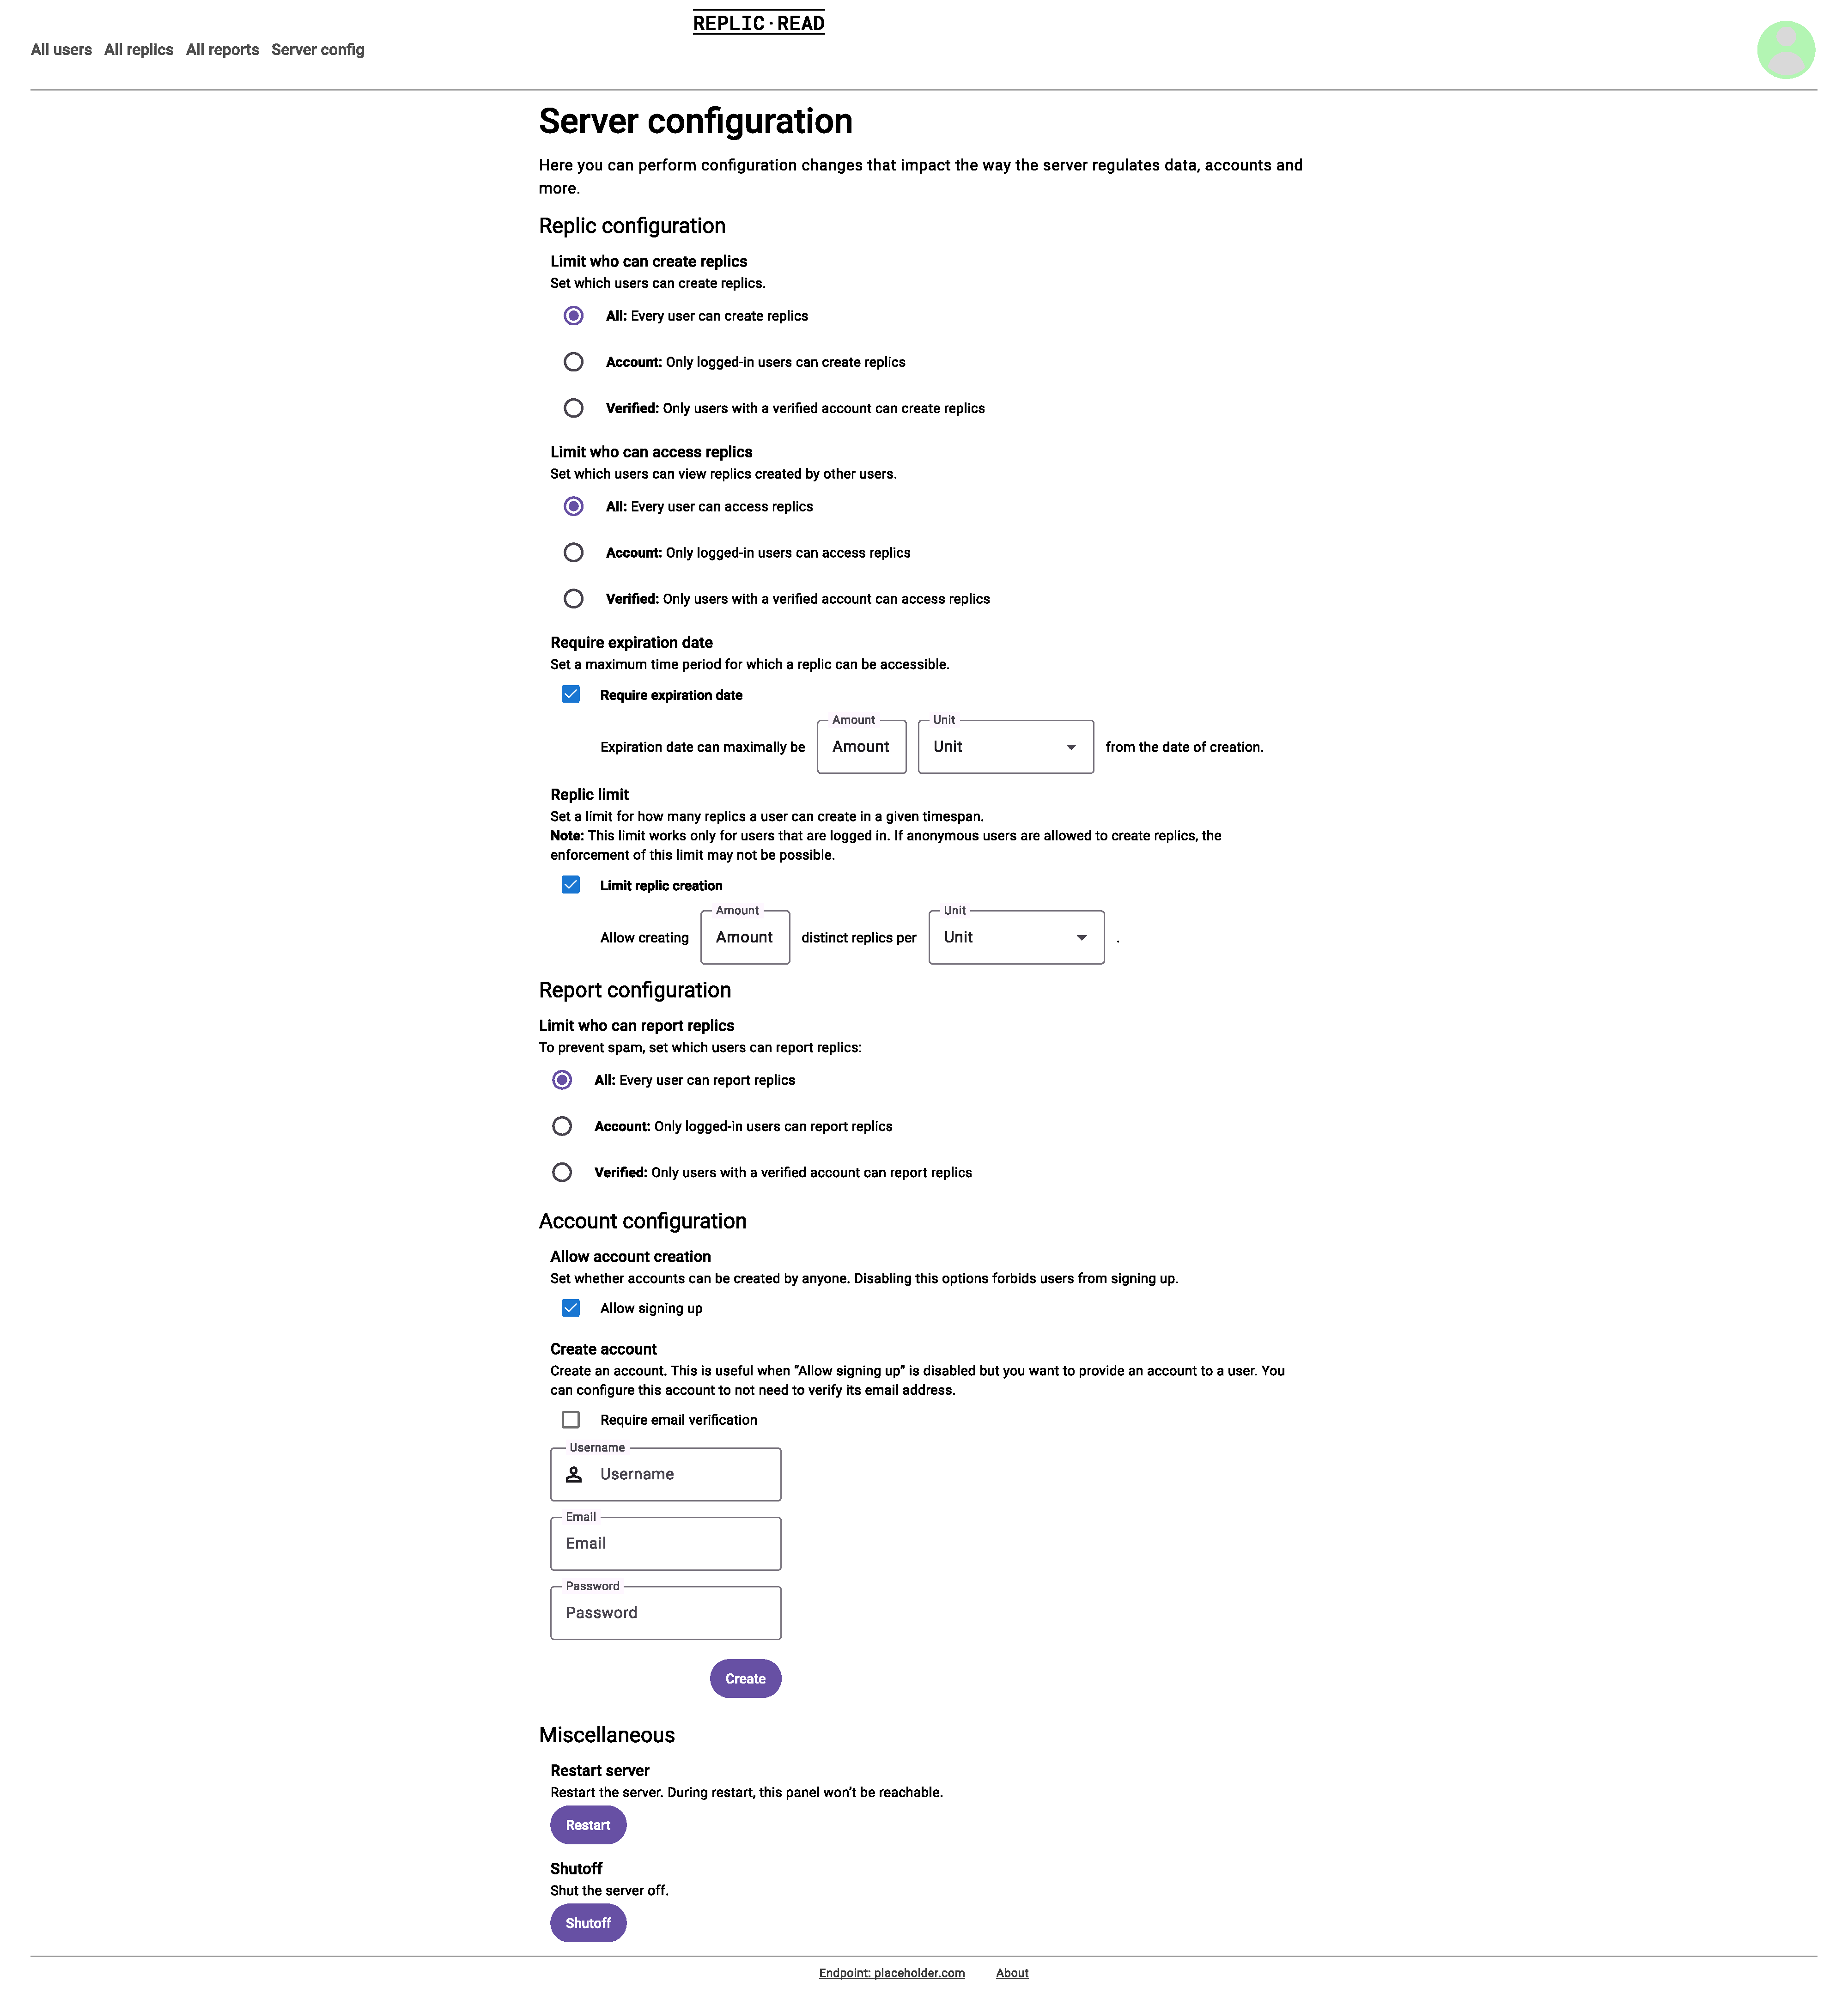
\includegraphics[width=12cm]{web-config}}

    \caption{Admin config view}
    \label{fig:web-config-view}
\end{figure}

\subsubsection{User replics view}
The user replics view gives a user an overview of the replics created by the account.
Each replic is represented by an item in a list that shows the original link, description, size, expiration date and state.
Each item has context actions that allow the user to deactivate (\ref{subsubsec:deactivate-replic}) or reactivate (\ref{subsubsec:reactivate-replic}) the replic.
The replics can be searched using a search bar, and filtered/sorted by using the sorting config that can be expanded (\ref{fig:web-user-replics-config-view}) or collapsed (\ref{fig:web-user-replics-noconfig-view}).
\begin{figure}
    \centering
    \fbox{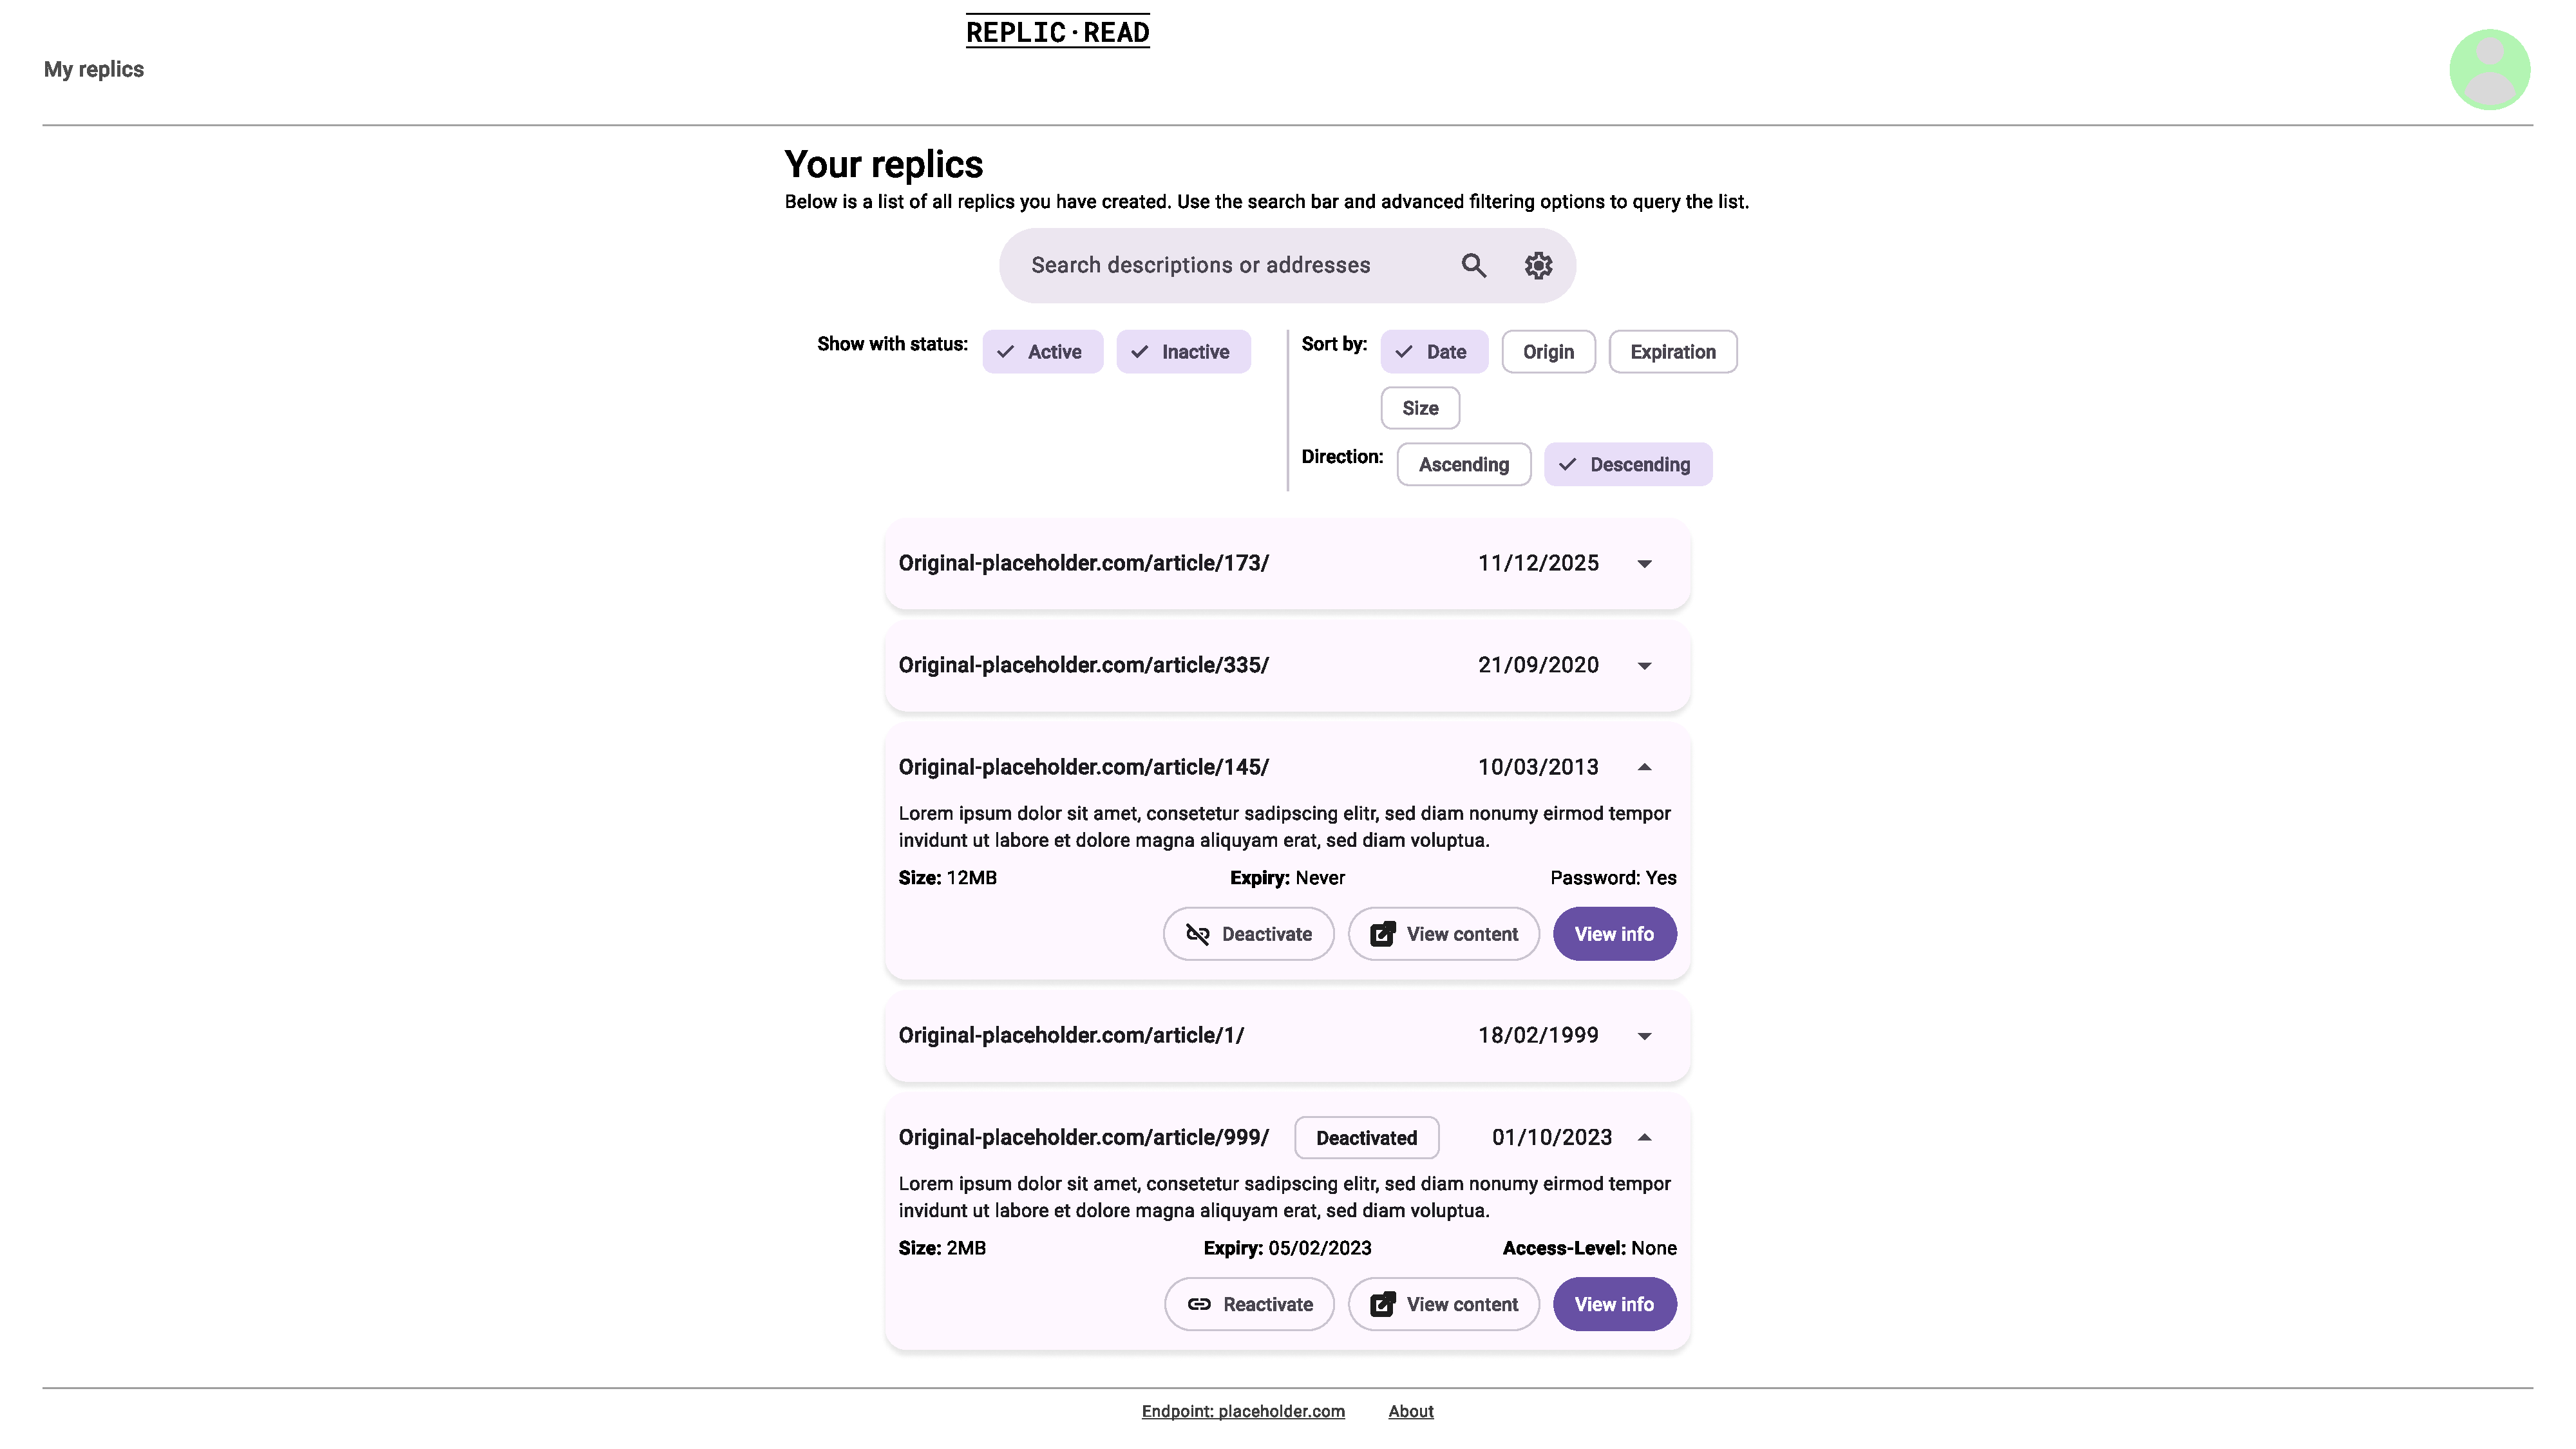
\includegraphics[width=12cm]{web-user-replics-config}}

    \caption{User replics view with search config visible}
    \label{fig:web-user-replics-config-view}
\end{figure}
\begin{figure}
    \centering
    \fbox{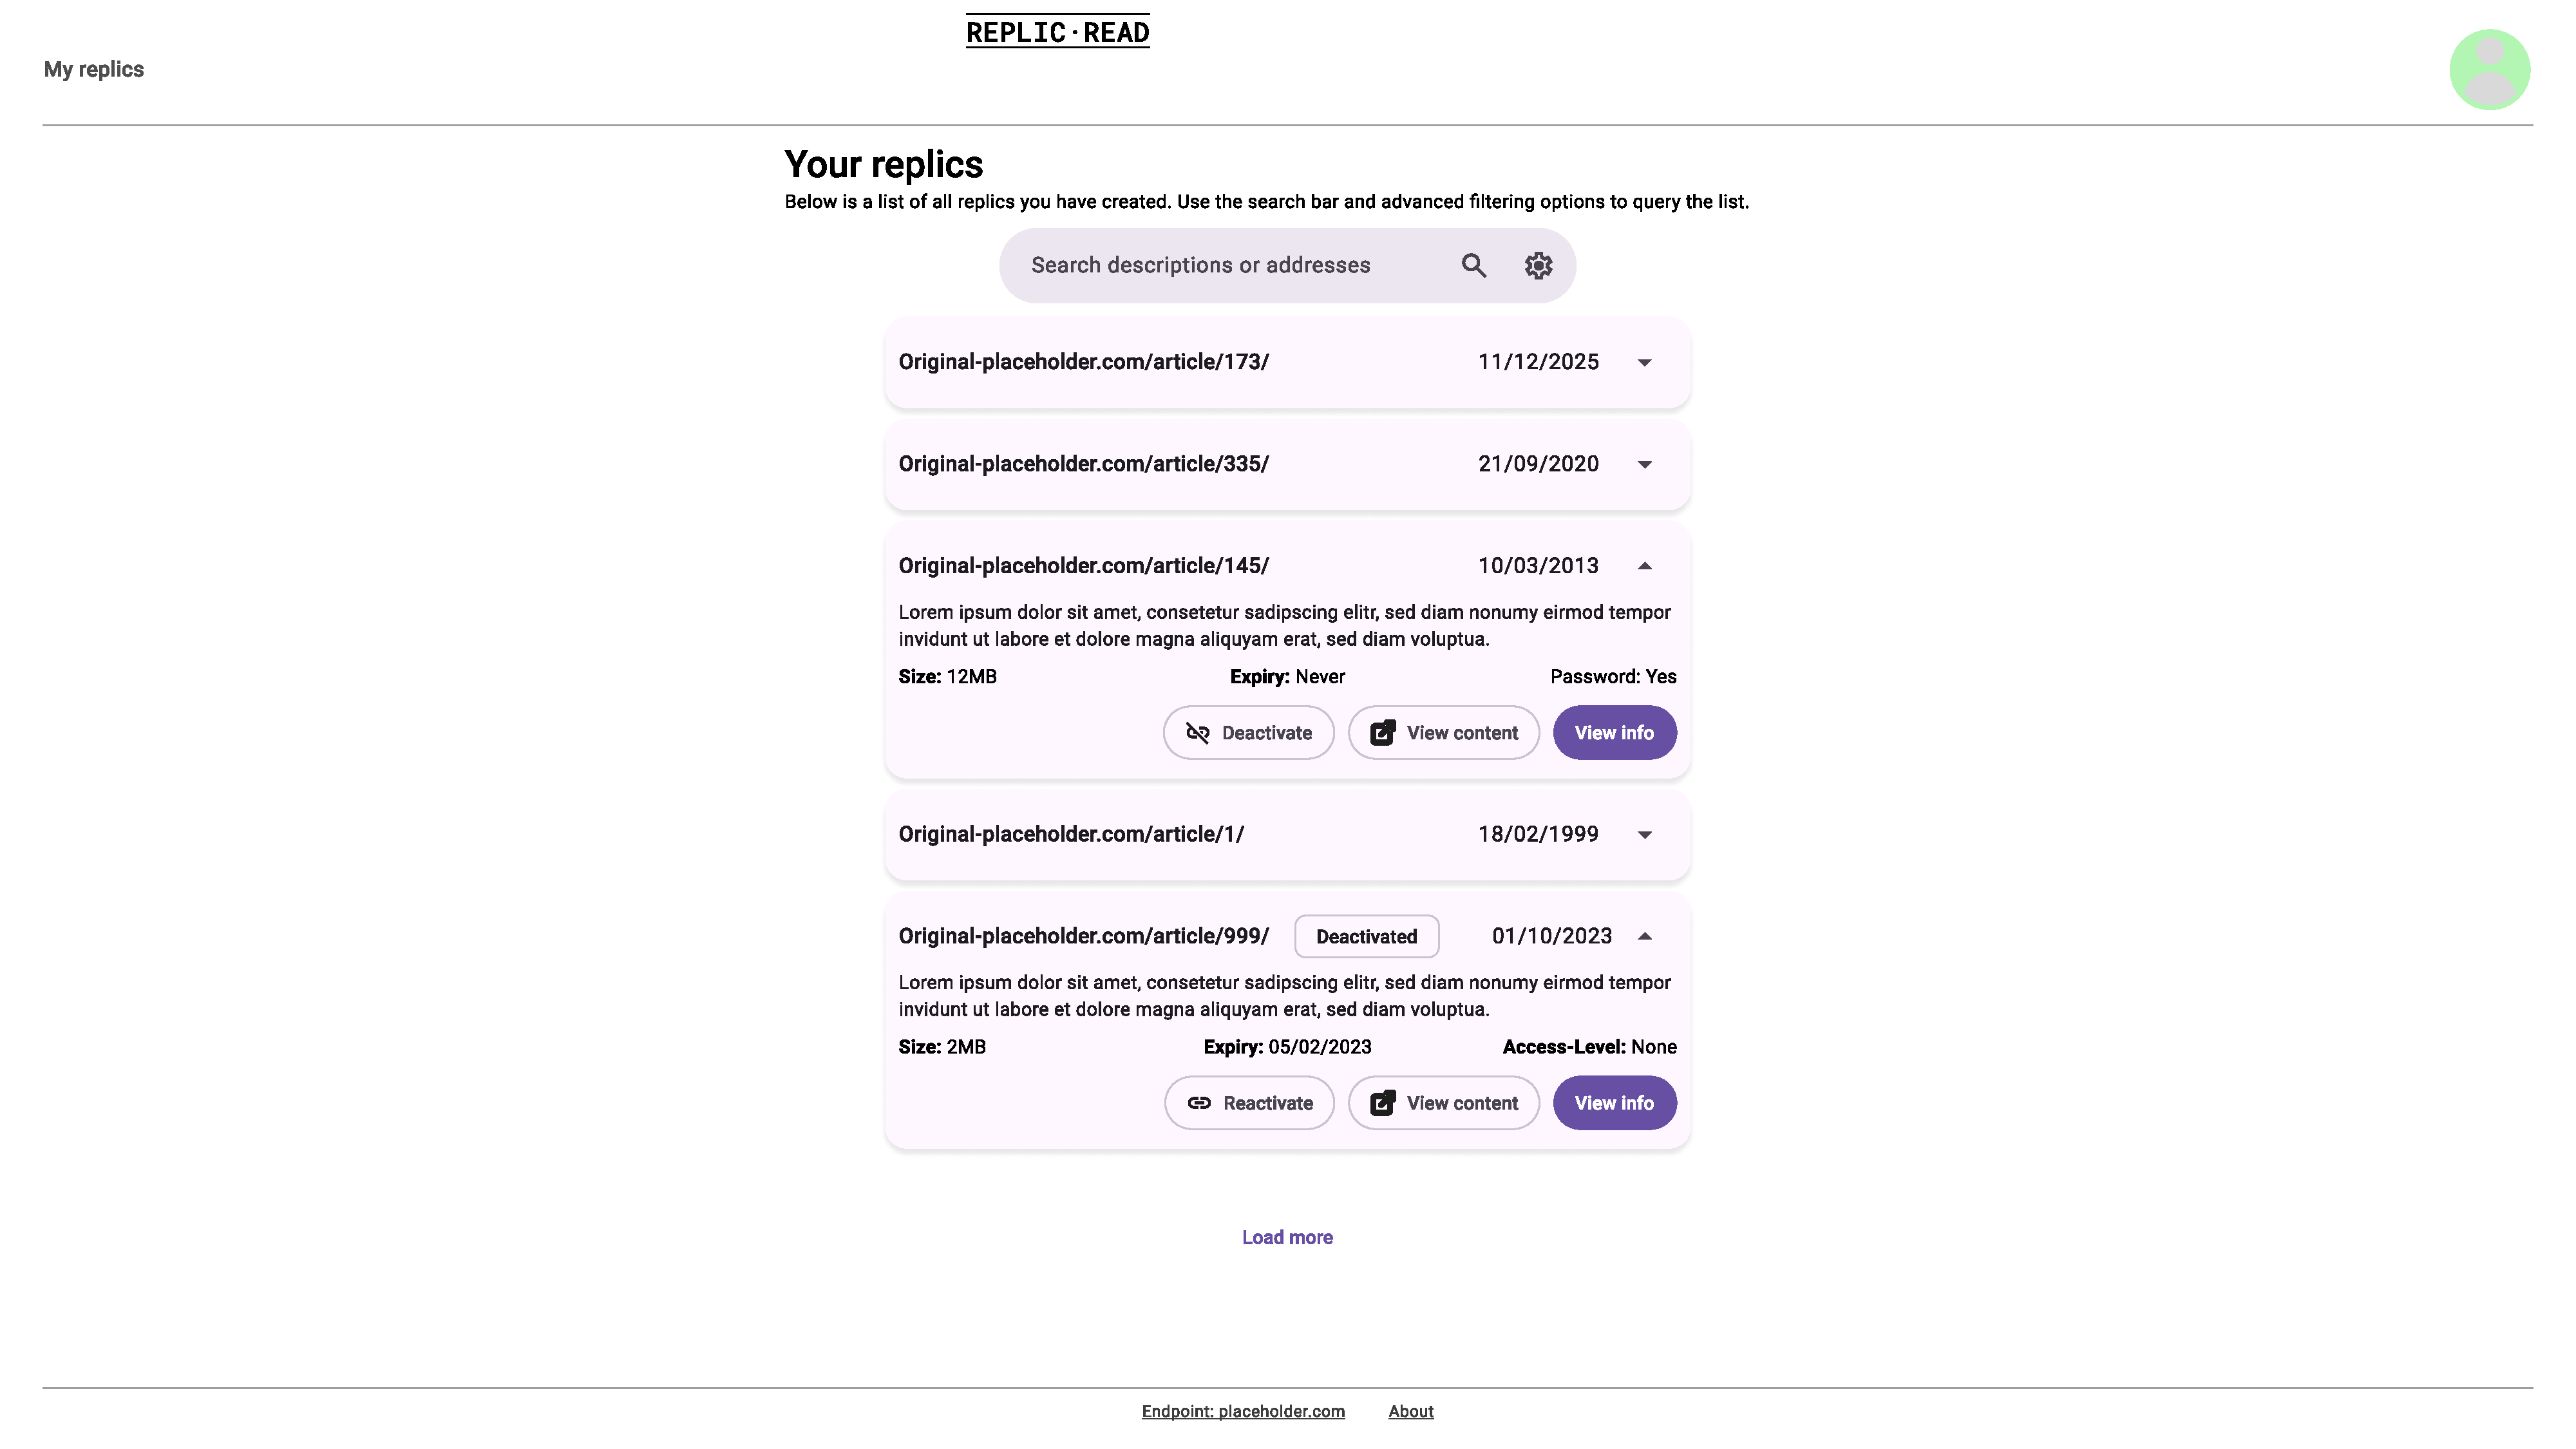
\includegraphics[width=12cm]{web-user-replics-noconfig}}

    \caption{User replics view}
    \label{fig:web-user-replics-noconfig-view}
\end{figure}

\subsubsection{Admin replics view}
The admin replics view allows the admin to view all replics created on the server.
Each replic is represented by an item in a list that shows the original link, description, size, expiration date and state.
Each item has config actions that allows the admin to remove (\ref{subsubsec:remove-replic}) or restore a replic.
The replics can be searched using a search bar, and filtered/sorted by using the sorting config that can be expanded (\ref{fig:web-admin-replics-config-view}) or collapsed (\ref{fig:web-admin-replics-noconfig-view}).
A dropdown to filter the replics by authoring user is also available.
\begin{figure}
    \centering
    \fbox{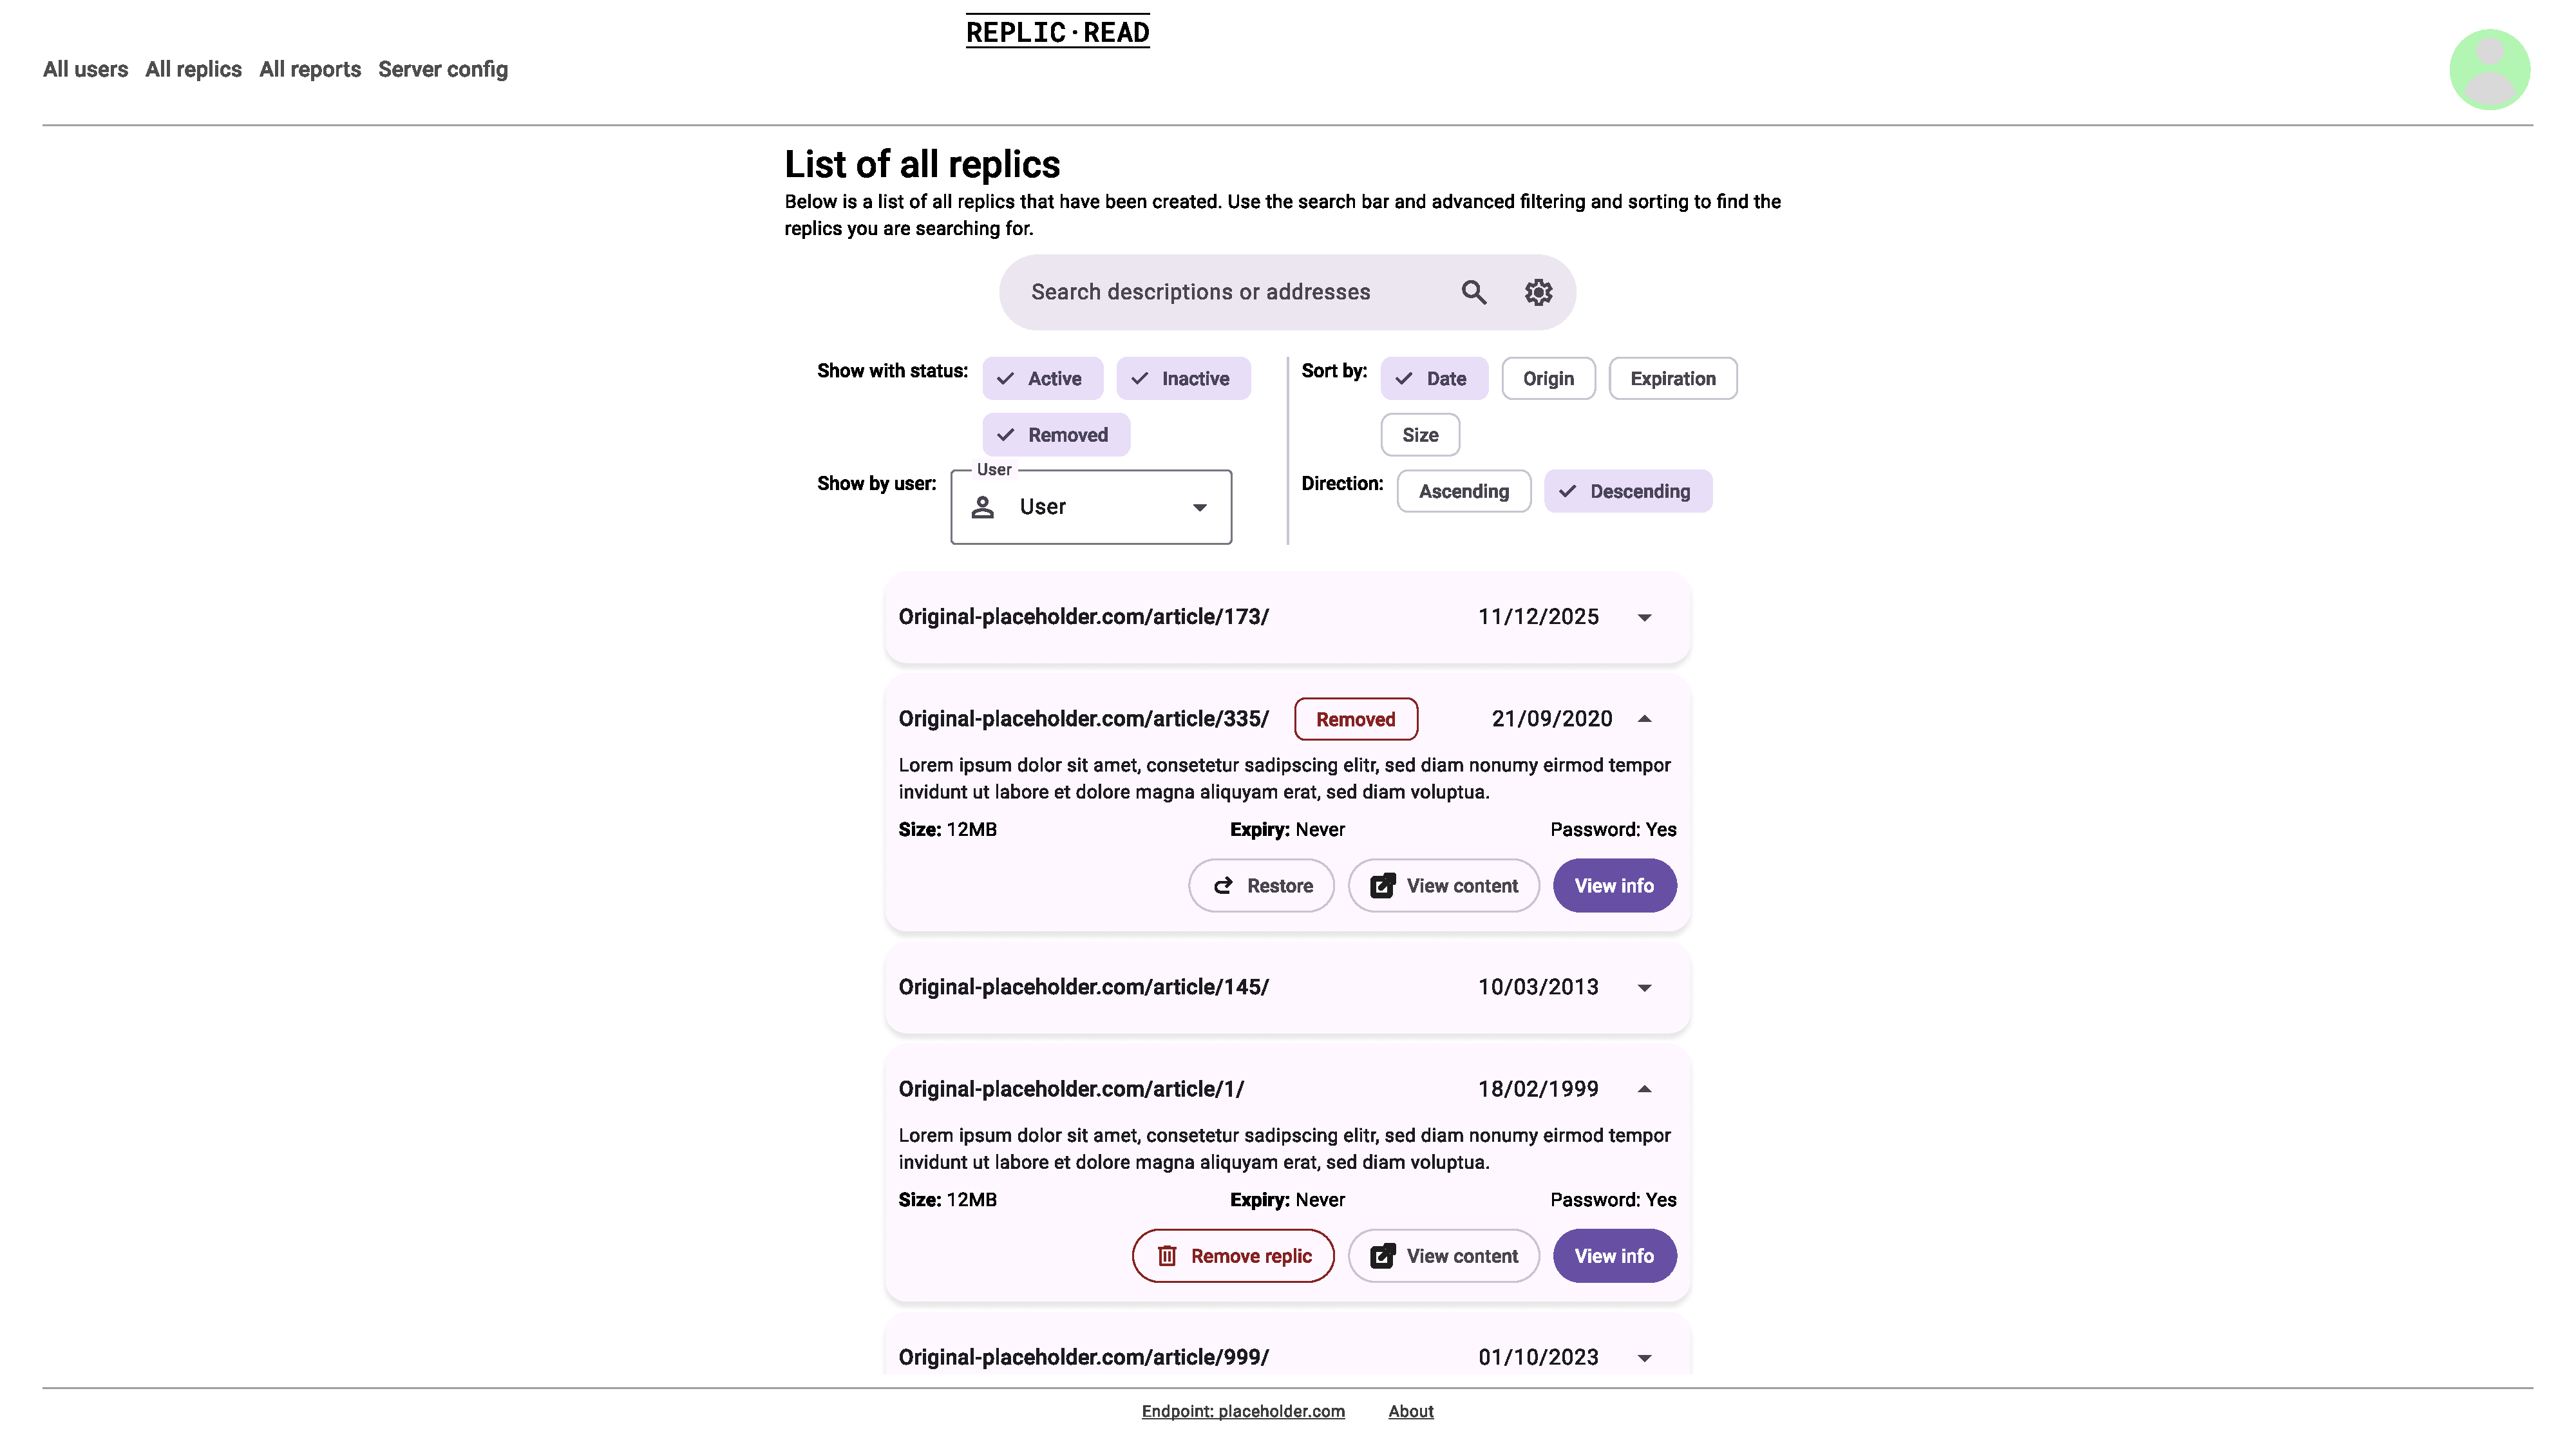
\includegraphics[width=12cm]{web-admin-replics-config}}

    \caption{Admin replics view with search config visible}
    \label{fig:web-admin-replics-config-view}
\end{figure}
\begin{figure}
    \centering
    \fbox{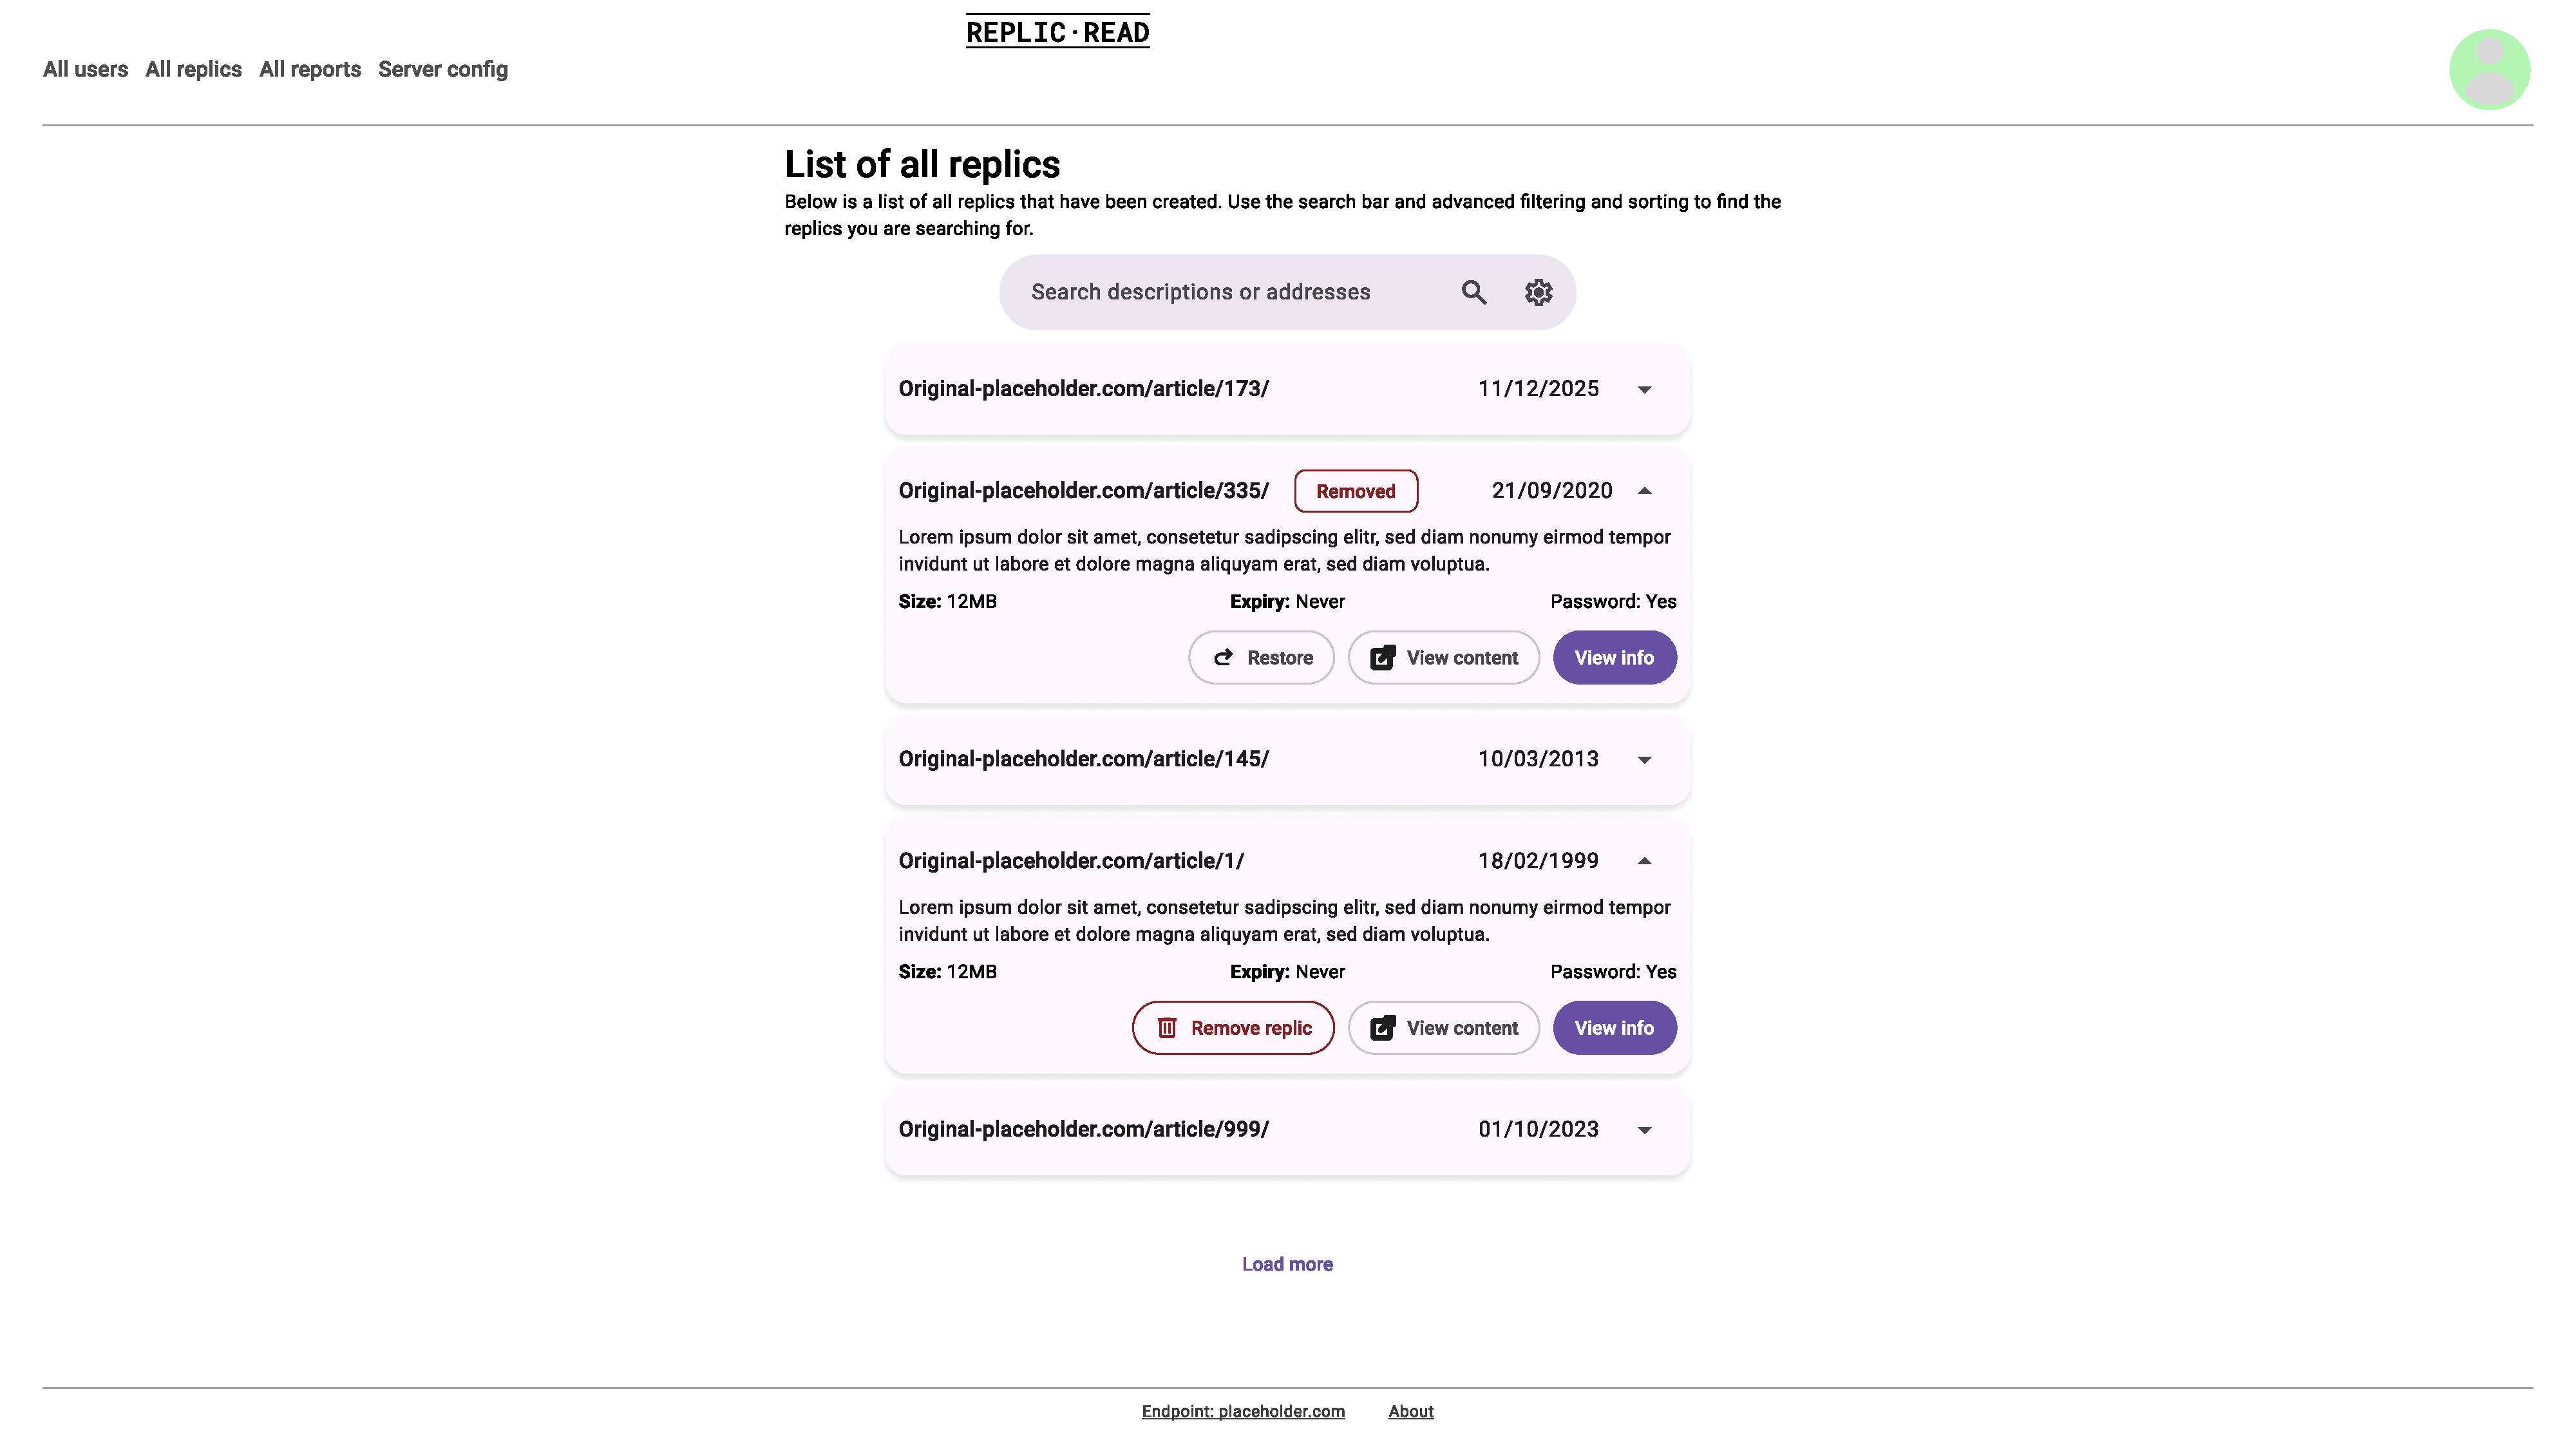
\includegraphics[width=12cm]{web-admin-replics-noconfig}}

    \caption{Admin replics view}
    \label{fig:web-admin-replics-noconfig-view}
\end{figure}

\subsubsection{Admin accounts view}
The admin accounts view allows the admin to view all accounts on the server.
Each account is represented by an item in a list that shows the username, profile color and email-address.
Each item has context actions that allow the admin to deactivate (\ref{subsubsec:deactivate-acc-admin}) or reactivate (\ref{subsubsec:reactivate-acc-admin}) an account, and to reset an account's password (\ref{subsubsec:reset-pass}).
The accounts can be searched using a search bar, and filtered/sorted by using the sorting config that can be expanded (\ref{fig:web-accounts-config-view}) or collapsed (\ref{fig:web-accounts-noconfig-view}).
\begin{figure}
    \centering
    \fbox{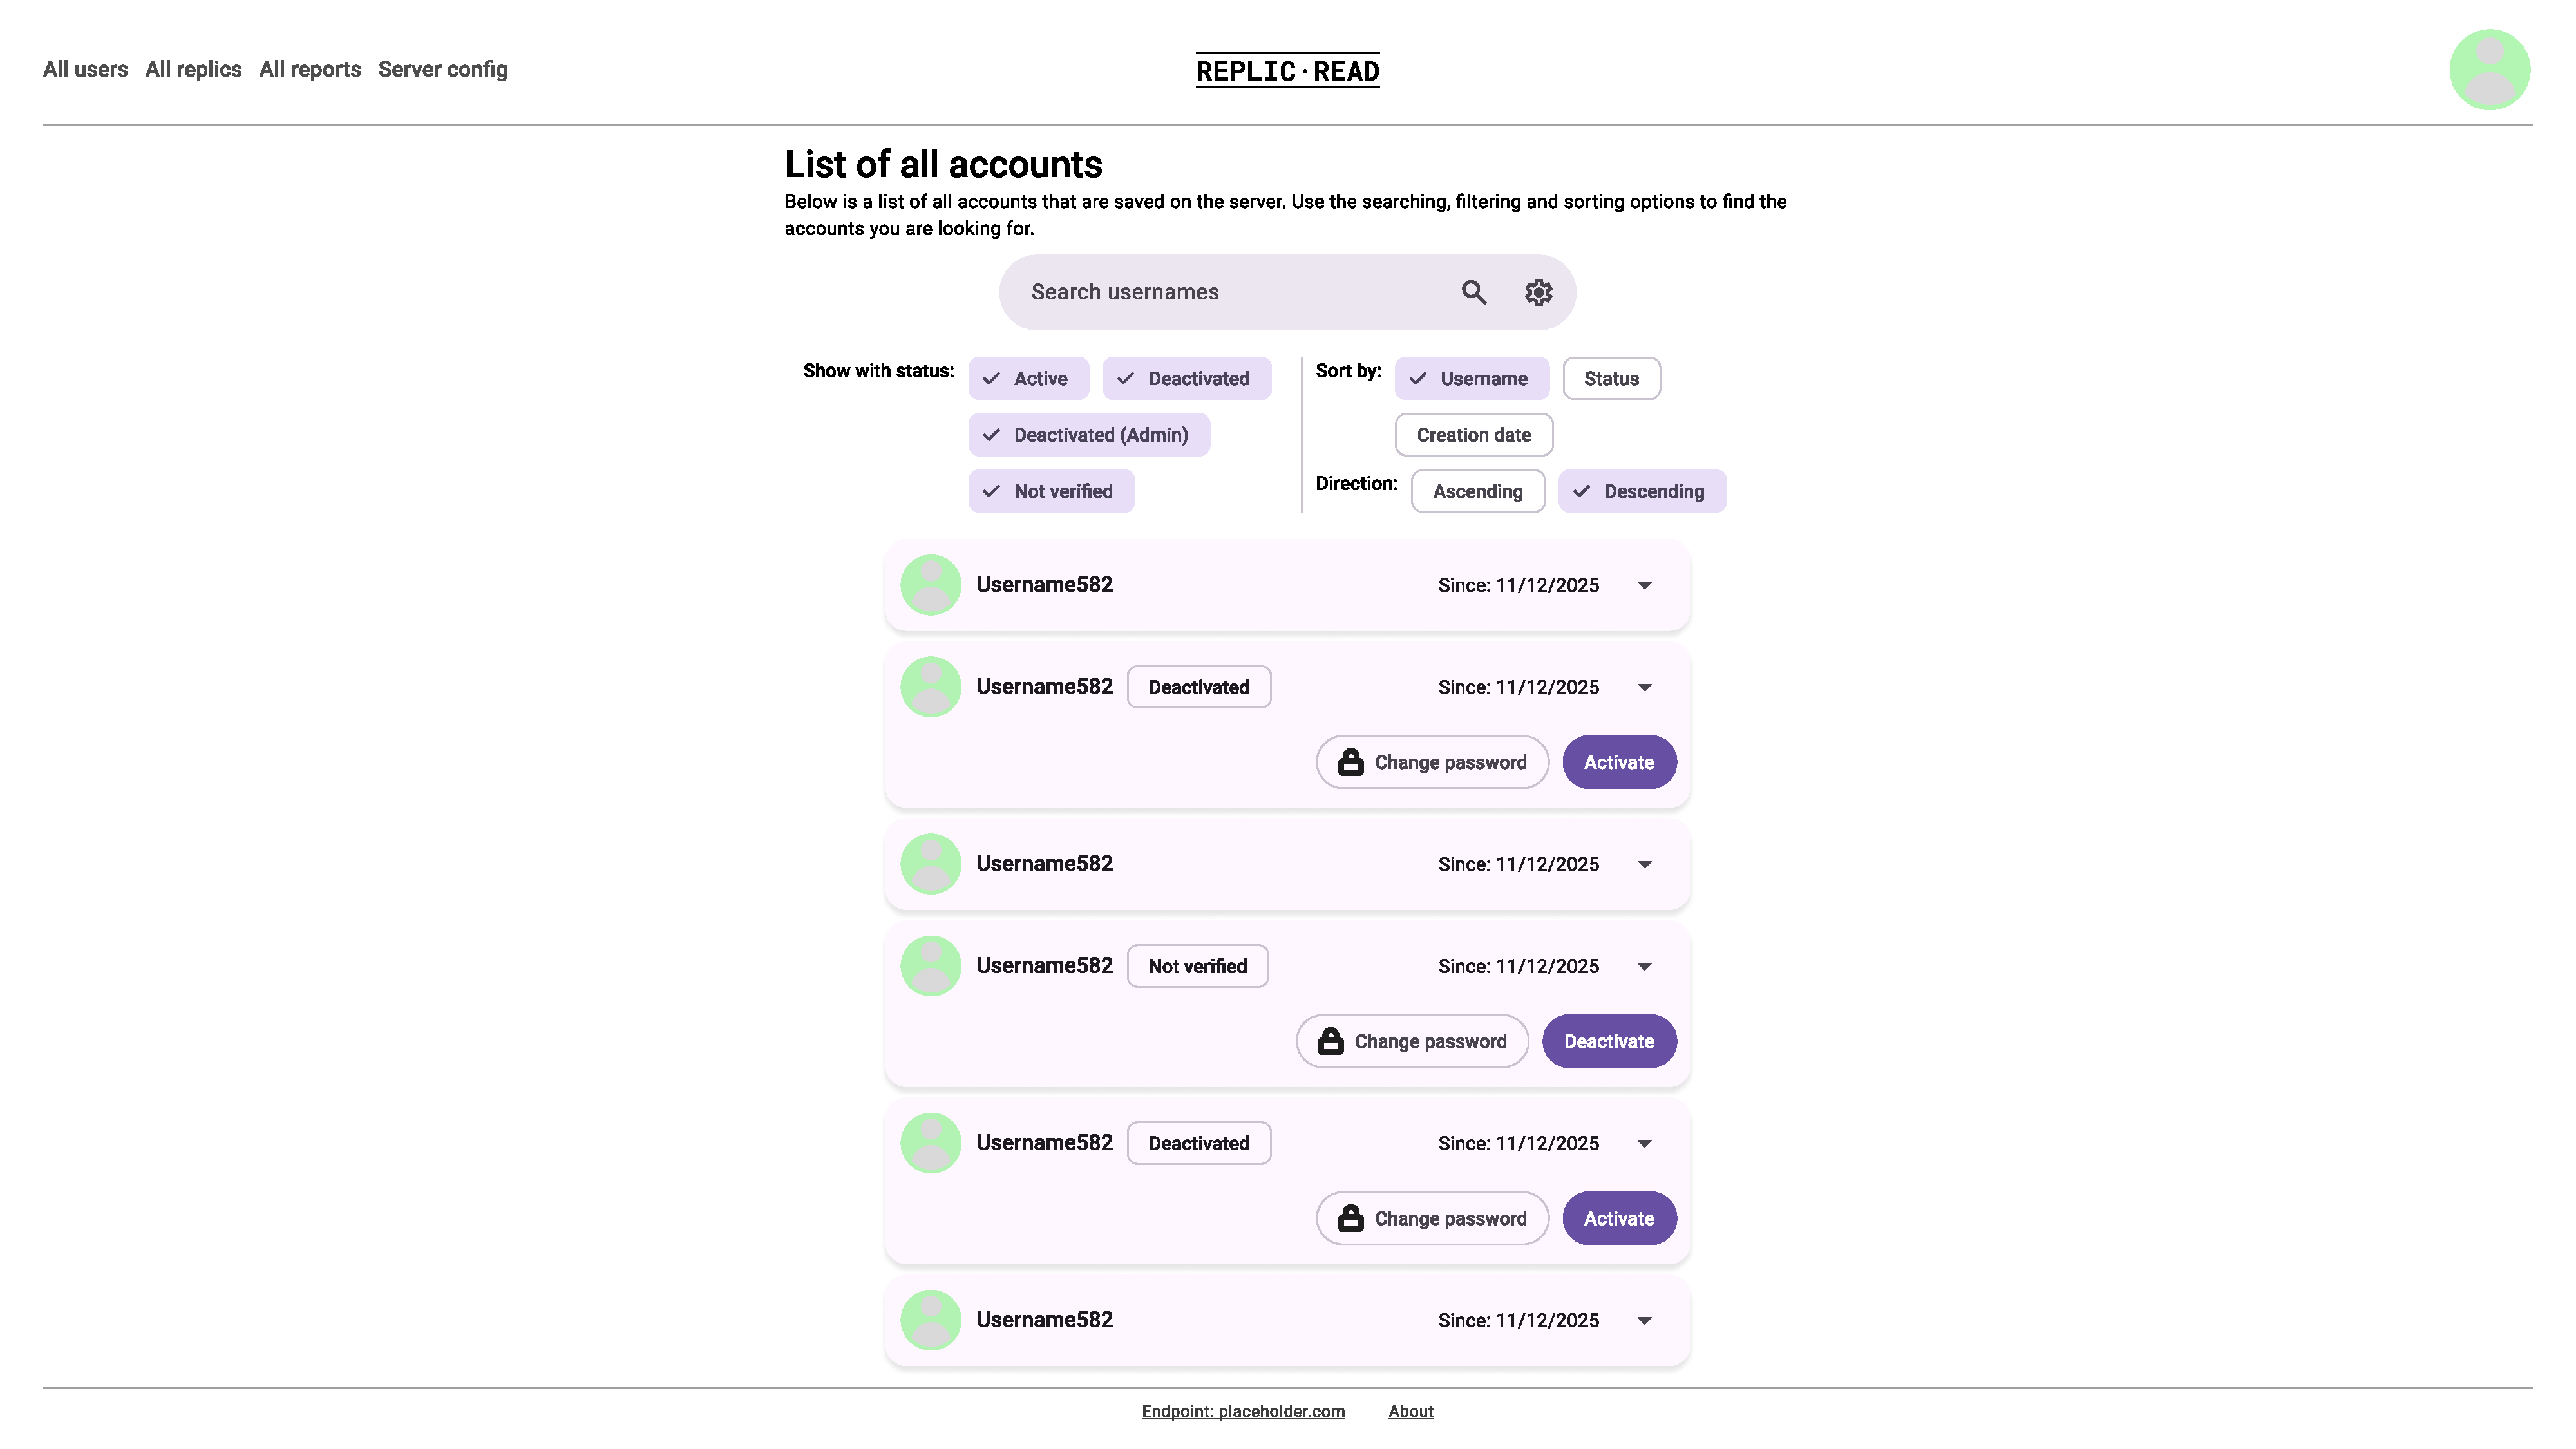
\includegraphics[width=12cm]{web-accounts-config}}

    \caption{Admin accounts view with search config visible}
    \label{fig:web-accounts-config-view}
\end{figure}
\begin{figure}
    \centering
    \fbox{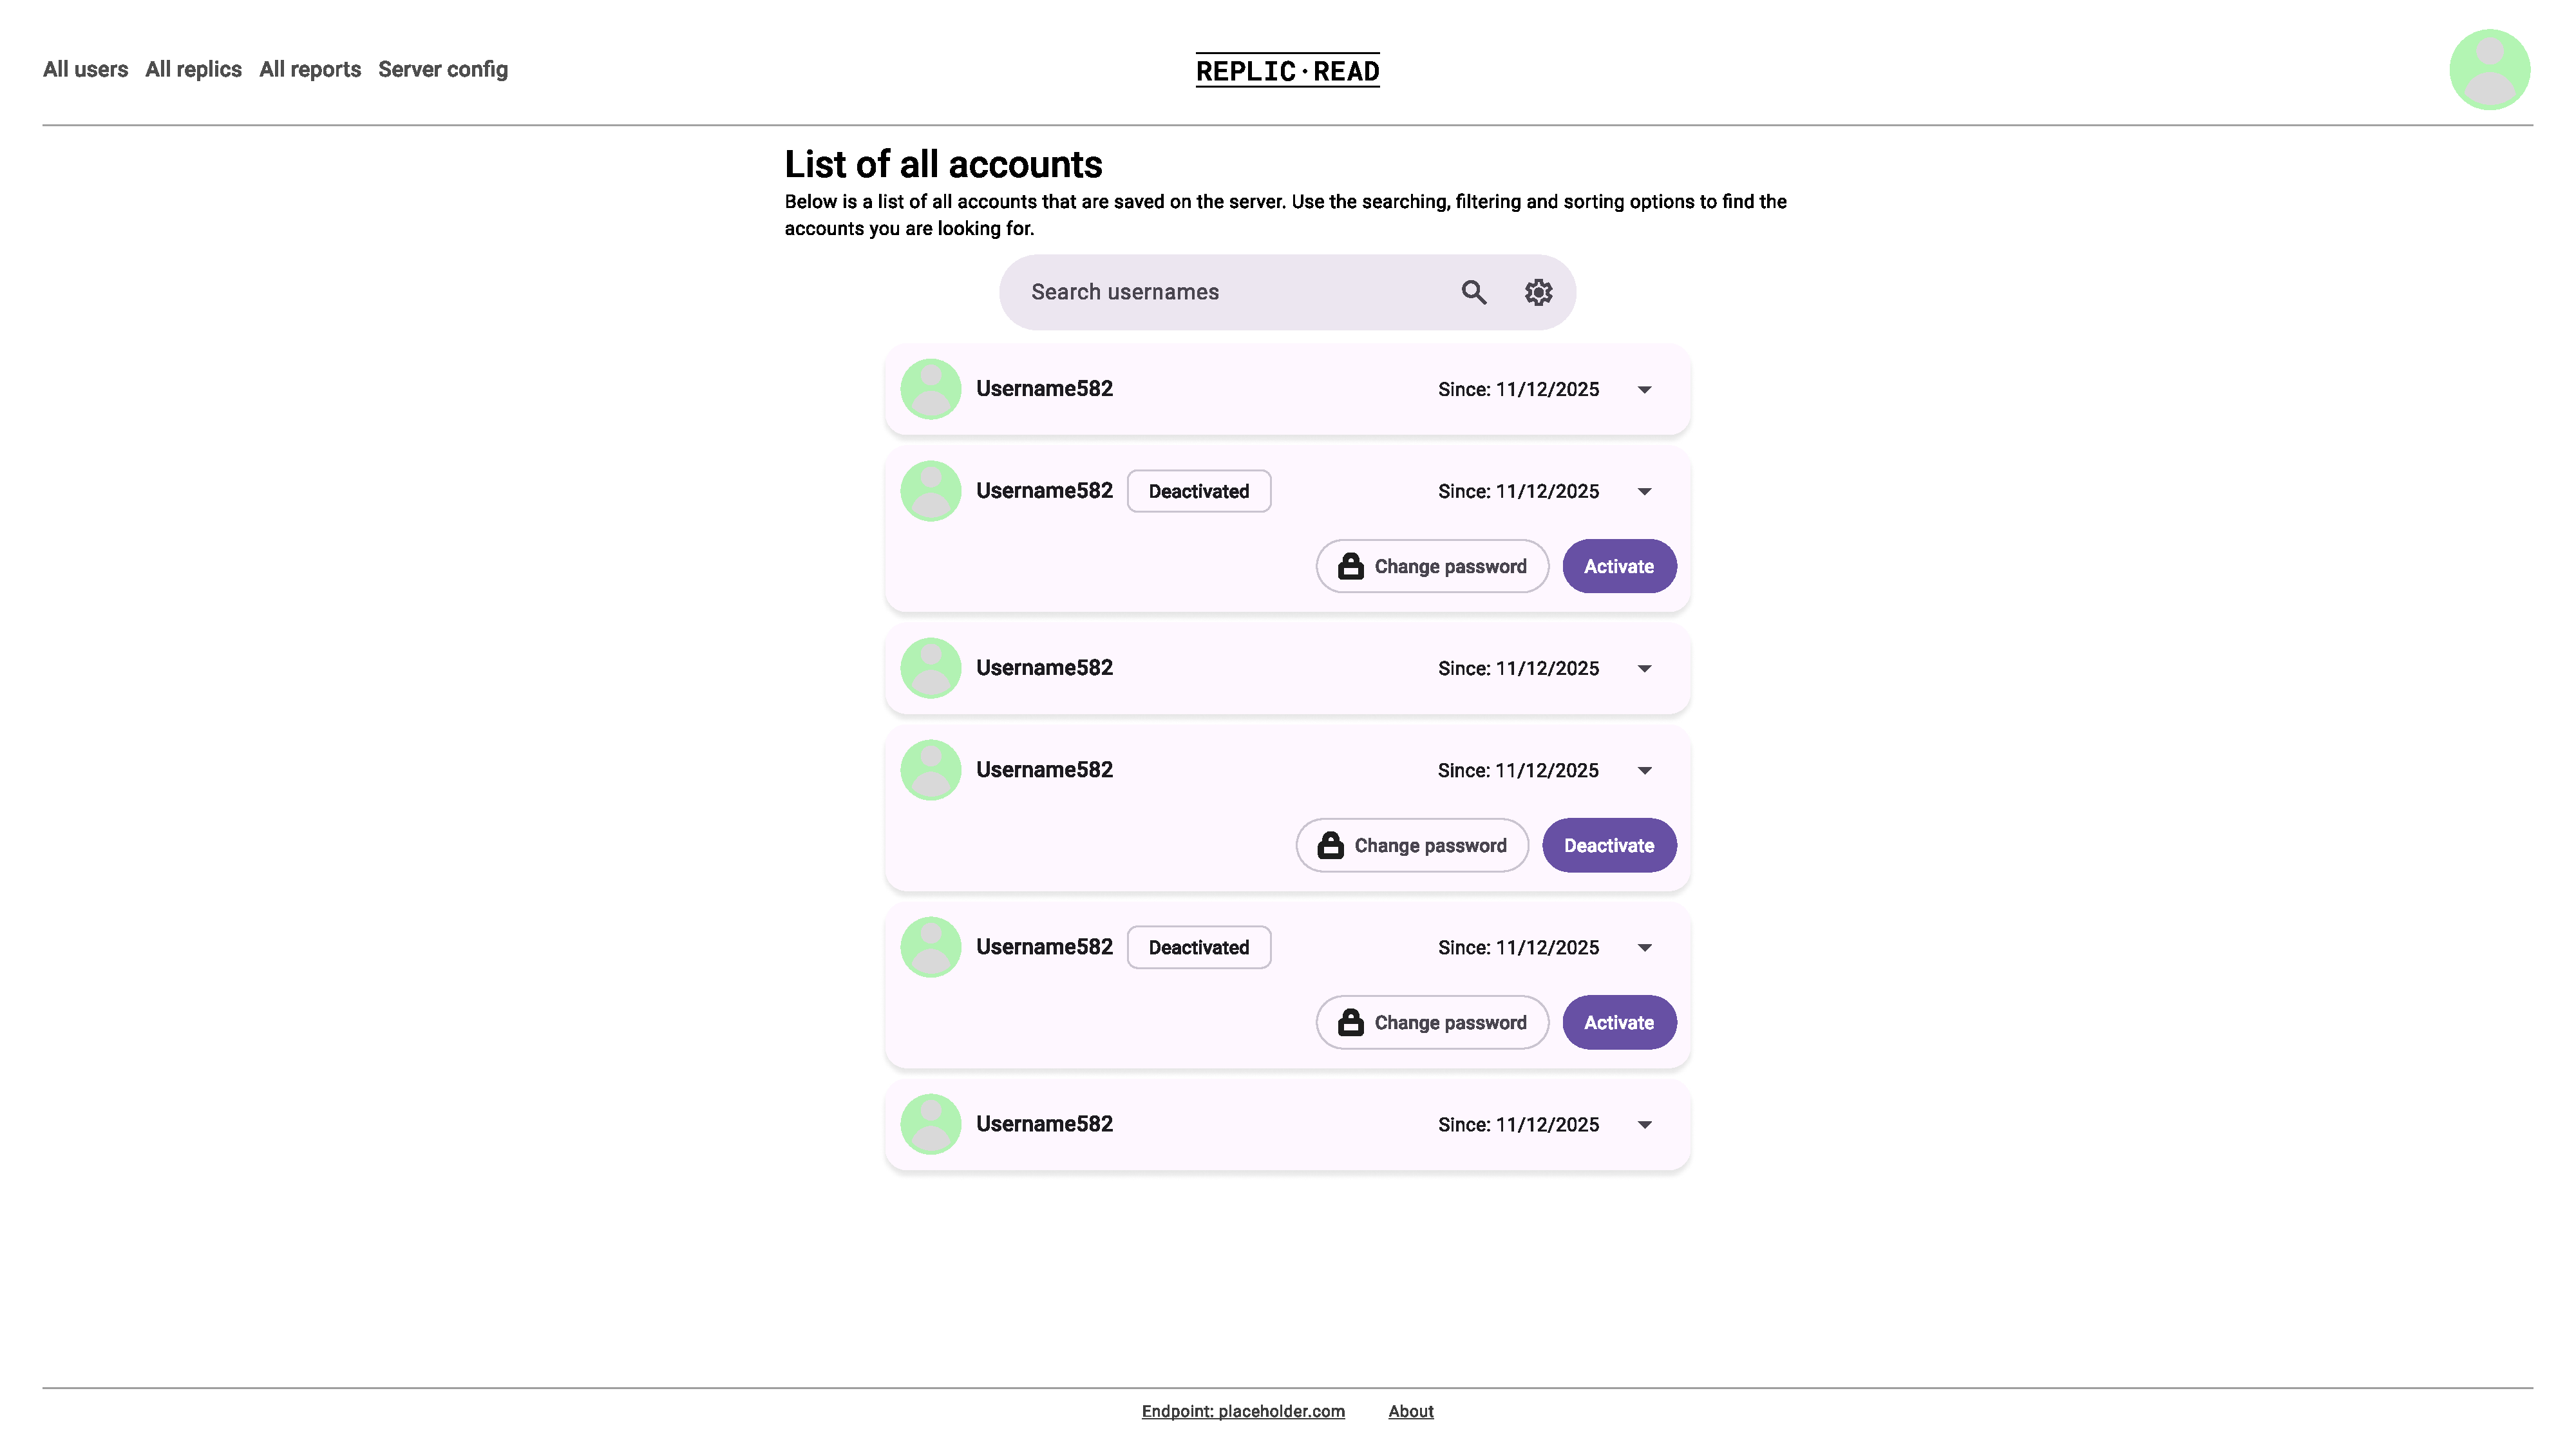
\includegraphics[width=12cm]{web-accounts-noconfig}}

    \caption{Admin accounts view}
    \label{fig:web-accounts-noconfig-view}
\end{figure}

\subsubsection{Admin reports view}
The admin reports view allows the admin to view all open reports that have been made (by users).
Each report is represented by an item in a list that shows the author, submission date and description.
Each item has context actions that allow the admin to review (\ref{subsubsec:review-report}) or close a report.
The reports can be searched using a search bar, and filtered/sorted by using the sorting config that can be expanded (\ref{fig:web-reports-config-view}) or collapsed (\ref{fig:web-reports-noconfig-view}).
\begin{figure}
    \centering
    \fbox{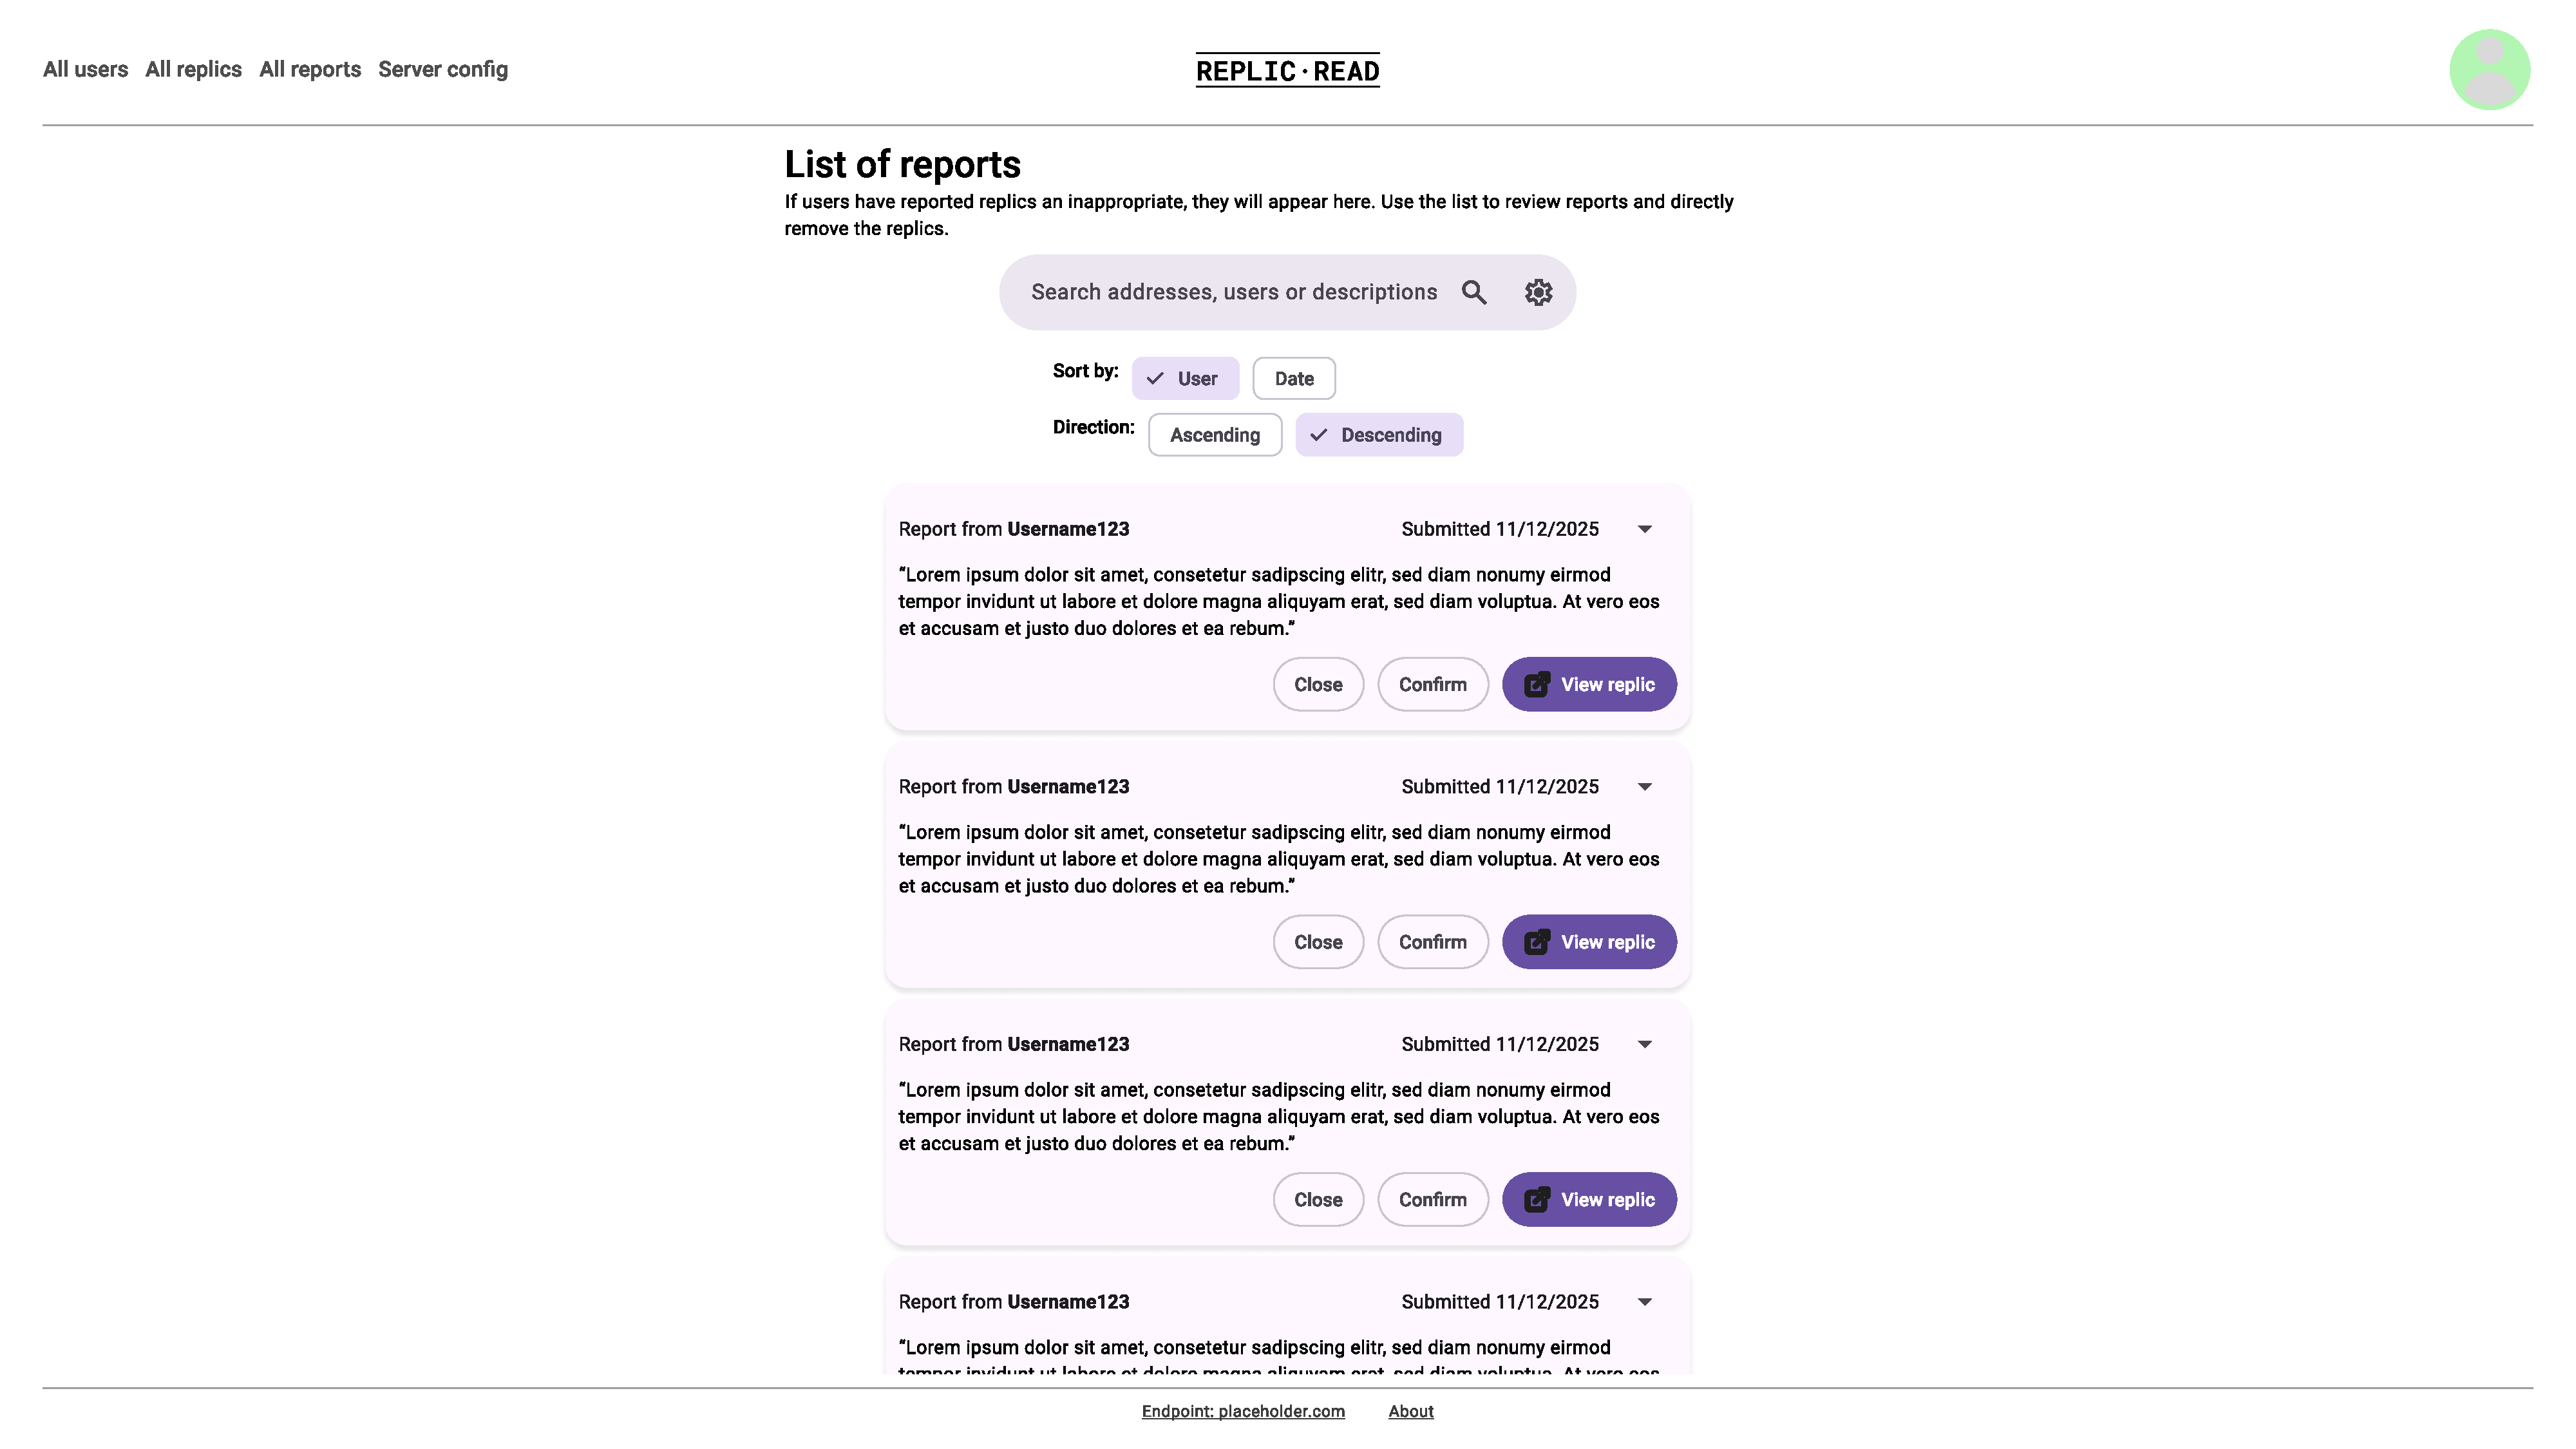
\includegraphics[width=12cm]{web-reports-config}}

    \caption{Admin reports view with search config visible}
    \label{fig:web-reports-config-view}
\end{figure}
\begin{figure}
    \centering
    \fbox{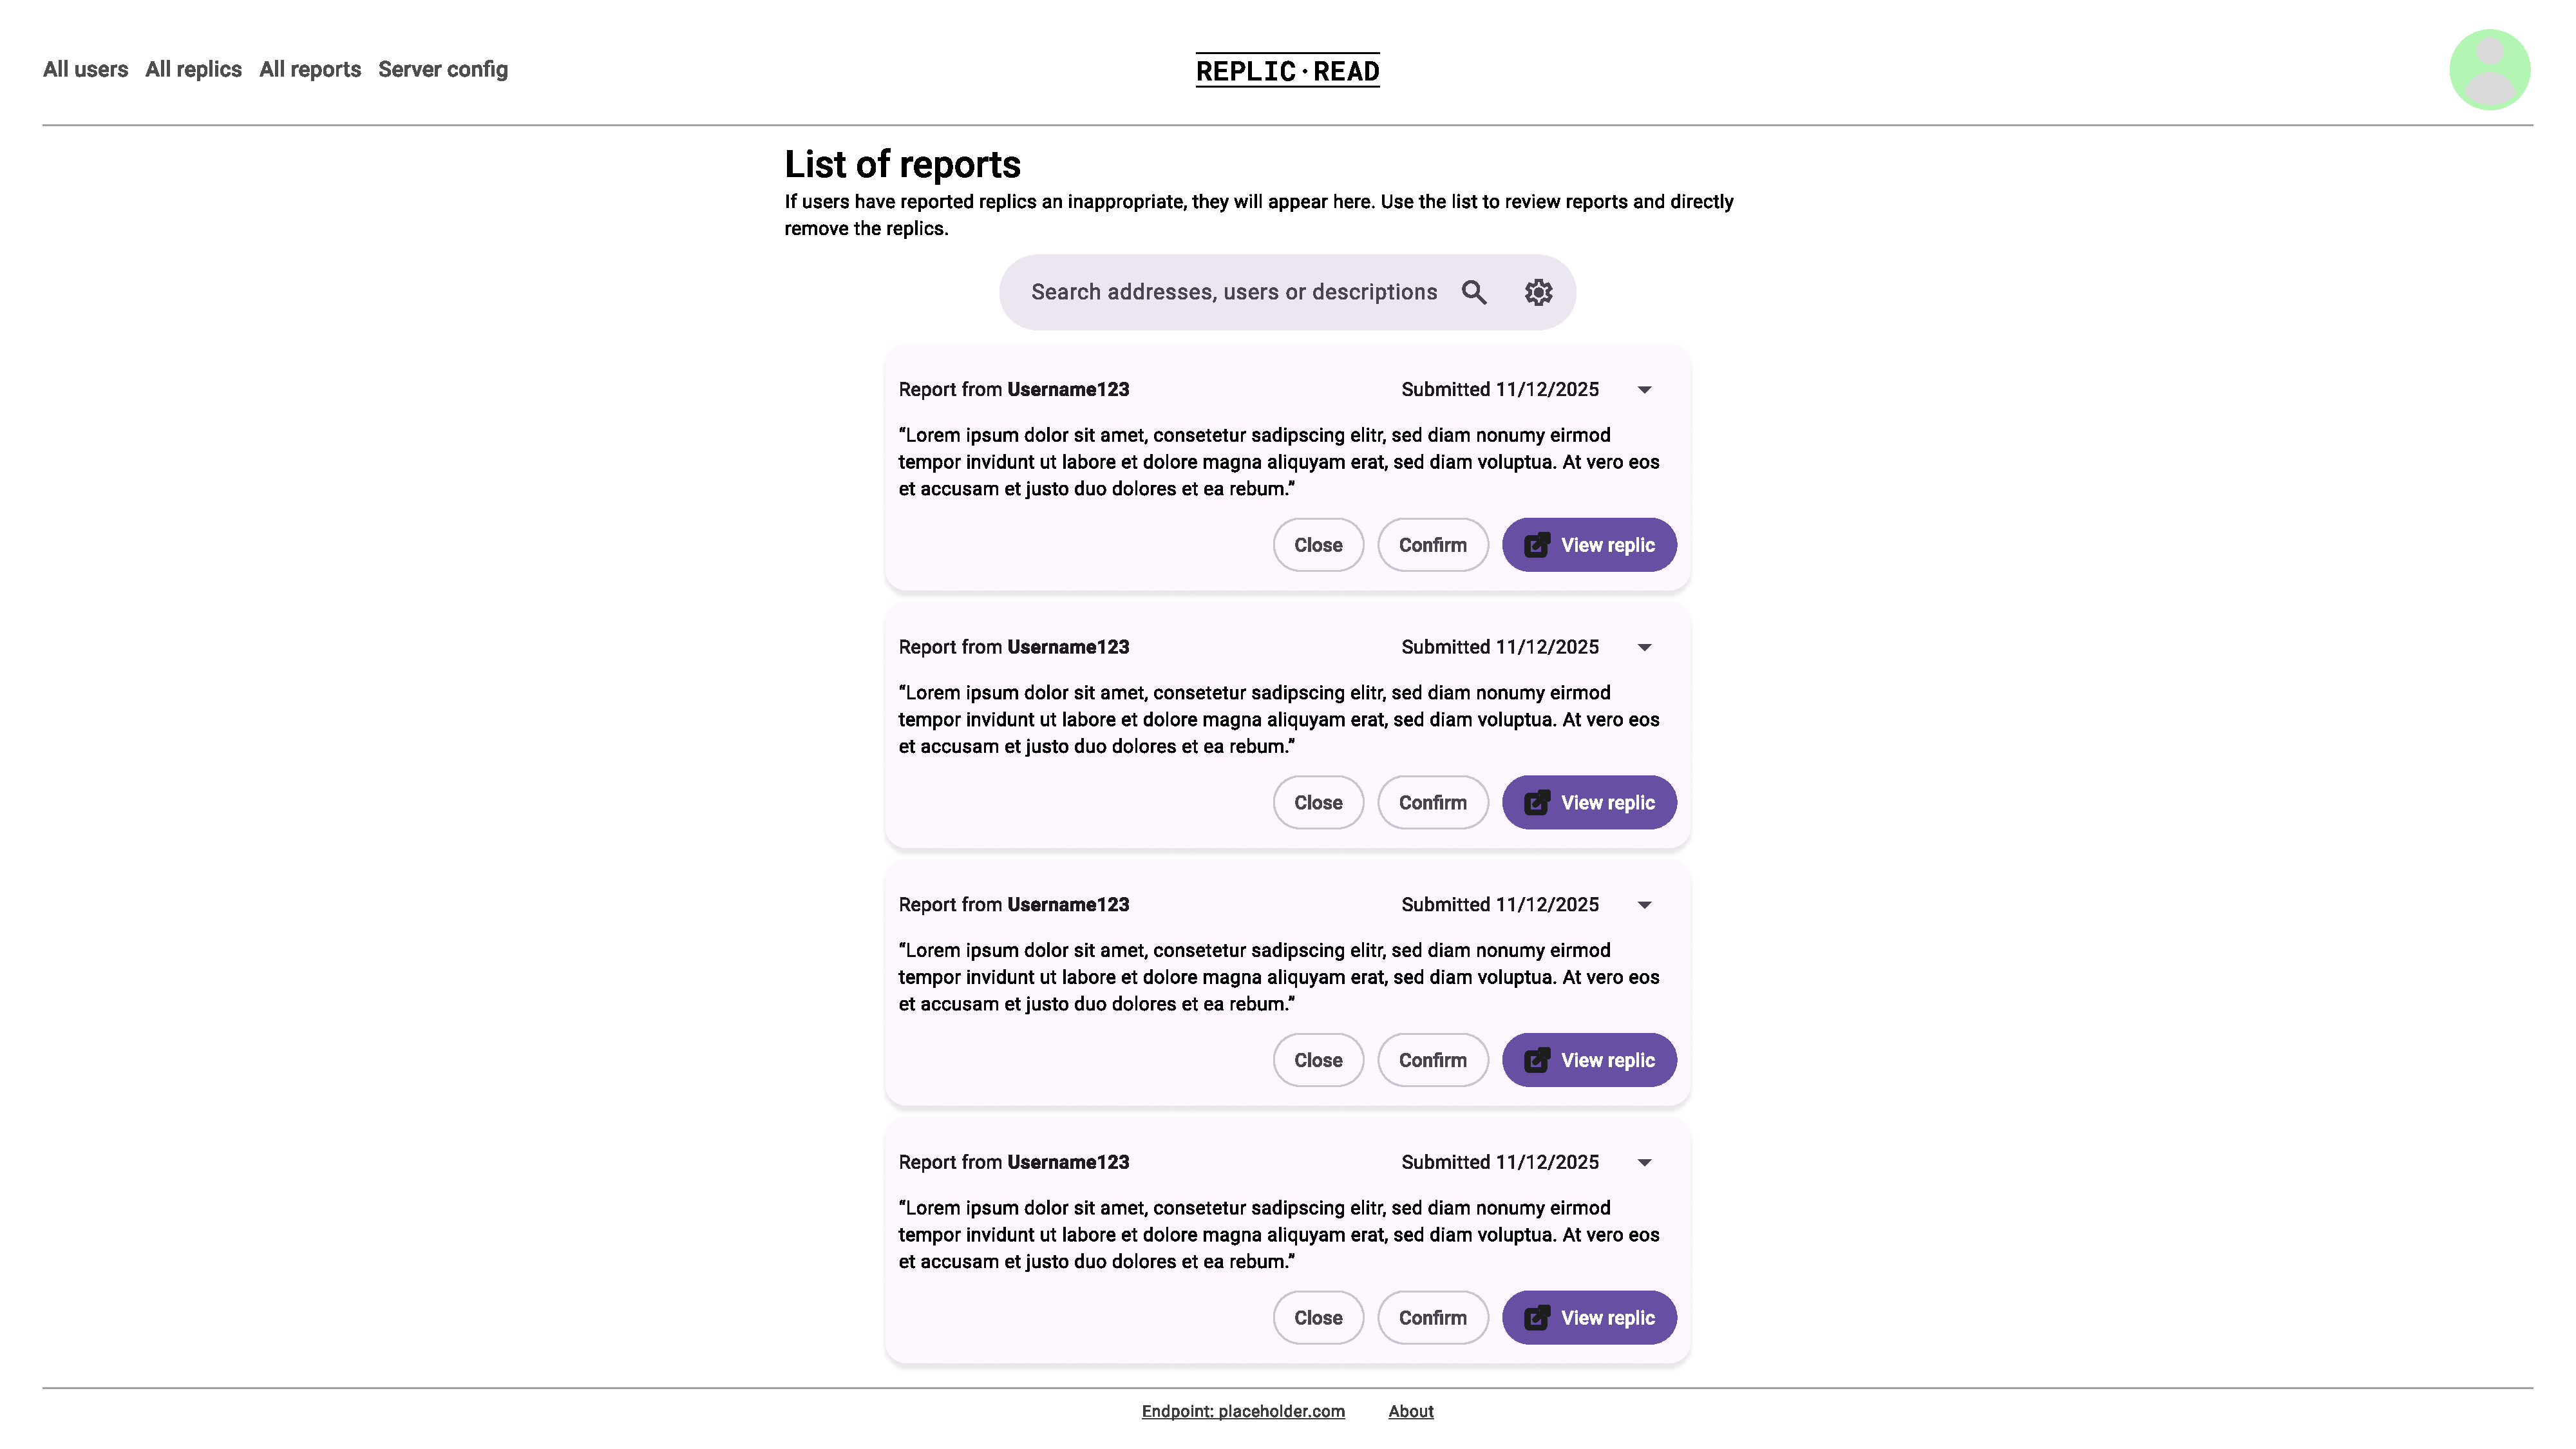
\includegraphics[width=12cm]{web-reports-noconfig}}

    \caption{Admin reports view}
    \label{fig:web-reports-noconfig-view}
\end{figure}

\subsubsection{Replic view}
The replic view (\ref{fig:web-replic-active-view}) shows information about a specific replic and allows the user to view the replic's content.
If the replic is not accessible anymore, it is shown to the user (\ref{fig:web-replic-inactive-view}).
\begin{figure}
    \centering
    \fbox{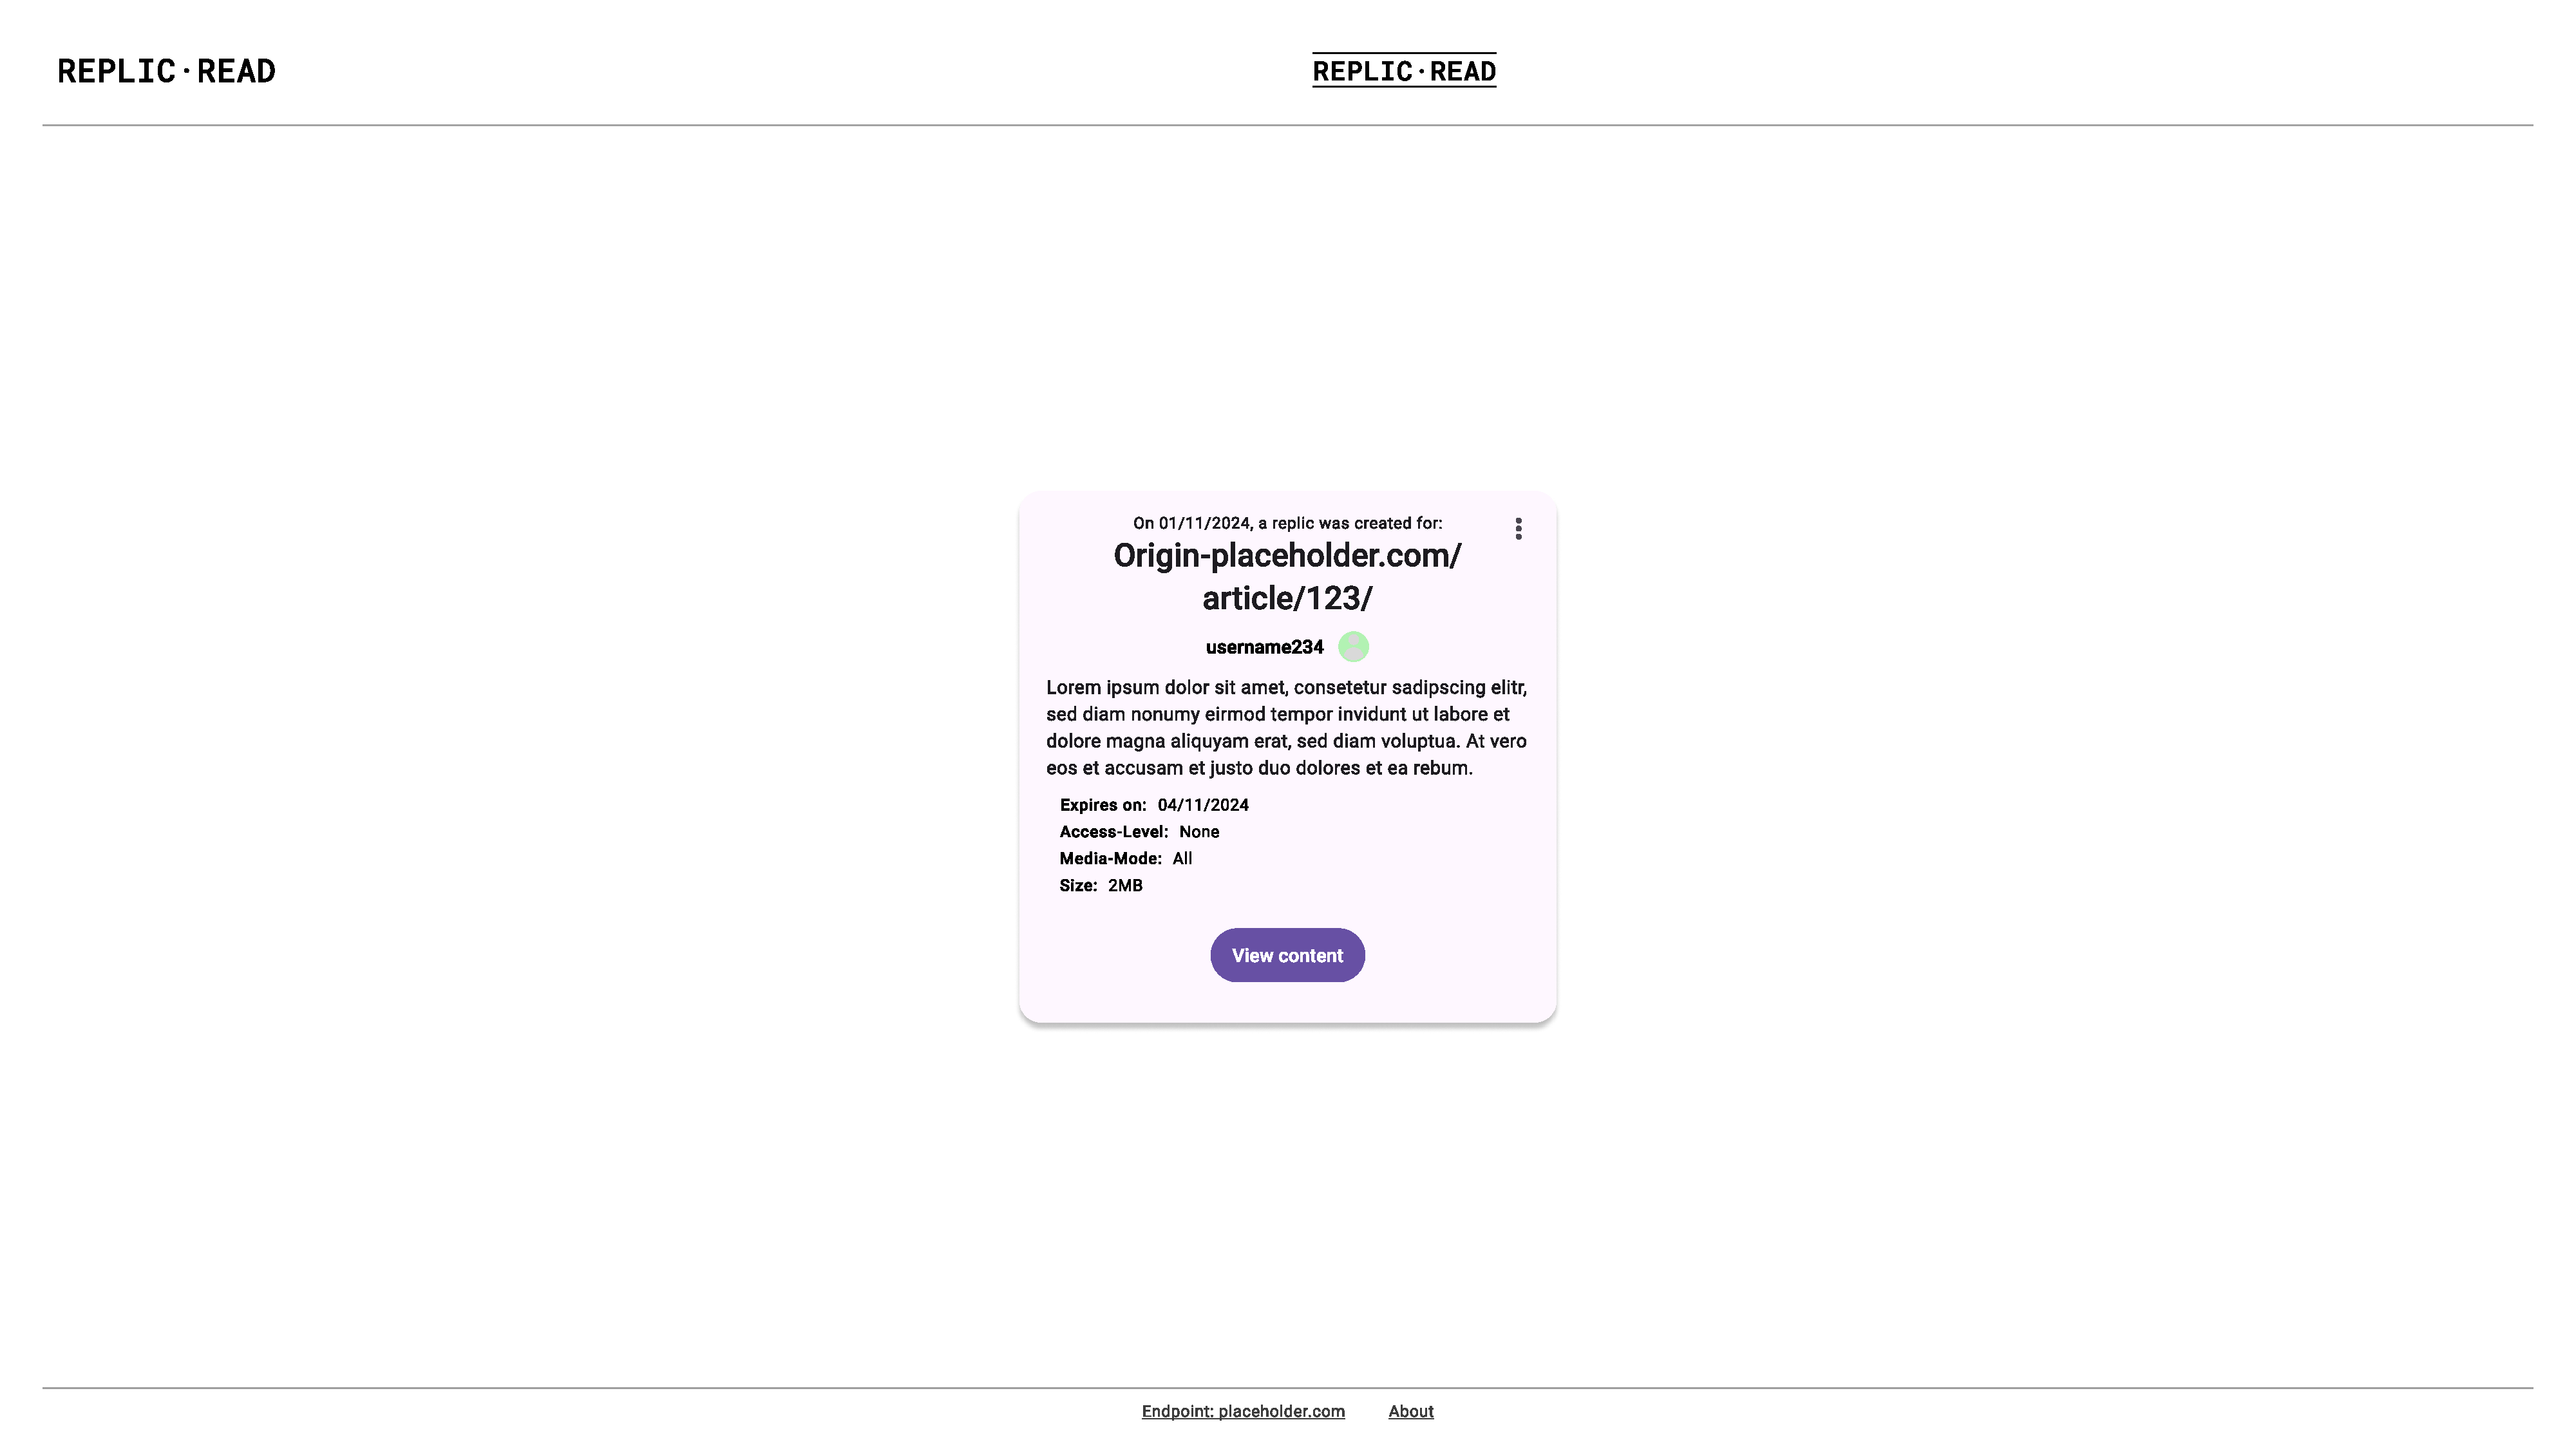
\includegraphics[width=12cm]{web-replic-active}}

    \caption{Active replic view}
    \label{fig:web-replic-active-view}
\end{figure}
\begin{figure}
    \centering
    \fbox{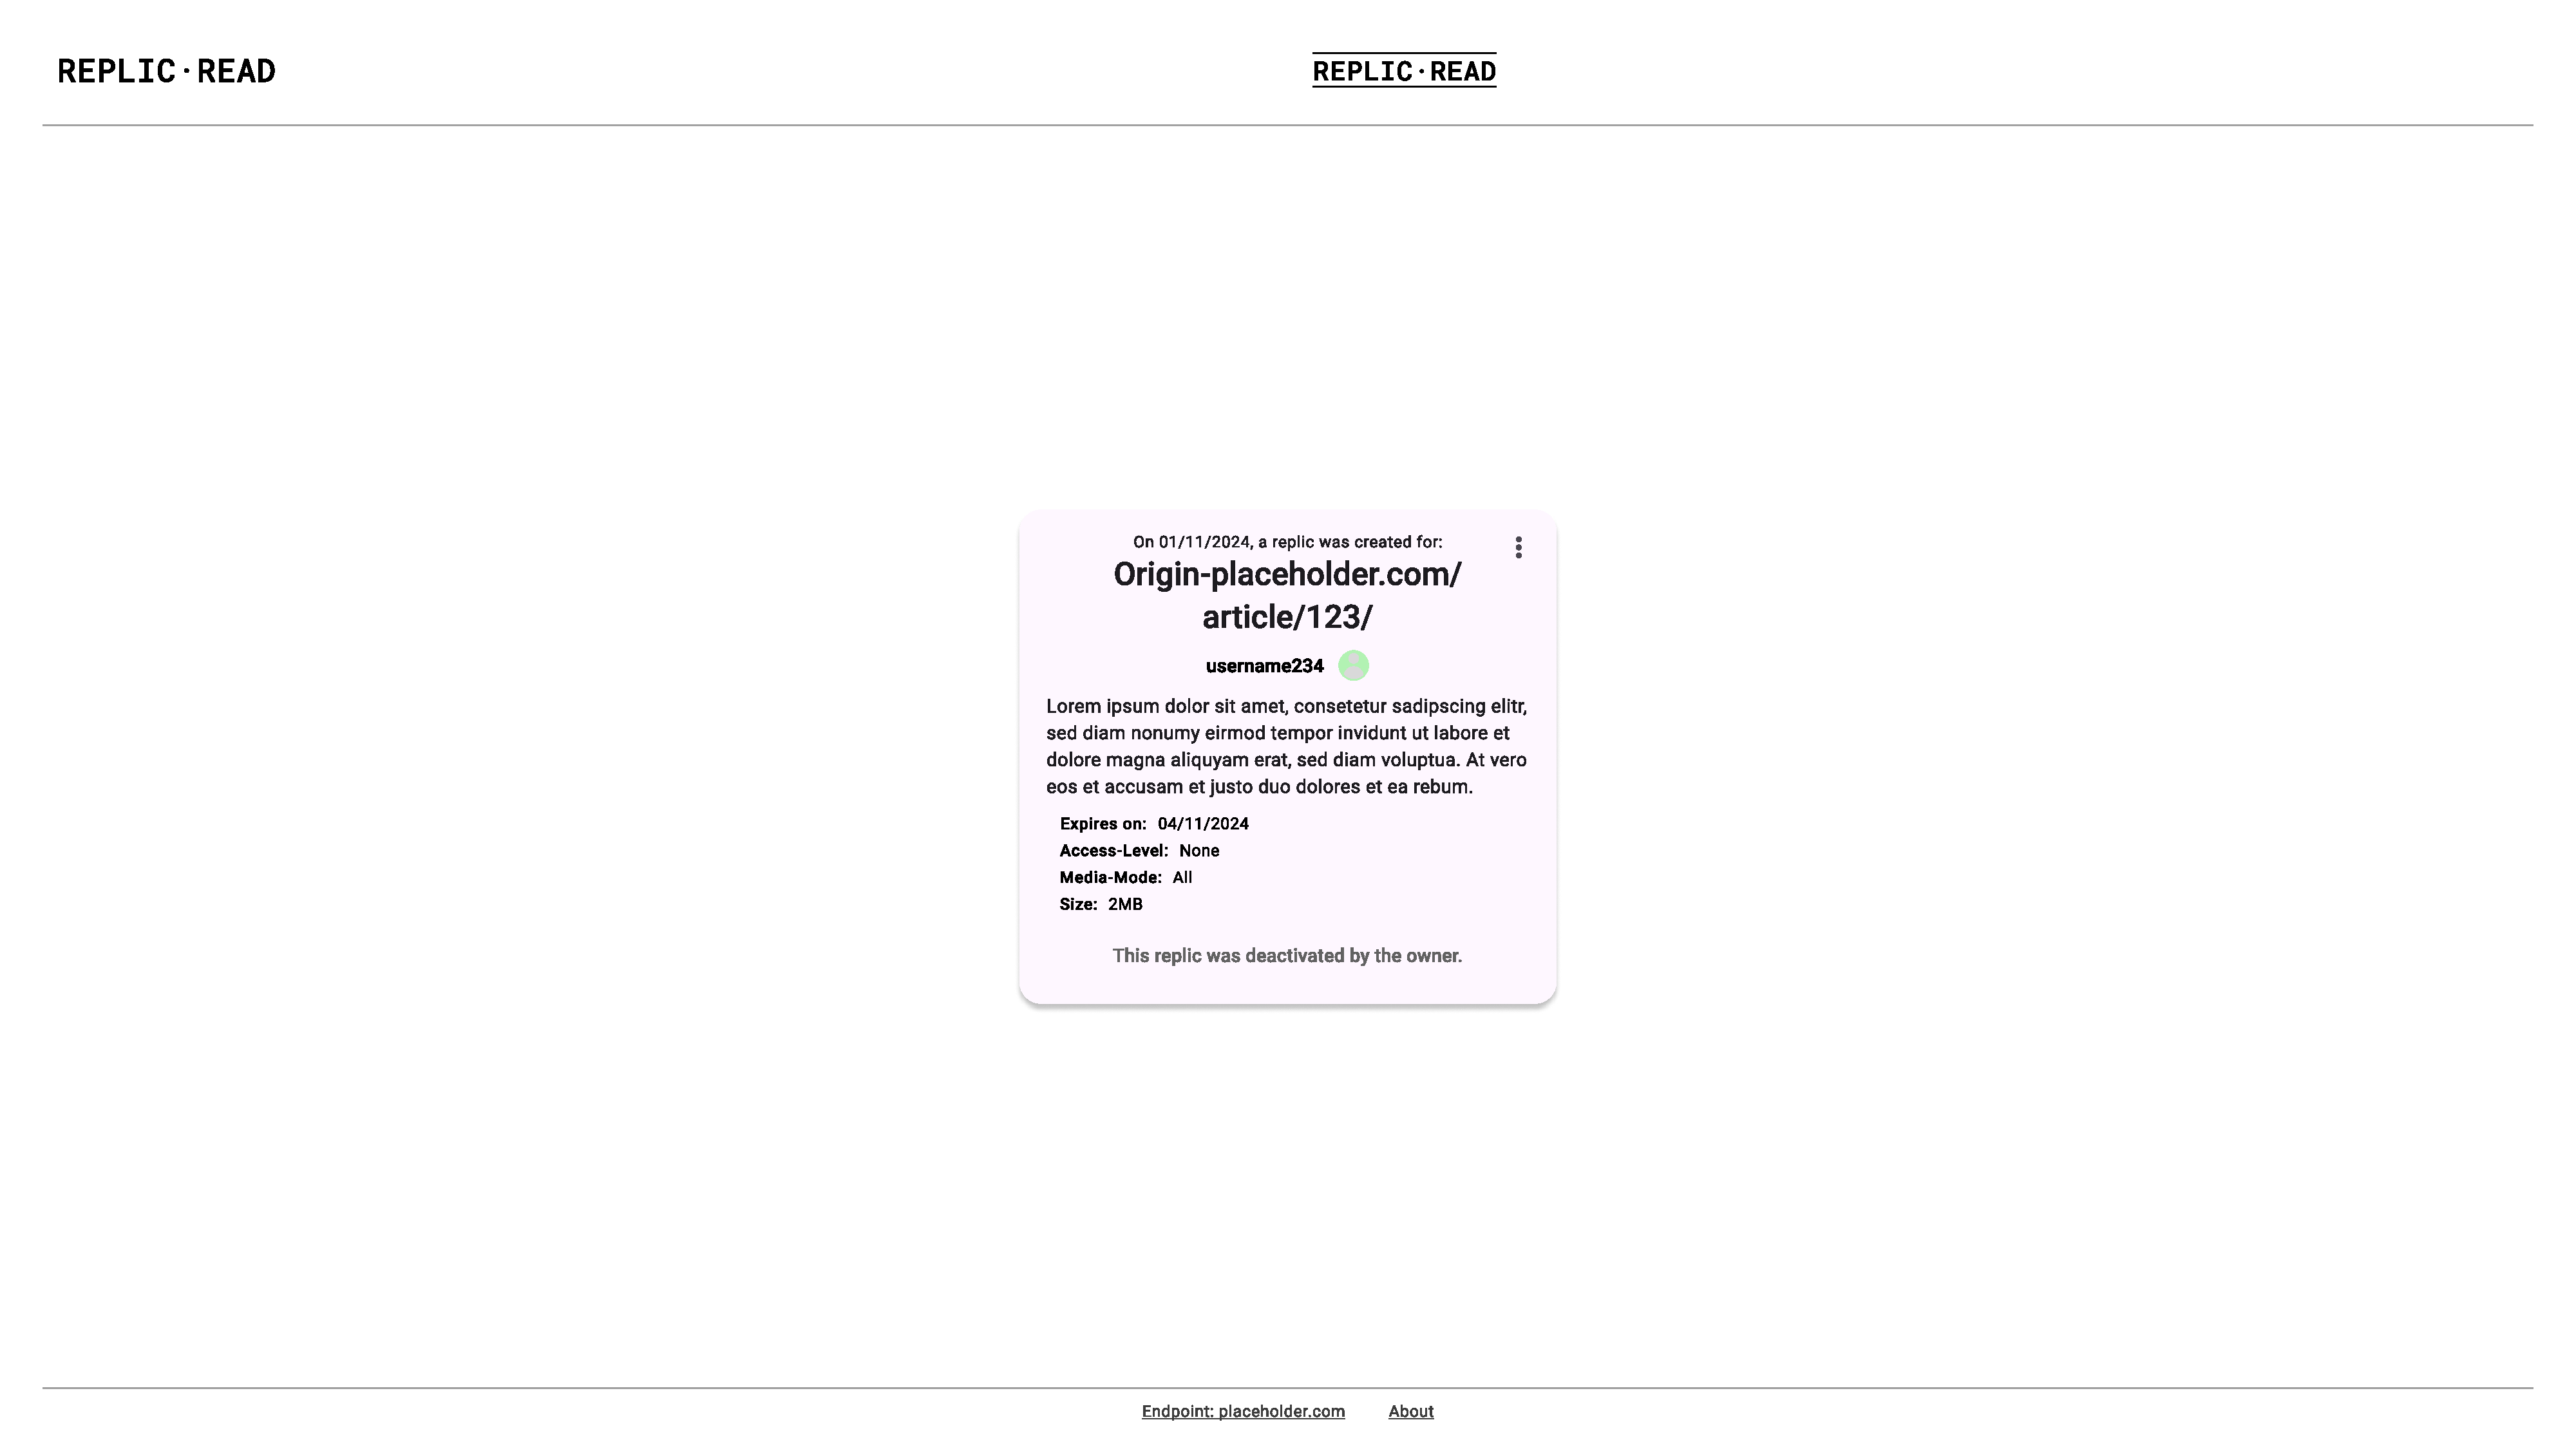
\includegraphics[width=12cm]{web-replic-inactive}}

    \caption{Inactive replic view}
    \label{fig:web-replic-inactive-view}
\end{figure}


    \section{Usage Scenarios}\label{sec:usage-scenarios}
    In this chapter, concrete usage examples are given to highlight the practical nature of the system.
Simon, Niklas, Jona and Meike will be normal users of the system, whereas Timo will be the server administrator with access to the admin-account.

\subsection{Login}\label{subsec:us-login}
Simon and Niklas are avid readers of a german newspaper.
To share their articles with the rest of the family, they create accounts (\ref{subsubsec:signup}): Simon uses the web-interface, Niklas creates the account from inside the browser-extension.

\subsection{Creating, sharing and accessing a replic}\label{subsec:us-creating-and-sharing-a-replic}
Simon reads an article that, he believes, his Brother Jona will also find interesting.
While the tab for the article is opened on his browser, he uses the extension, in which he is logged-in, to create a replic (\ref{subsubsec:create-replic}).
He sets an expiration date for one week.
After the replic is created, he copies the link to it (\ref{subsubsec:copy-replic-links}) and texts it to Jona. \newline
Jona receives the link via the messenger from Simon and clicks it.
His browser opens (\ref{subsubsec:select-replic}) and shows the replic overview (\ref{subsubsec:view-replic}), where he reads the description of the replic that Simon entered.
He proceeds to open the link and read the article.

\subsection{Accesing own replics}\label{subsec:us-accesing-own-replics}
After Jona liked the article so much, Simon is inclined to also share the article with Niklas.
So he doesn't have to create a new replic, he visits the replics view, goes to the replic screen for the only replic he owns, copies the link (\ref{subsubsec:copy-replic-links}) and sends it to Niklas.

\subsection{Accessing replic too late}\label{subsec:us-accessing-replic-too-late}
Because Niklas is busy, he only receives the link after a few days.
When he tries to access the replic, he cannot view it, due to the expiration date being met.

\subsection{Reporting a replic}\label{subsec:us-reporting-a-replic}
An anonymous user has created a replic and sent the link to Jona via E-mail.
After observing the replic (\ref{subsubsec:view-replic}), Jona realizes that the content is not appropriate.
He creates a report for the replic (\ref{subsubsec:report-replic}).

\subsection{Reviewing a report}\label{subsec:us-reviewing-a-report}
During hsi weekly admin-tour, Timo spots the report filed by Jona.
After checking the replic, he comes to the conclusion that the replic is not appropriate, reviews the report (\ref{subsubsec:review-report}) and removes the replic (\ref{subsubsec:remove-replic}).

\subsection{Creating and deactivating an account (Admin)}\label{subsec:us-creating-an-account-admin}
To encourage Meike to join the system, Timo creates an account for her on the admin-panel (\ref{subsubsec:create-user}) and shares the credentials with her.
However, Meike prefers to read newspapers in paper, which causes Timo to deactivate her account (\ref{subsubsec:deactivate-acc-admin}).

\subsection{Resetting password}\label{subsec:resetting-password}
Sadly, Simon is very occupied with other aspects of his life and doesn't use replic-read often.
He forgets his password.
To help him, Timo resets his password (\ref{subsubsec:reset-pass}) to allow him to login (\ref{subsubsec:login}) again.

\subsection{Changing account data}\label{subsec:changing-account-data}
After some time of not using the system, Simon is embarassed by the username, email and color he set up when he was just a small child.
To fix this, he changes his username (\ref{subsubsec:change-username}) and profile color (\ref{subsubsec:change-color}).
Additionally, he requests to change his email to his new, less embarassing, one (\ref{subsubsec:change-email}) and verifies it by clicking the link in the email that was sent to him.


    \section{Product environment}\label{sec:product-environment}
    \subsection{System achitecture}\label{subsec:system-achitecture}
The System contains of three main components:
\begin{itemize}
    \item The web-client
    \item The browser-extension
    \item The server
\end{itemize}.

Together, the web-client and browser-extension act as the client in the server-client architecture and depend on the server.

The web client will be implemented as a single-page web-app written in angular.js, while the browser extension will be implemented in react.
The server will be based on Java-Spring.

\subsection{Interfaces}\label{subsec:interfaces}
External interfaces the system accesses are
\begin{itemize}
    \item The user-interfaces described in~\ref{sec:user-interface}
    \item The browser-interface to access html content rendered to the user
\end{itemize}.

Internally, following interfaces are provided:
\begin{itemize}
    \item A REST-interface provided by the server and used by the clients
    \item An interface that provides the html-files of the replics, provided by the server
    \item An SQL-Database that is used by the server.
\end{itemize}

\end{document}